\documentclass{beamer}
%%%%%% UNOFFICIAL ICL BEAMER TEMPLATE V.0.1 %%%%%%
% This is a basic LaTeX Beamer template that I customised to have the logo of ICL and a background picture. Mind that this is NOT an official ICL template but it may still be useful for informal presentations.
% The official ICL graphical identity resources can be found here: http://www3.imperial.ac.uk/graphicidentity
% Please drop me an e-mail or comment via Twitter @AJunyentFerre if you found this was useful or have any suggestion to improve it.
%%%%%%

\usepackage[english]{babel}
\usepackage{xcolor}
\usepackage{xmpmulti}
\usepackage{amsmath}
\usepackage[mathscr]{eucal}
%\usepackage{eucal}
\usepackage{pgf}
\usepackage{pgfplots}
\usepackage{wrapfig}
\usepackage{tikz}
\usepackage{url}
\usepackage{graphicx}
\usepackage{subfig}
\usepackage{dsfont}
\usepackage{xcolor}
\usepackage{colortbl}
\usepackage{pgfplots}
\usepackage{highlight}
\usepackage{collcell}
\usepackage{tabularx}
\usepackage{textcomp}
\usepackage{xstring}
\usepackage{appendixnumberbeamer}

\usepgfplotslibrary{groupplots}
\usetikzlibrary{pgfplots.groupplots,arrows.meta,shadows,positioning,angles,quotes}
\usetikzlibrary{matrix,chains,positioning,decorations.pathreplacing,arrows}
\usepackage{tikz}
\usetikzlibrary{shapes.geometric}
\usetikzlibrary{positioning}

\usepgfplotslibrary{fillbetween}

\newcommand*\circled[1]{\tikz[baseline=(char.base)]{
            \node[shape=circle,draw,inner sep=0.5pt] (char) {#1};}}
\renewcommand{\vec}[1]{\mathbf{#1}
}
\newcommand{\colorpos}{green}
\newcommand{\colorneg}{red}

\newcommand{\fix}{\marginpar{FIX}}
\newcommand{\new}{\marginpar{NEW}}


\DeclareMathOperator*{\argmax}{arg\,max}
\def\checkmark{\tikz\fill[scale=0.4](0,.35) -- (.25,0) -- (1,.7) -- (.25,.15) -- cycle;} 
\definecolor{webgreen}{rgb}{0,.5,0}
\definecolor{webbrown}{rgb}{.6,0,0}
\definecolor{Maroon}{cmyk}{0, 0.87, 0.68, 0.32}
\definecolor{RoyalBlue}{cmyk}{1, 0.50, 0, 0}
\definecolor{Black}{cmyk}{0, 0, 0, 0}
\definecolor{skymagenta}{rgb}{0.81, 0.44, 0.69}

%%%%%% THE FOLLOWING FILE CONTAINS THE STYLE DEFINITIONS %%%%%%
\usepackage[utf8]{inputenc}
\usepackage[export]{adjustbox}

\definecolor{gris}{rgb}{0.92,0.92,0.92}
\definecolor{blau-upc}{rgb}{.192,.365,.506}

\setbeamercolor{titlelike}{fg=blau-upc}
% \setbeamercolor{barra}{bg=white,fg=white}
\setbeamercolor{capcalera}{bg=blau-upc,fg=white}
\setbeamercolor{section in toc}{fg=blau-upc}
\setbeamertemplate{sections/subsections in toc}[circle]
\setbeamertemplate{itemize items}[circle]
\setbeamercolor{item}{fg=blau-upc}
\setbeamertemplate{blocks}[rounded][shadow=true]
\setbeamercolor*{block body}{bg=gris}
\setbeamerfont{block body}{size=\footnotesize}
\setbeamercolor*{block title}{parent=structure,bg=blau-upc,fg=white}

\setbeamersize{text margin left=12mm,text margin right=12mm}
\setbeamertemplate{navigation symbols}{}

\setbeamertemplate{footline}[frame number]{}


\defbeamertemplate*{headline}{infolines theme}
{
	\begin{beamercolorbox}[wd=\paperwidth,ht=6.5mm,right]{white}%
		%
\includegraphics[width = 45mm, height=10mm]{./logotips/visapp}\hspace*{2mm}\vskip0.2ex
	\end{beamercolorbox}
 	\begin{beamercolorbox}[wd=\paperwidth,ht=0.5mm,left]{barra}%
 		\hspace*{1mm}
 	\end{beamercolorbox}
}

\setbeamertemplate{footline}
{
	\hbox{
	\begin{beamercolorbox}[wd=0.1\paperwidth,ht=10mm,left]{}
% 		\hspace*{1ex}
\includegraphics[height=8mm]{./logotips/imperiallogo.pdf}\vskip 2ex
	\end{beamercolorbox}
	\begin{beamercolorbox}[wd=0.8\paperwidth,ht=3ex,center]{}
		\hspace*{4ex}\insertsection\vskip 4ex
	\end{beamercolorbox}
	\begin{beamercolorbox}[wd=0.1\paperwidth,ht=3ex,right]{}
		\insertpagenumber\hspace*{6ex}\vskip 4ex
	\end{beamercolorbox}
	}
}

\setbeamertemplate{title page}
{
	\vbox{}
	\vfill
	\begin{centering}
		{\usebeamerfont{title}\usebeamercolor[fg]{title}\inserttitle}
		\vskip0.2em
		{\usebeamerfont{subtitle}\usebeamercolor[fg]{subtitle}\insertsubtitle}
		\vskip2em\par
		\small\insertauthor\par
		\vskip2em\par
		\tiny\insertdate\vskip1em\par
	\end{centering}
% 	\vfill
}

%\usebackgroundtemplate{\put(-50,-340){\includegraphics[width=10cm]{}}} 

%%%%%%

%%%%%% TITLE, AUTHOR, DATE DEFINITIONS %%%%%%
\title{Contributions to Deep Transfer Learning}
\subtitle{From Supervised to Reinforcement Learning}
\author{\textbf{Matthia Sabatelli} \\ Montefiore Institute, Department of Electrical Engineering and Computer Science, Universit\'e de Li\`ege, Belgium}


\date{March 30th 2022}
%%%%%%

\setbeamertemplate{footline}[frame number]{}


\begin{document}

\frame{\titlepage} 

\frame{\frametitle{Presentation outline}\tableofcontents}

%============================================================================

\begin{frame}
	\section{Part I: Preliminaries}
	\subsection{Transfer Learning}

	\begin{center}
		\textcolor{skymagenta}{\textbf{PART I}}
	\end{center}
\end{frame}

\begin{frame}{Transfer Learning}
	\begin{figure}
		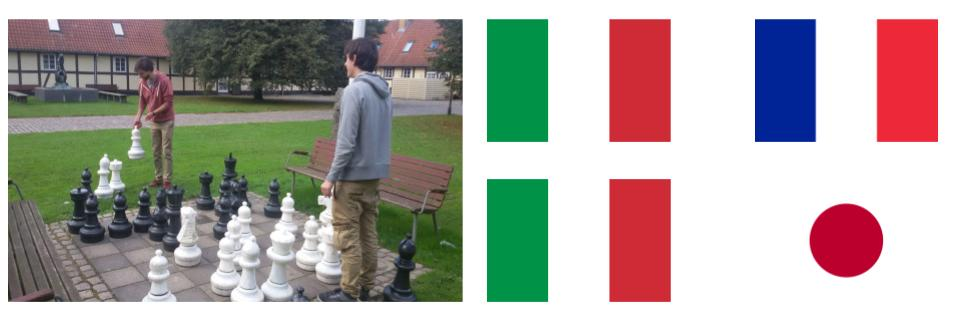
\includegraphics[width=1\textwidth]{figures/example}
	\end{figure}

\end{frame}


\iffalse
\begin{frame}{Transfer Learning}
	


	\begin{columns}
		\begin{column}{.5\textwidth}
			On the one hand we have the concept of \textcolor{RoyalBlue}{\textbf{source}} $S$, which is needed to build some prior knowledge available for transfer
		
		\bigskip
		\begin{itemize}
			\item	Source Domain $\mathcal{D}_S$
			\item	Source Task $\mathcal{T}_S$
		\end{itemize}

		\end{column}
		
		\begin{column}{.5\textwidth}
			While on the other hand we have the concept of \textcolor{RoyalBlue}{\textbf{target}} $T$, defining the machine learning problem we would like to solve
		
		\bigskip
		\begin{itemize}
			\item Target Domain $\mathcal{D}_T$
			\item Target Task $\mathcal{T}_T$
		\end{itemize}


		\end{column}
		
	\end{columns}



\end{frame}
\fi


\begin{frame}{Transfer Learning}
	
	\bigskip
	Transfer Learning in practice ...
	\bigskip
	\begin{figure}[ht!]
  \begin{tikzpicture}[scale = 0.35]
      \begin{axis}[
	name=ax1,
      	grid style={dashed,gray},
      	grid = both, 
      	tick style=black,
	title=Learning Speed Improvements,
        xlabel=Training Iterations,
        ylabel=Performance,
      ]


      %\addlegendentry{Pre-trained Model} 
      \addlegendentry{Scratch Model}  
      
      %\addplot [ultra thick, blue, mark=.] table [y=Transfer, x=episodes]
      %{./Chapter03/logs/speed_improvements.txt};
       \addplot [ultra thick, orange, mark=.] table [y=No-Transfer, x=episodes]
      {./Chapter03/logs/speed_improvements.txt};
     
      \legend{}

      \end{axis}

      \begin{axis}[
      	at={(ax1.south east)},
	xshift=2cm,
	grid style={dashed,gray},
      	grid = both, 
      	tick style=black,
	title=Jumpstart Improvements,
        xlabel=Training Iterations,
        ylabel=Performance,
      ]



      %\addlegendentry{Pre-trained Model} 
      \addlegendentry{Scratch Model}  
      
      %\addplot [ultra thick, blue, mark=.] table [y=Transfer, x=episodes]
      %{./Chapter03/logs/jumpstart_improvements.txt};
       \addplot [ultra thick, orange, mark=.] table [y=No-Transfer, x=episodes]
      {./Chapter03/logs/jumpstart_improvements.txt};
     
      \legend{}

      \end{axis}


      \begin{axis}[
	at={(ax1.south east)},
	xshift=-2cm,
      	yshift=-8cm,
	grid style={dashed,gray},
      	grid = both, 
      	tick style=black,
	title=Asymptotic Improvements,
        xlabel=Training Iterations,
        ylabel= Performance,
	legend columns=4, 
        legend style={font=\Large, at={(0.25,-0.3,-0.4)},anchor=north west,legend columns=3},
      ]


      %\addlegendentry{Pre-trained Model} 
      \addlegendentry{Scratch Model}  
 
      %\addplot [ultra thick, blue, mark=.] table [y=Transfer, x=episodes]
      %{./Chapter03/logs/asymptotic_improvements.txt};
      \addplot [ultra thick, orange, mark=.] table [y=No-Transfer, x=episodes]
      {./Chapter03/logs/asymptotic_improvements.txt};
       
      \end{axis}
	\end{tikzpicture}
\end{figure}



\end{frame}


\begin{frame}{Transfer Learning}
	
	\bigskip
	Transfer Learning in practice ...
	\bigskip
	\begin{figure}[ht!]
  \begin{tikzpicture}[scale = 0.35]
      \begin{axis}[
	name=ax1,
      	grid style={dashed,gray},
      	grid = both, 
      	tick style=black,
	title=Learning Speed Improvements,
        xlabel=Training Iterations,
        ylabel=Performance,
      ]


      \addlegendentry{Pre-trained Model} 
      \addlegendentry{Scratch Model}  
      
      \addplot [ultra thick, blue, mark=.] table [y=Transfer, x=episodes]
      {./Chapter03/logs/speed_improvements.txt};
       \addplot [ultra thick, orange, mark=.] table [y=No-Transfer, x=episodes]
      {./Chapter03/logs/speed_improvements.txt};
     
      \legend{}

      \end{axis}

      \begin{axis}[
      	at={(ax1.south east)},
	xshift=2cm,
	grid style={dashed,gray},
      	grid = both, 
      	tick style=black,
	title=Jumpstart Improvements,
        xlabel=Training Iterations,
        ylabel=Performance,
      ]



      \addlegendentry{Pre-trained Model} 
      \addlegendentry{Scratch Model}  
      
      \addplot [ultra thick, blue, mark=.] table [y=Transfer, x=episodes]
      {./Chapter03/logs/jumpstart_improvements.txt};
       \addplot [ultra thick, orange, mark=.] table [y=No-Transfer, x=episodes]
      {./Chapter03/logs/jumpstart_improvements.txt};
     
      \legend{}

      \end{axis}


      \begin{axis}[
	at={(ax1.south east)},
	xshift=-2cm,
      	yshift=-8cm,
	grid style={dashed,gray},
      	grid = both, 
      	tick style=black,
	title=Asymptotic Improvements,
        xlabel=Training Iterations,
        ylabel= Performance,
	legend columns=4, 
        legend style={font=\Large, at={(-0.1,-0.3,-0.4)},anchor=north west,legend columns=3},
      ]


      \addlegendentry{Pre-trained Model} 
      \addlegendentry{Scratch Model}  
 
      \addplot [ultra thick, blue, mark=.] table [y=Transfer, x=episodes]
      {./Chapter03/logs/asymptotic_improvements.txt};
      \addplot [ultra thick, orange, mark=.] table [y=No-Transfer, x=episodes]
      {./Chapter03/logs/asymptotic_improvements.txt};
       
      \end{axis}
	\end{tikzpicture}
\end{figure}



\end{frame}

\begin{frame}{Transfer Learning}

	The family of machine learning models that is studied under the lens of transfer learning is that of \textcolor{RoyalBlue}{Convolutional Neural Networks}
	\bigskip
	\begin{itemize}
		\item One of the main architectures when it comes to high-dimensional and spatially organized inputs
		\item Have achieved state-of-the-art results across many different machine learning problems
		\item We focus our analysis on Supervised Learning and Reinforcement Learning
	\end{itemize}


\end{frame}

\begin{frame}{Transfer Learning}
	
	When it comes to Supervised Learning ...
	\bigskip	
	\begin{figure}
		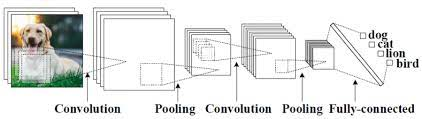
\includegraphics[width=1\textwidth]{figures/dogo}
	\end{figure}


\end{frame}

\begin{frame}{Transfer Learning}

	When it comes to Reinforcement Learning ...
	\bigskip

	\begin{figure}
		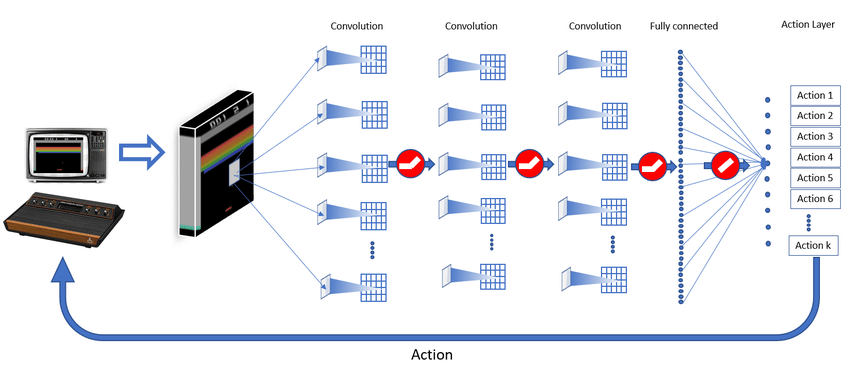
\includegraphics[width=1\textwidth]{figures/dqn}
		\caption{Image courtesy of Patel et al. (2019)}
	\end{figure}

\end{frame}



\begin{frame}{Transfer Learning}

	Why is Transfer Learning so interesting?

	\begin{itemize}
		\item It allows us to train deep learning models when there is a \textcolor{Maroon}{lack} of training data
		\item Is useful when computational resources are \textcolor{Maroon}{scarce}
		\item Results in \textcolor{RoyalBlue}{better performing} models
		\item Provides a unique tool for \textcolor{RoyalBlue}{better understanding} neural networks  
		\item Having models that generalize and transfer across different domains and tasks is \textcolor{RoyalBlue}{key} for the development of Artificial Intelligence 
	\end{itemize}


\end{frame}

%============================================================================

\begin{frame}
	\begin{center}
		\textcolor{skymagenta}{\textbf{PART II}}
	\end{center}
\end{frame}

\begin{frame}
	\begin{figure}
		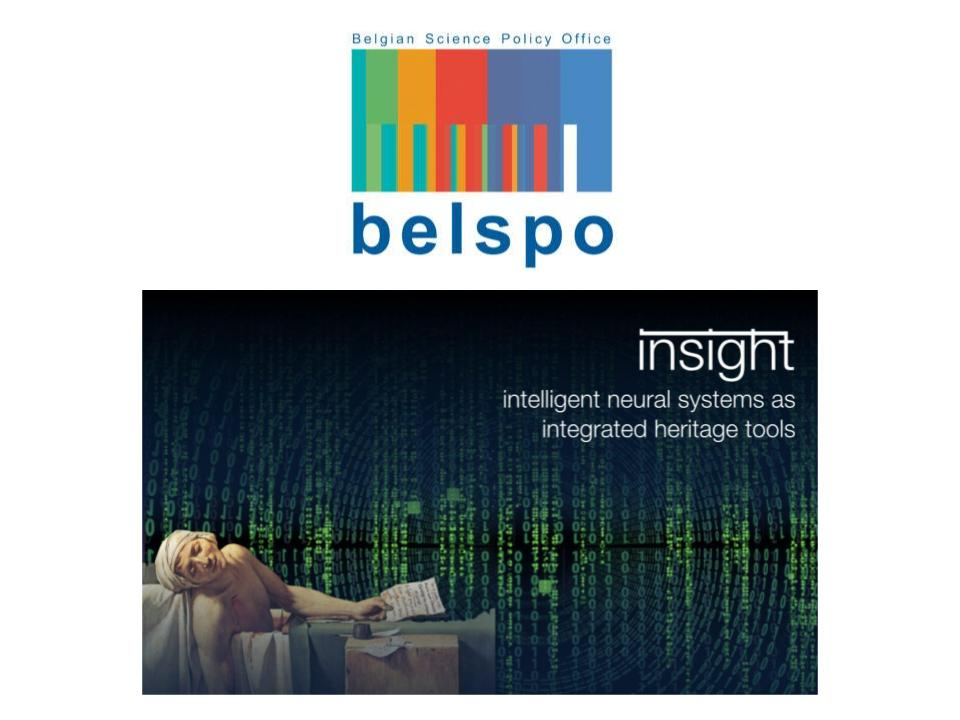
\includegraphics[width=1\textwidth]{figures/insight}
	\end{figure}
\end{frame}


\begin{frame}
	\section{Part II: Supervised Learning}
	\subsection{On the Transferability of Convolutional Neural Networks}

	We start by defining the components of \textcolor{RoyalBlue}{Supervised Learning}:

	\begin{itemize}
		\item An input space $\mathcal{X}$,
		\item An output space $\mathcal{Y}$,
		\item A joint probability distribution $P(X,Y)$
		\item A loss function $\ell: \mathcal{Y} \times \mathcal{Y} \rightarrow \mathds{R}$
	\end{itemize}

	\bigskip

	The \textcolor{RoyalBlue}{goal} is to find a function $f:\mathcal{X}\rightarrow\mathcal{Y}$ that minimizes the expected risk:

	\begin{equation*}
		R(f) = \mathds{E}_{(\vec{x},y)\sim P(X,Y)} \big[\ell(y,f(\vec{x}))\big]
	\end{equation*}
\end{frame}


\begin{frame}{On the Transferability of Convolutional Neural Networks}
	\bigskip

	\begin{figure}
		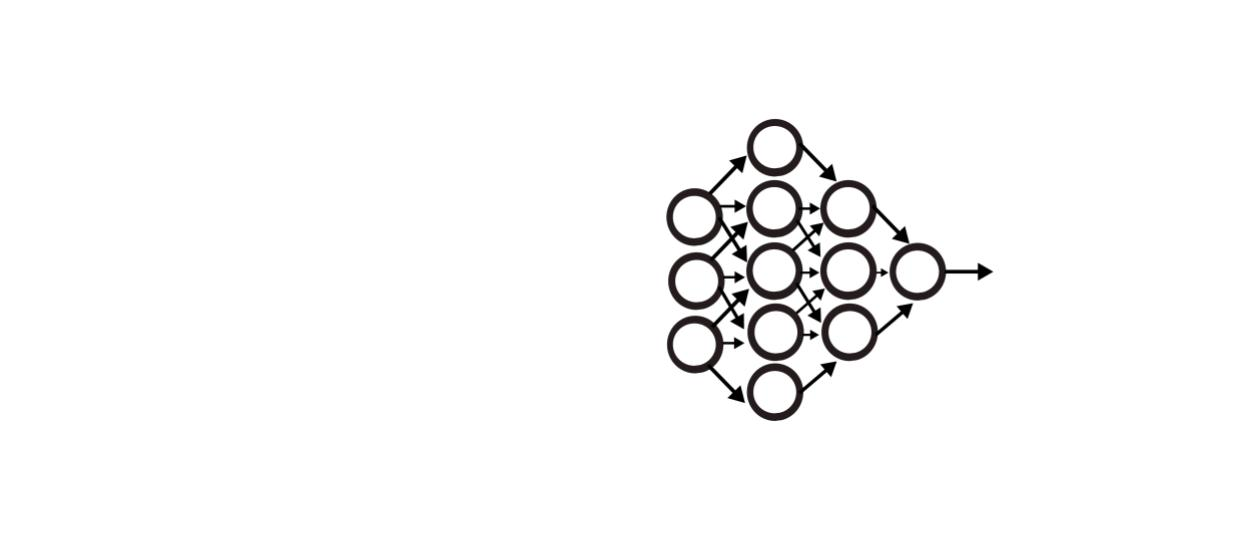
\includegraphics[width=1.2\textwidth]{figures/tl_}
	\end{figure}
	 
\end{frame}

\begin{frame}{On the Transferability of Convolutional Neural Networks}
	\bigskip

	\begin{figure}
		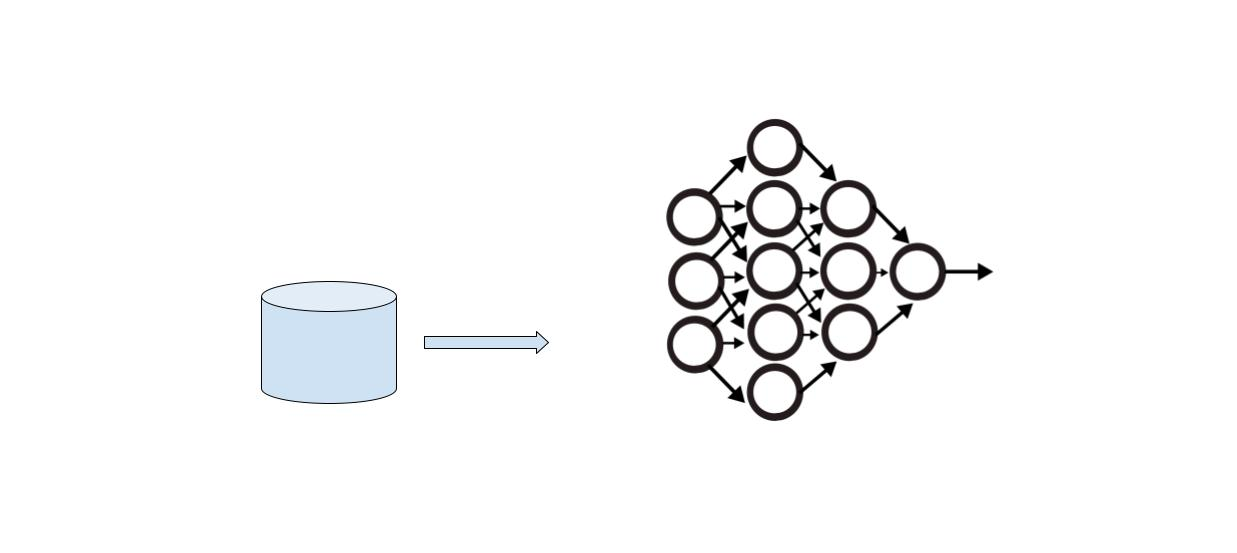
\includegraphics[width=1.2\textwidth]{figures/tl__}
	\end{figure}
	 
\end{frame}

\begin{frame}{On the Transferability of Convolutional Neural Networks}
	\bigskip

	\begin{figure}
		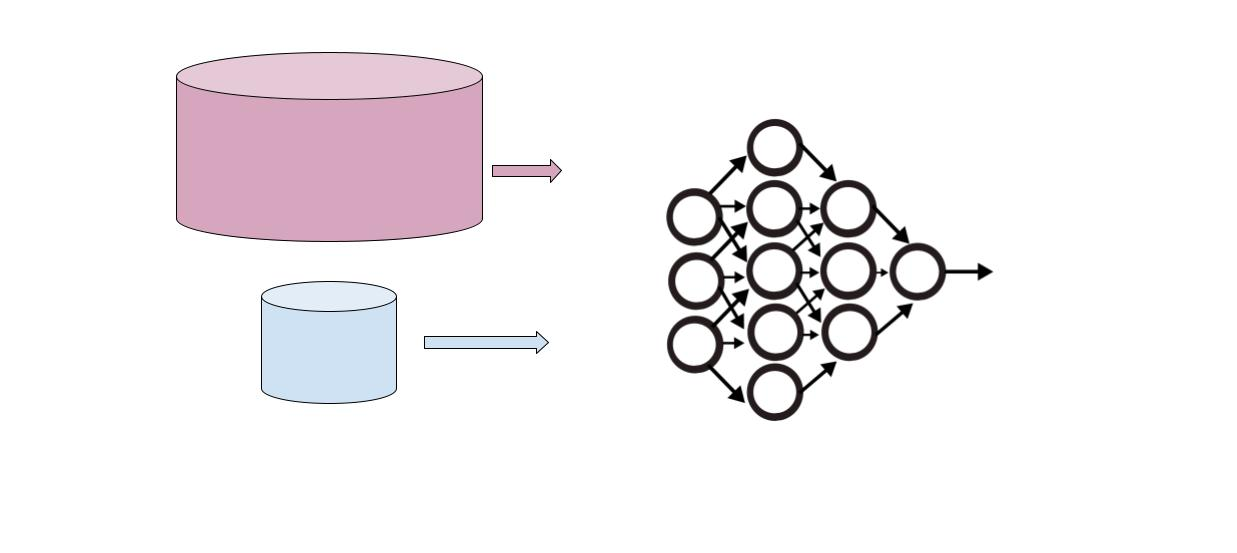
\includegraphics[width=1.2\textwidth]{figures/tl___}
	\end{figure}
	 
\end{frame}


\iffalse
\begin{frame}{On the Transferability of Convolutional Neural Networks}

	For our first study ...
	\bigskip
	\begin{itemize}
		\item We consider $f$ to come in the form of a \textcolor{RoyalBlue}{Convolutional Neural Network} (CNN)
		\item We define the source domain $\mathcal{D}_S$ to be that of \textcolor{RoyalBlue}{natural images}
		\item We define the target domain $\mathcal{D}_T$ to be that of \textcolor{RoyalBlue}{Digital Heritage}
		\item We assume that labels are available in both the source and target data and that the input spaces ${\cal X}_T$ and ${\cal X}_S$ match: \textcolor{RoyalBlue}{Inductive Transfer Learning}
	\end{itemize}

\end{frame}
\fi

\begin{frame}{On the Transferability of Convolutional Neural Networks}

	\begin{columns}
		\begin{column}{.5\textwidth}
			As source-task $\mathcal{T}_S$ we have a CNN pre-trained on the ImageNet dataset

			\begin{figure}
				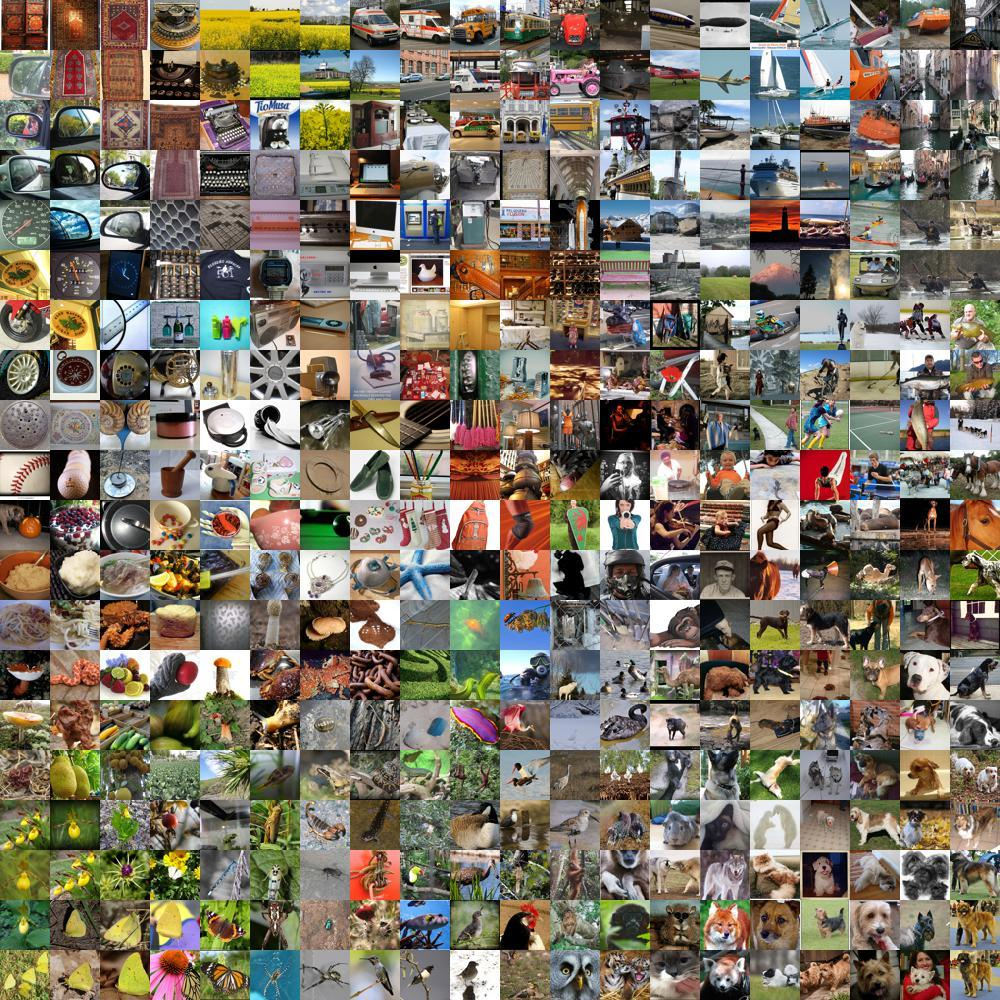
\includegraphics[width=0.8\textwidth]{figures/imagenet}
			\end{figure}

		\end{column}
		
		\begin{column}{.5\textwidth}
			We have three target-tasks $\mathcal{T}_T$ defined by the Rijksmuseum collection

			\begin{figure}
				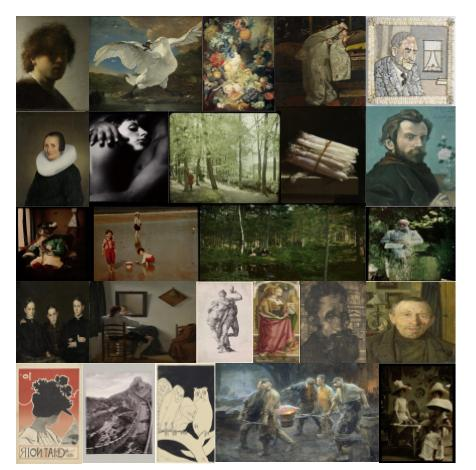
\includegraphics[width=0.85\textwidth]{figures/rijks}
			\end{figure}

		\end{column}
		
	\end{columns}

\end{frame}


\begin{frame}{On the Transferability of Convolutional Neural Networks}

	More specifically we aim to classify the artworks of the Rijksmuseum by:
	\bigskip

	\begin{columns}
		\begin{column}{.3\textwidth}
			\textcolor{RoyalBlue}{Material}: $\mathcal{T}_T$ \circled{1}
			\begin{figure}
				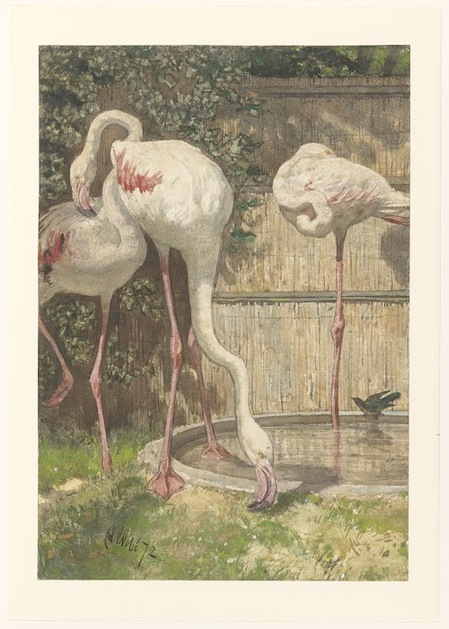
\includegraphics[width=0.9\textwidth]{figures/paper}
			\end{figure}
		\end{column}
		
		\begin{column}{.3\textwidth}
			\textcolor{RoyalBlue}{Type}: $\mathcal{T}_T$ \circled{2}
			\begin{figure}
				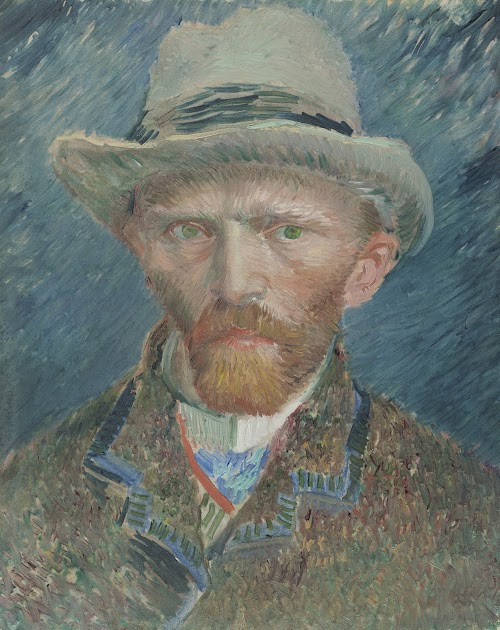
\includegraphics[width=1\textwidth]{figures/portrait}
			\end{figure}
		\end{column}
			
		\begin{column}{.3\textwidth}
			\textcolor{RoyalBlue}{Artist}: $\mathcal{T}_T$ \circled{3}
			\begin{figure}
				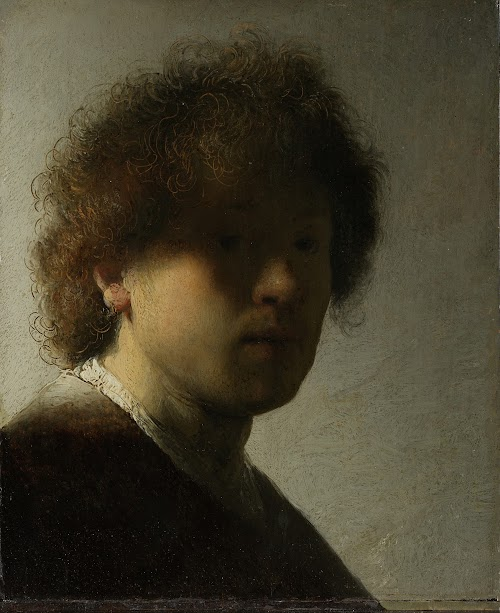
\includegraphics[width=1\textwidth]{figures/rembrandt}
			\end{figure}
		\end{column}
		
	\end{columns}

\end{frame}


\begin{frame}{On the Transferability of Convolutional Neural Networks}

	\begin{table}[ht!]
\scriptsize
\centering
\caption{An overview of the two datasets that are used in our experiments. For each heritage collection we report with $N_t$ the amount of samples constituting the datasets and with $Q_t$ the number of labels. Lastly, we also report if there are common labels between the two heritage collections.}
\begin{tabular}{c|c|c|c|c} 
	\hline
	$\mathcal{T}_T$ & Dataset & \textbf{$N_t$} & \textbf{$Q_t$} & $\%$ of overlap \\\hline \hline
        Material \circled{1} & Rijksmuseum  & $110,668$ & $206$ &  $\varnothing$ \\ 
         & Antwerp & $-$ & $-$    \\
        Type \circled{2} & Rijksmuseum  & $112,012$ & $1,054$   \\
         & Antwerp & $23,797$ & $920$ & $\approx 15\%$ \\
        Artist \circled{3} & Rijksmuseum & $82,018$ & $1,196$  & $\varnothing$ \\ 
         & Antwerp  & $18,656$ & $903$ \\        
	\hline
\end{tabular}
\label{table:dataset_overview}
\end{table}   

	\bigskip
	$\Rightarrow$ Experimental setup ...
	\begin{itemize}
		\item We compare the transfer learning performance of four CNN architectures 
		\item Explore three training strategies
	\end{itemize}
\end{frame}

\begin{frame}{On the Transferability of Convolutional Neural Networks}
	
	\bigskip

	\begin{itemize}
		\item Let us consider a simplified neural network
	\end{itemize}

	\bigskip

	\begin{figure}
		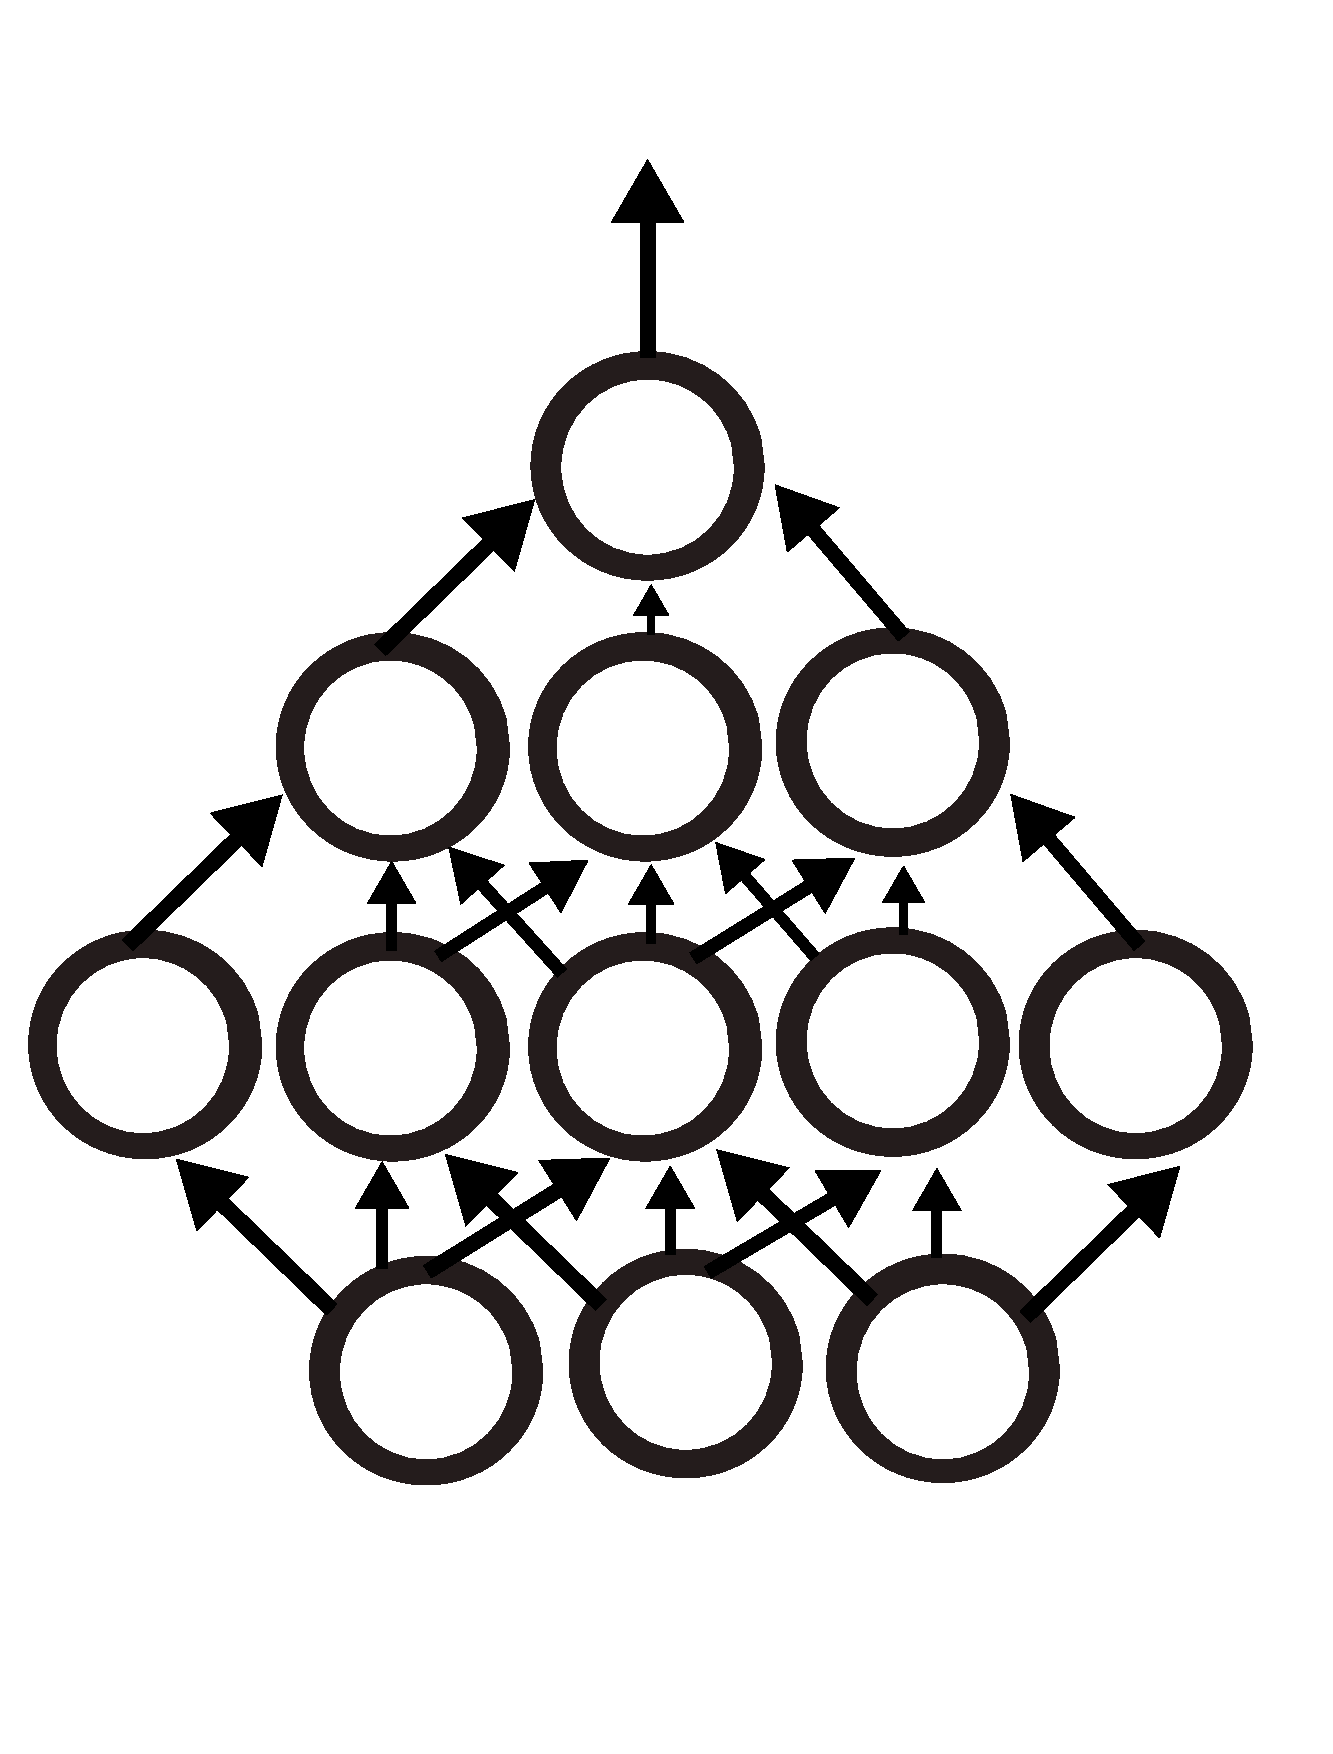
\includegraphics[width=0.5\textwidth]{figures/mlp.pdf}
	\end{figure}

\end{frame}


\iffalse
\begin{frame}{On the Transferability of Convolutional Neural Networks}
	
	\bigskip

	\begin{itemize}
		\item A \textcolor{RoyalBlue}{randomly} initialized model
	\end{itemize}

	\bigskip

	\begin{figure}
		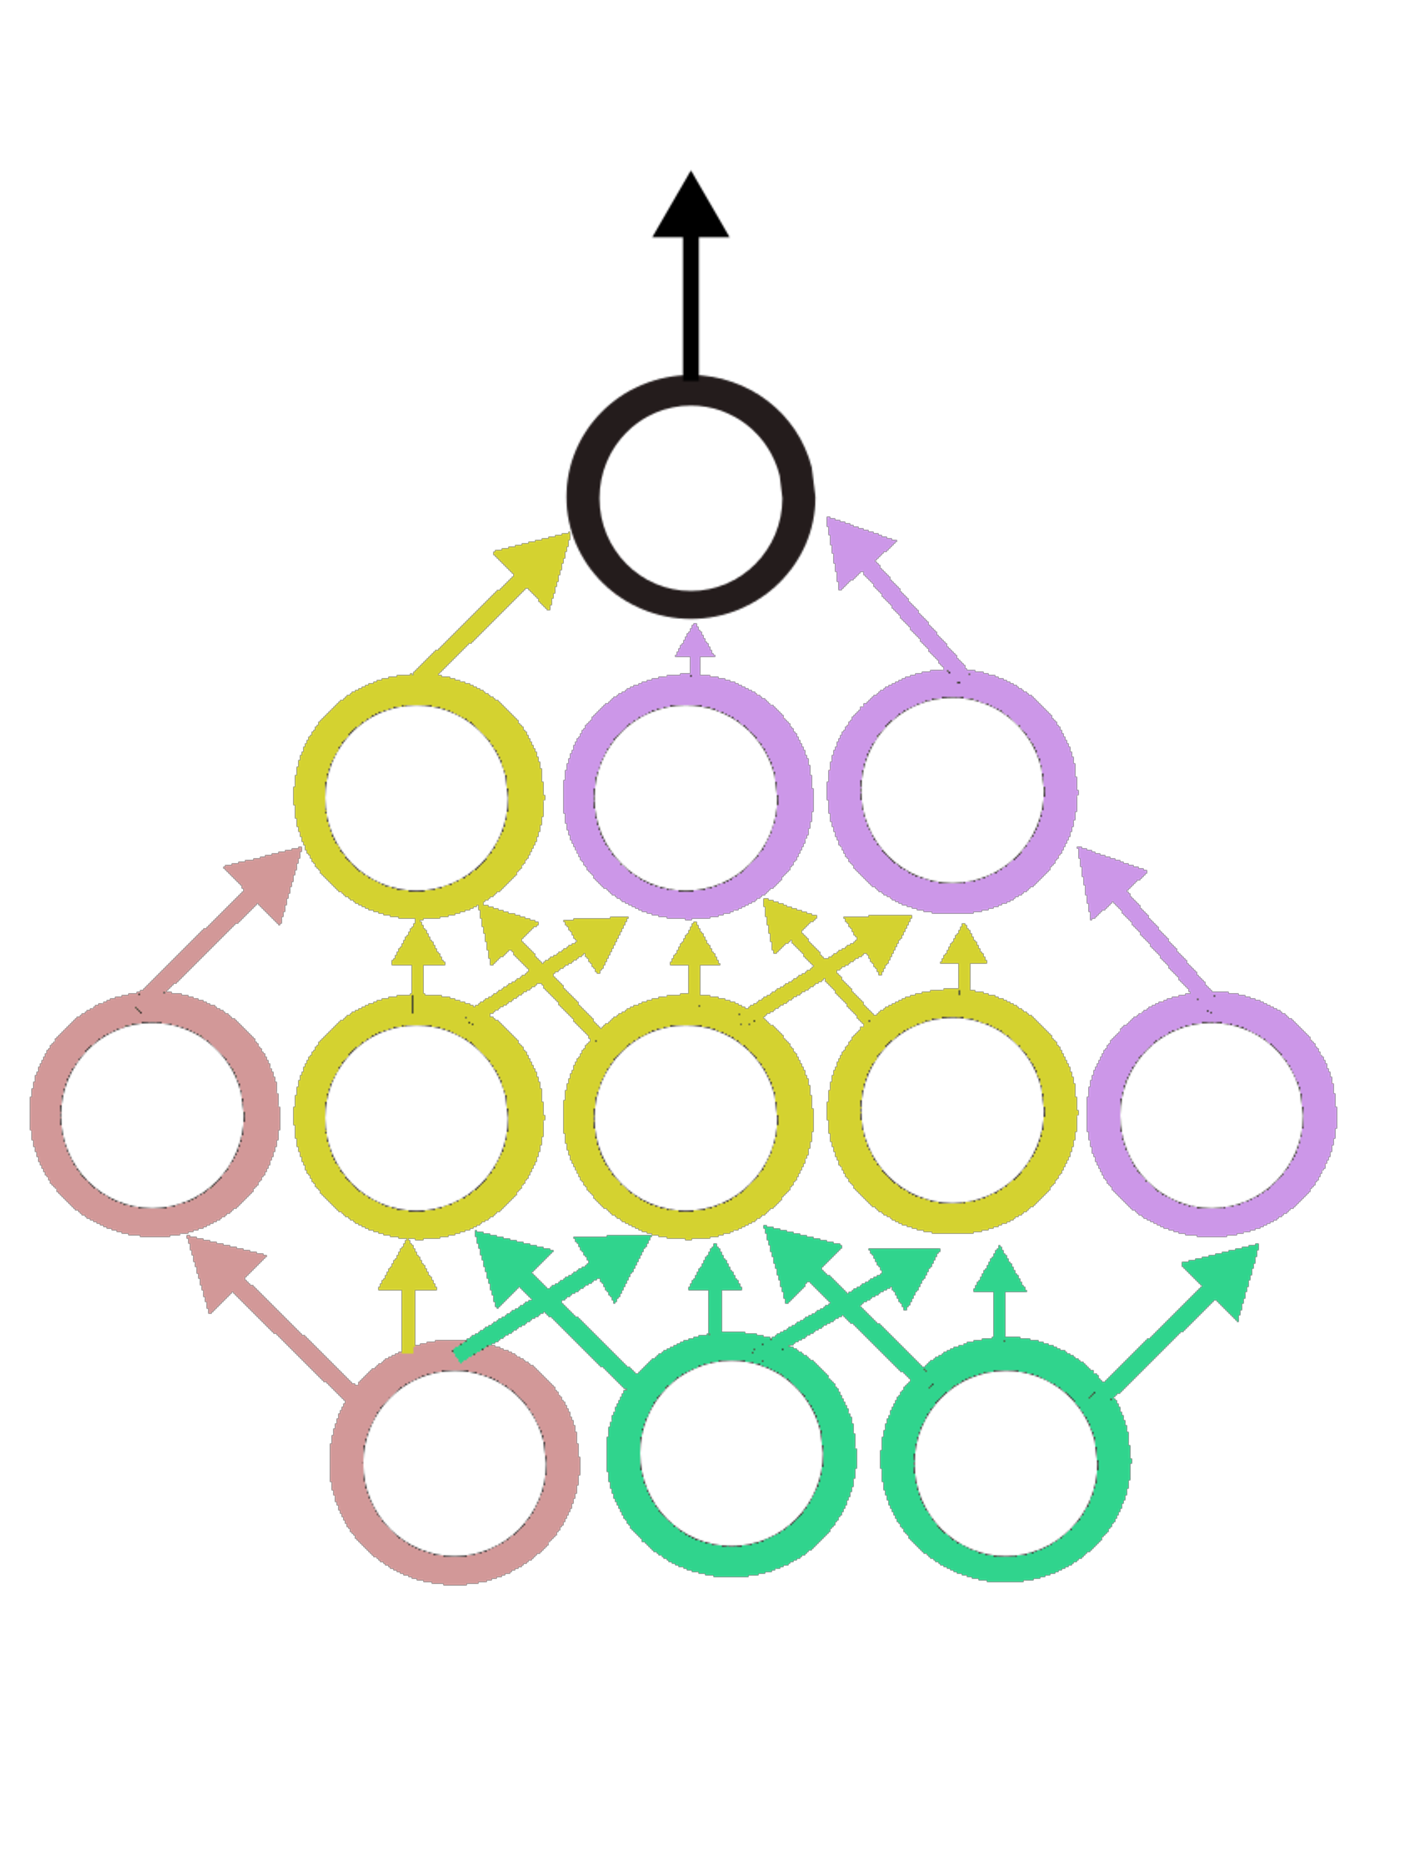
\includegraphics[width=0.5\textwidth]{figures/random_net.pdf}
	\end{figure}

\end{frame}
\fi


\begin{frame}{On the Transferability of Convolutional Neural Networks}
	
	\bigskip

	\begin{itemize}
		\item The \textcolor{RoyalBlue}{off-the-shelf} approach 
	\end{itemize}

	\bigskip

	\begin{figure}
		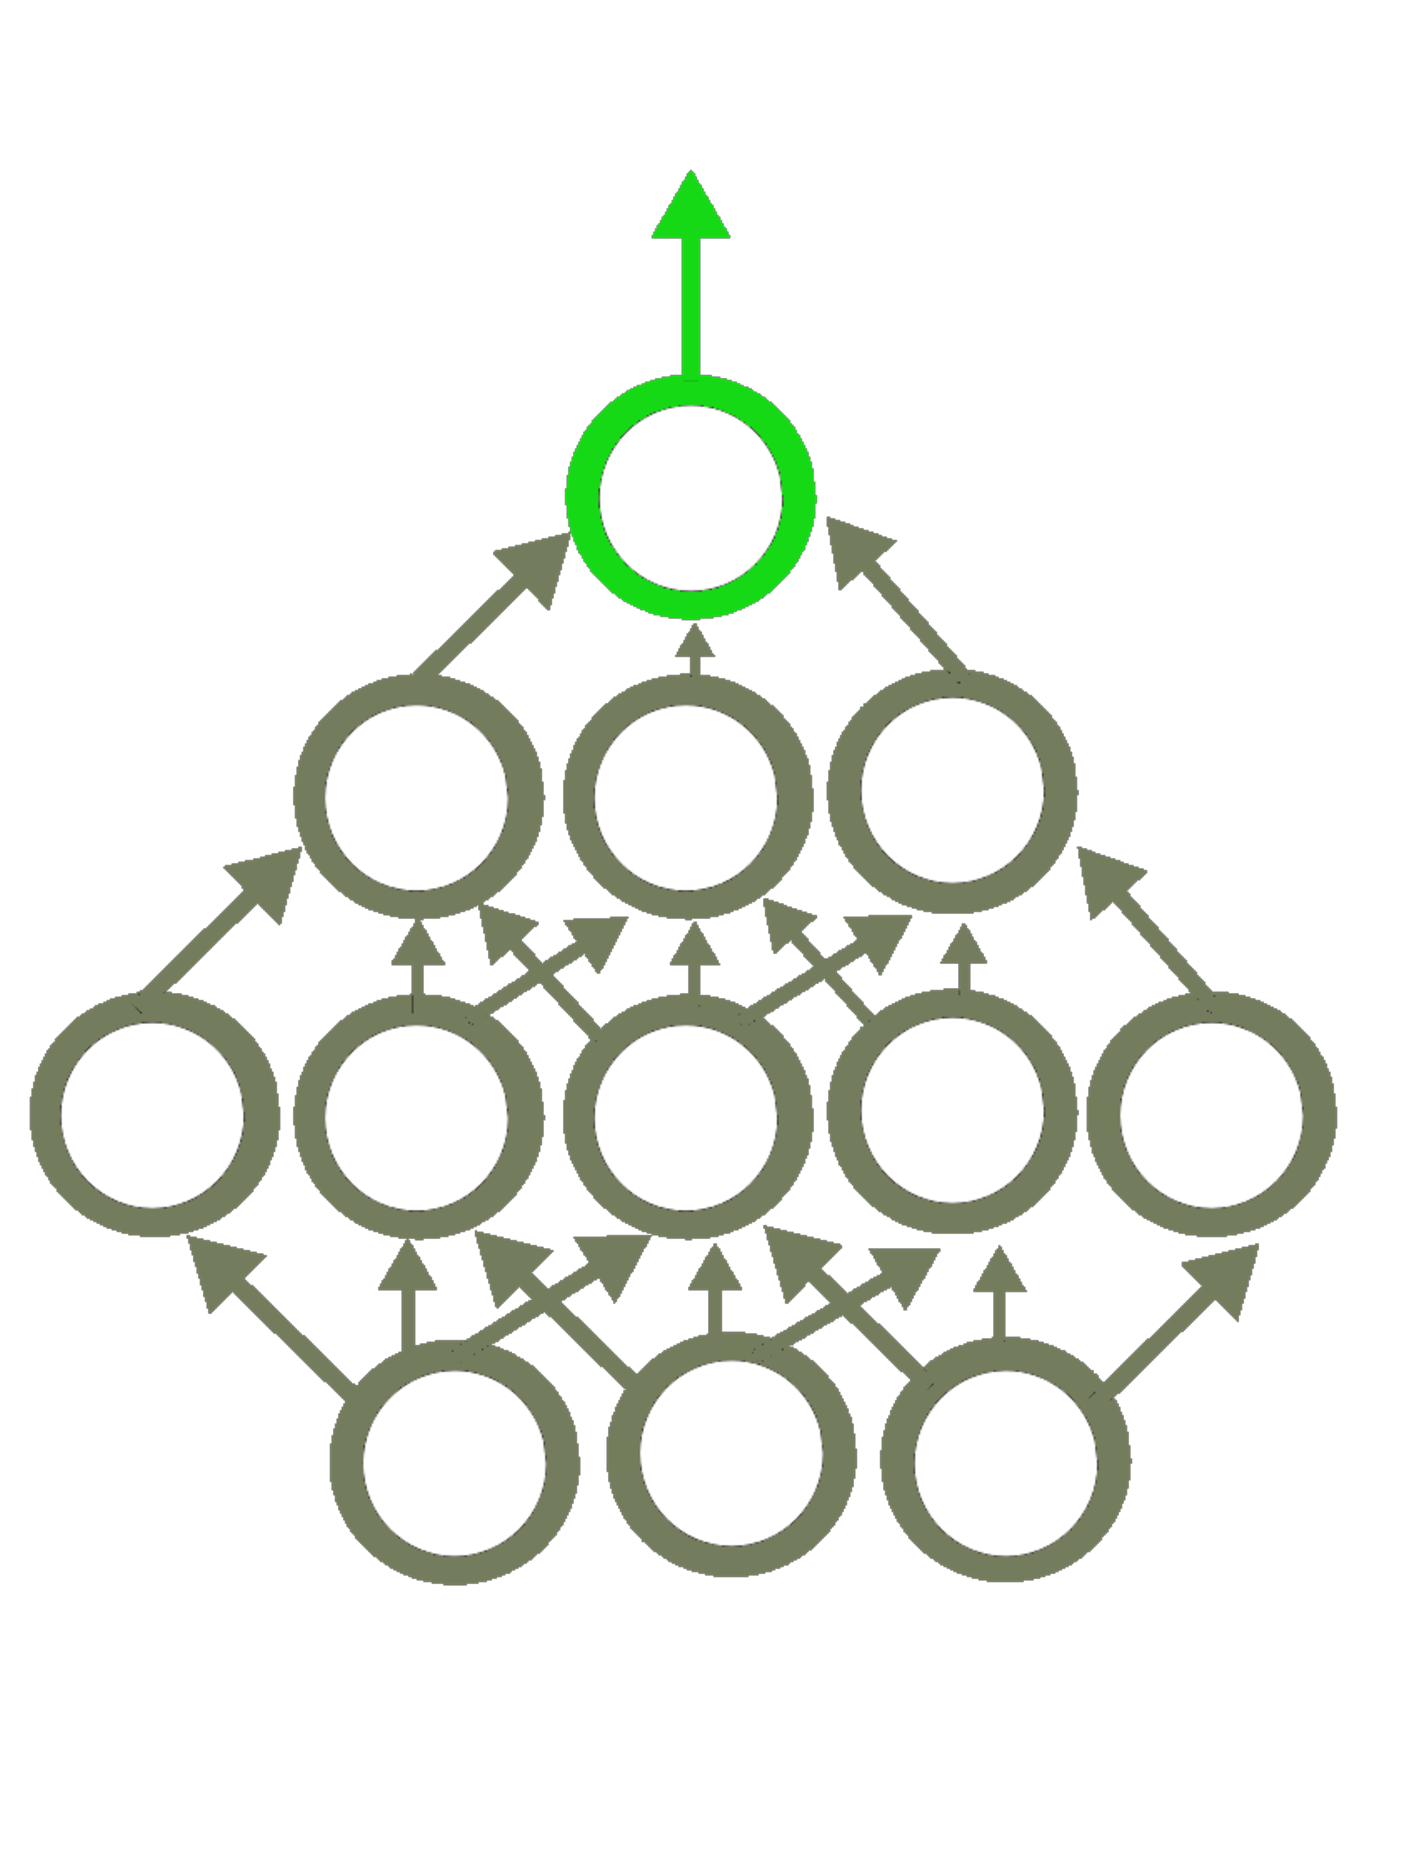
\includegraphics[width=0.5\textwidth]{figures/frozen_net.pdf}
	\end{figure}

\end{frame}


\begin{frame}{On the Transferability of Convolutional Neural Networks}
	
	\bigskip

	\begin{itemize}
		\item The \textcolor{RoyalBlue}{fine-tuning} approach 
	\end{itemize}

	\bigskip

	\begin{figure}
		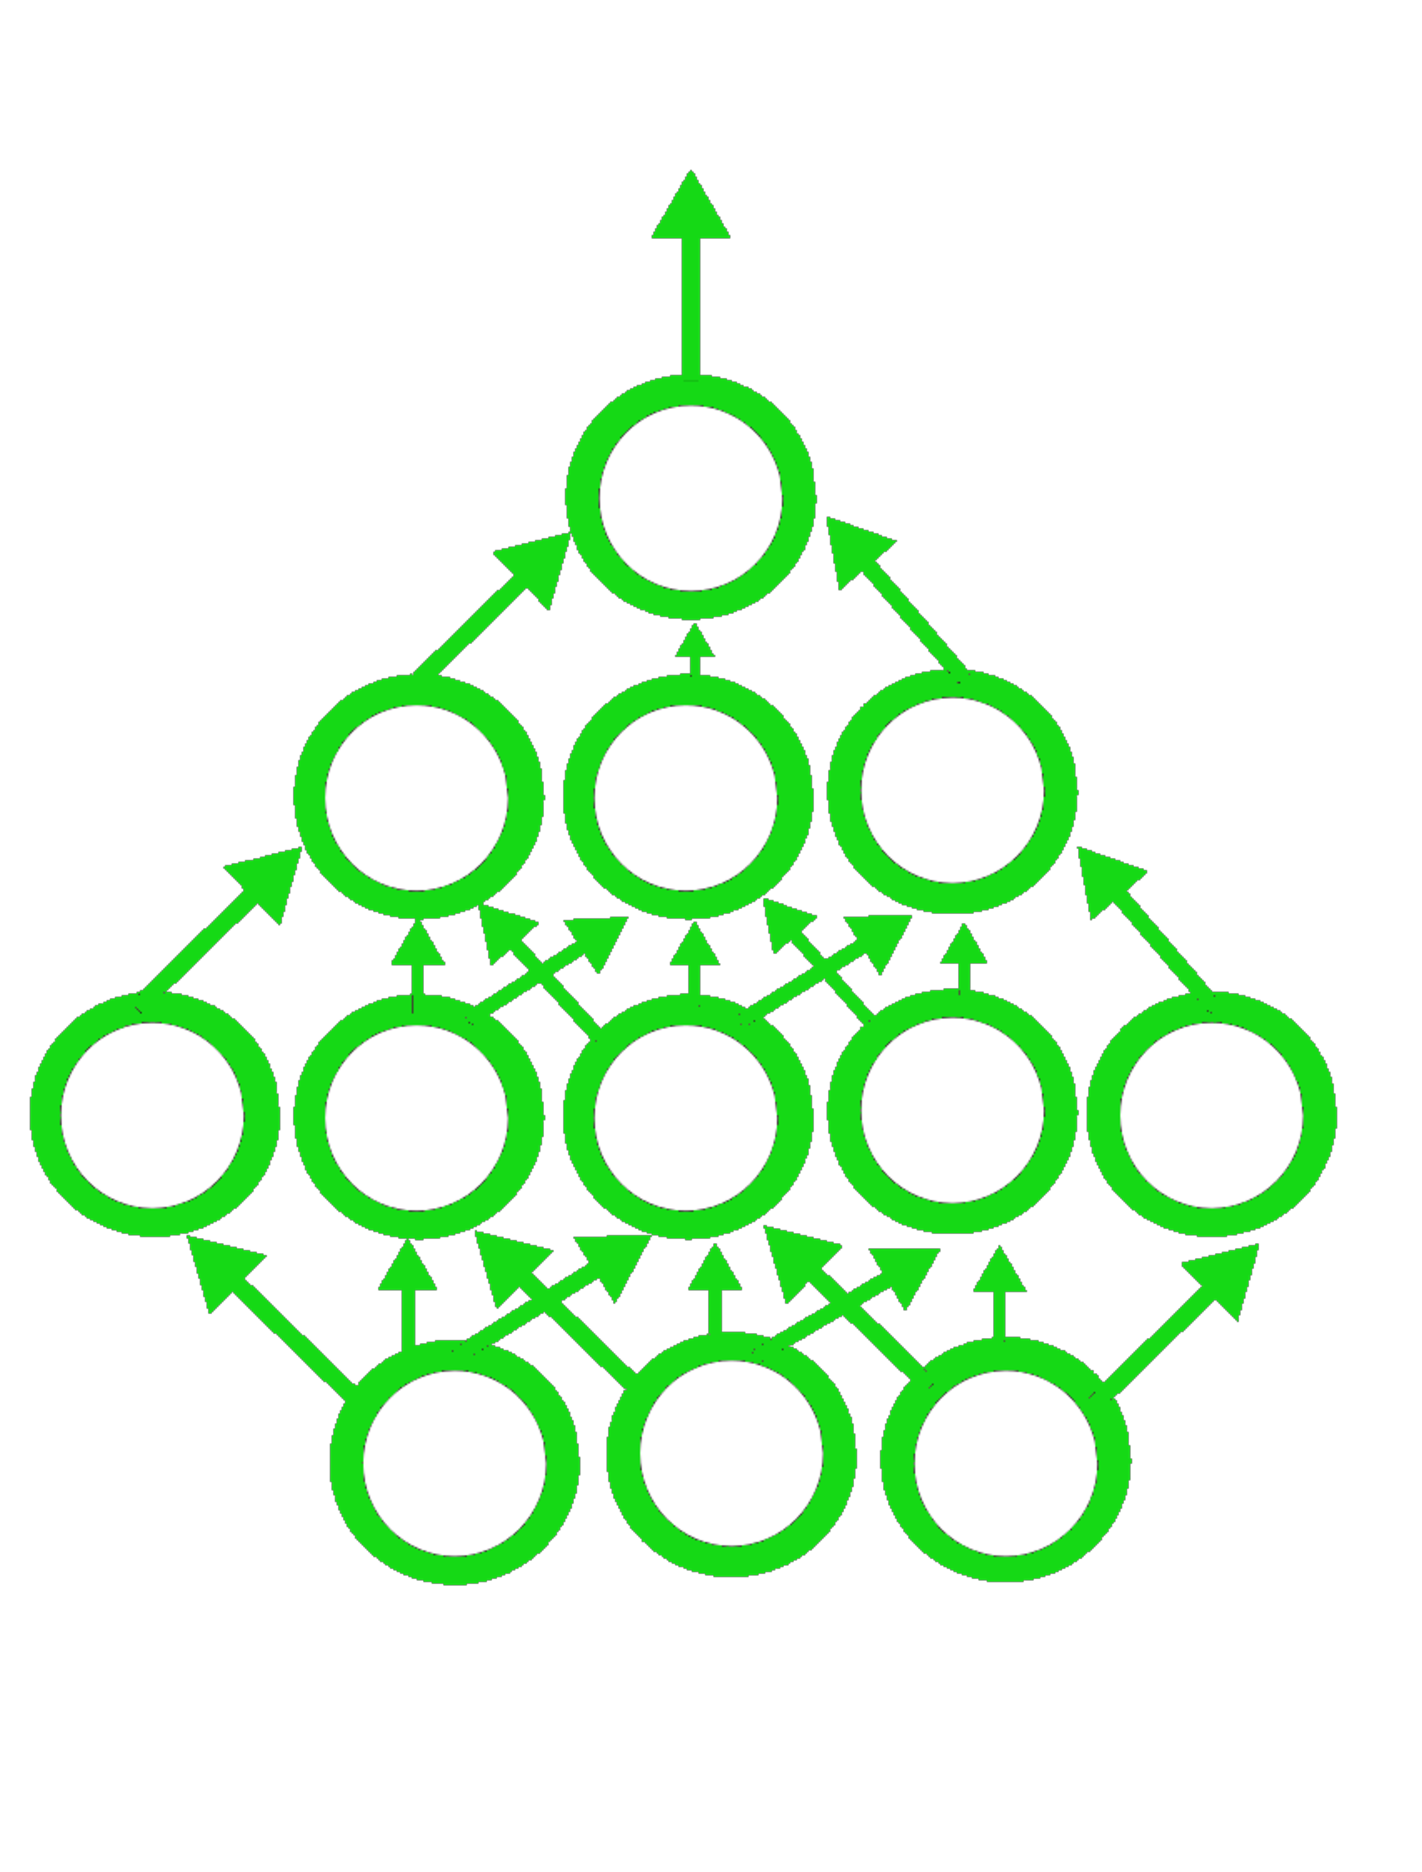
\includegraphics[width=0.5\textwidth]{figures/fine_tuning_net.pdf}
	\end{figure}

\end{frame}


\begin{frame}{On the Transferability of Convolutional Neural Networks}
	\bigskip
	The performance on $\mathcal{T}_T$ \circled{1}
	
	\begin{figure}[ht]
  \centering
  \begin{tikzpicture}[scale = 0.8]

\begin{axis}[
	grid style={dashed,gray},
	grid = both, 
	tick style=black,
  	xlabel=Epochs,
  	ylabel= Accuracy ($\%$),
	title=$\mathcal{T}_T$ \circled{1},
	%width=1,
    	xmin=0,
    	xmax=10,
    	ymin=0.80,
    	ymax=0.95,
  	legend pos=outer north east,
]
	%\addlegendentry{Xception $\theta_{i}$}
	%\addlegendentry{ResNet50 $\theta_{i}$}
	%\addlegendentry{InceptionV3 $\theta_{i}$}
	%\addlegendentry{VGG19 $\theta_{i}$}      	
	\addlegendentry{Scratch-V3 $\theta$}	      	
	%\addlegendentry{Xception $\theta^{-}_{i}$}
      	%\addlegendentry{ResNet50 $\theta^{-}_{i}$}
      	%\addlegendentry{InceptionV3 $\theta^{-}_{i}$}
      	%\addlegendentry{VGG19 $\theta^{-}_{i}$}


%\addplot [thick, blue, mark=x] table [y=Xception, x=epochs]{./Chapter04/logs/res_1.txt};
%\addplot [thick, red, mark=x] table [y=ResNet, x=epochs]{./Chapter04/logs/res_1.txt};
%\addplot [thick, black, mark=x] table [y=V3, x=epochs]{./Chapter04/logs/res_1.txt};
%\addplot [thick, green, mark=x] table [y=VGG19, x=epochs]{./Chapter04/logs/res_1.txt};
\addplot [ultra thick, orange, solid] table [y=RandomV3, x=epochs]{./Chapter04/logs/res_1.txt};


%\addplot [thick, blue, mark=halfcircle] table [y=Xception, x=epochs]{./Chapter04/logs/res_2.txt};
%\addplot [thick, red, mark=halfcircle] table [y=ResNet, x=epochs]{./Chapter04/logs/res_2.txt};
%\addplot [thick, black, mark=halfcircle] table [y=V3, x=epochs]{./Chapter04/logs/res_2.txt};
%\addplot [thick, green, mark=halfcircle] table [y=VGG19, x=epochs]{./Chapter04/logs/res_2.txt};



\end{axis}
    \end{tikzpicture}
\end{figure} 

\end{frame}

\begin{frame}{On the Transferability of Convolutional Neural Networks}
	\bigskip
	The performance on $\mathcal{T}_T$ \circled{1}
	
	\begin{figure}[ht]
  \centering
  \begin{tikzpicture}[scale = 0.8]

\begin{axis}[
	grid style={dashed,gray},
	grid = both, 
	tick style=black,
  	xlabel=Epochs,
  	ylabel= Accuracy ($\%$),
	title=$\mathcal{T}_T$ \circled{1},
	%width=1,
    	xmin=0,
    	xmax=10,
    	ymin=0.80,
    	ymax=0.95,
  	legend pos=outer north east,
]
	%\addlegendentry{Xception $\theta_{i}$}
	%\addlegendentry{ResNet50 $\theta_{i}$}
	%\addlegendentry{InceptionV3 $\theta_{i}$}
	%\addlegendentry{VGG19 $\theta_{i}$}      	
	\addlegendentry{Scratch-V3 $\theta$}	      	
	\addlegendentry{Xception $\theta^{-}_{i}$}
      	\addlegendentry{ResNet50 $\theta^{-}_{i}$}
      	\addlegendentry{InceptionV3 $\theta^{-}_{i}$}
      	\addlegendentry{VGG19 $\theta^{-}_{i}$}


%\addplot [thick, blue, mark=x] table [y=Xception, x=epochs]{./Chapter04/logs/res_1.txt};
%\addplot [thick, red, mark=x] table [y=ResNet, x=epochs]{./Chapter04/logs/res_1.txt};
%\addplot [thick, black, mark=x] table [y=V3, x=epochs]{./Chapter04/logs/res_1.txt};
%\addplot [thick, green, mark=x] table [y=VGG19, x=epochs]{./Chapter04/logs/res_1.txt};
\addplot [ultra thick, orange, solid] table [y=RandomV3, x=epochs]{./Chapter04/logs/res_1.txt};


\addplot [thick, blue, mark=halfcircle] table [y=Xception, x=epochs]{./Chapter04/logs/res_2.txt};
\addplot [thick, red, mark=halfcircle] table [y=ResNet, x=epochs]{./Chapter04/logs/res_2.txt};
\addplot [thick, black, mark=halfcircle] table [y=V3, x=epochs]{./Chapter04/logs/res_2.txt};
\addplot [thick, green, mark=halfcircle] table [y=VGG19, x=epochs]{./Chapter04/logs/res_2.txt};



\end{axis}
    \end{tikzpicture}
\end{figure} 

\end{frame}

\begin{frame}{On the Transferability of Convolutional Neural Networks}
	\bigskip
	The performance on $\mathcal{T}_T$ \circled{1}
	
	\begin{figure}[ht]
  \centering
  \begin{tikzpicture}[scale = 0.8]

\begin{axis}[
	grid style={dashed,gray},
	grid = both, 
	tick style=black,
  	xlabel=Epochs,
  	ylabel= Accuracy ($\%$),
	title=$\mathcal{T}_T$ \circled{1},
	%width=1,
    	xmin=0,
    	xmax=10,
    	ymin=0.80,
    	ymax=0.95,
  	legend pos=outer north east,
]
	\addlegendentry{Xception $\theta_{i}$}
	\addlegendentry{ResNet50 $\theta_{i}$}
	\addlegendentry{InceptionV3 $\theta_{i}$}
	\addlegendentry{VGG19 $\theta_{i}$}      	
	\addlegendentry{Scratch-V3 $\theta$}	      	
	\addlegendentry{Xception $\theta^{-}_{i}$}
      	\addlegendentry{ResNet50 $\theta^{-}_{i}$}
      	\addlegendentry{InceptionV3 $\theta^{-}_{i}$}
      	\addlegendentry{VGG19 $\theta^{-}_{i}$}


\addplot [thick, blue, mark=x] table [y=Xception, x=epochs]{./Chapter04/logs/res_1.txt};
\addplot [thick, red, mark=x] table [y=ResNet, x=epochs]{./Chapter04/logs/res_1.txt};
\addplot [thick, black, mark=x] table [y=V3, x=epochs]{./Chapter04/logs/res_1.txt};
\addplot [thick, green, mark=x] table [y=VGG19, x=epochs]{./Chapter04/logs/res_1.txt};
\addplot [ultra thick, orange, solid] table [y=RandomV3, x=epochs]{./Chapter04/logs/res_1.txt};


\addplot [thick, blue, mark=halfcircle] table [y=Xception, x=epochs]{./Chapter04/logs/res_2.txt};
\addplot [thick, red, mark=halfcircle] table [y=ResNet, x=epochs]{./Chapter04/logs/res_2.txt};
\addplot [thick, black, mark=halfcircle] table [y=V3, x=epochs]{./Chapter04/logs/res_2.txt};
\addplot [thick, green, mark=halfcircle] table [y=VGG19, x=epochs]{./Chapter04/logs/res_2.txt};



\end{axis}
    \end{tikzpicture}
\end{figure} 

\end{frame}

\begin{frame}{On the Transferability of Convolutional Neural Networks}
	\bigskip
	The performance on $\mathcal{T}_T$ \circled{2} and $\mathcal{T}_T$ \circled{3}

	\begin{figure}[ht!]
  \begin{tikzpicture}[scale = 0.55]
      \begin{axis}[
	name=ax1,
      	grid style={dashed,gray},
      	grid = both, 
      	tick style=black,
	title=$\mathcal{T}_T$ \circled{2},
        xlabel=Epochs,
        ylabel= Accuracy ($\%$),
	ymin=0.65,
      ]


      \addlegendentry{Xception $\theta^{-}_{i}$}
      \addlegendentry{ResNet50 $\theta^{-}_{i}$}
      \addlegendentry{InceptionV3 $\theta^{-}_{i}$}
      \addlegendentry{VGG19 $\theta^{-}_{i}$}
	\addlegendentry{Scratch-V3 $\theta$}
	\addlegendentry{Xception $\theta_{i}$}
	\addlegendentry{ResNet50 $\theta_{i}$}
	\addlegendentry{InceptionV3 $\theta_{i}$}
	\addlegendentry{VGG19 $\theta_{i}$}

      \addplot [thick, blue, mark=diamond] table [y=Xception, x=epochs]
      {./Chapter04/logs/rijksmuseum_type_challenge_only_softmax.txt};
      \addplot [thick, red, mark=diamond] table [y=ResNet, x=epochs]{./Chapter04/logs/rijksmuseum_type_challenge_only_softmax.txt};
      \addplot [thick, black, mark=diamond] table [y=V3, x=epochs]{./Chapter04/logs/rijksmuseum_type_challenge_only_softmax.txt};
      \addplot [thick, green, mark=diamond] table [y=VGG19, x=epochs]{./Chapter04/logs/rijksmuseum_type_challenge_only_softmax.txt};
            \addplot [ultra thick, orange , solid] table [y=ScratchV3, x=epochs]{./Chapter04/logs/rijksmuseum_type_challenge_full_fine_tuning.txt};

      \addplot [ thick, blue, mark=x] table [y=Xception, x=epochs]{./Chapter04/logs/rijksmuseum_type_challenge_full_fine_tuning.txt};
      \addplot [ thick, red, mark=x] table [y=ResNet, x=epochs]{./Chapter04/logs/rijksmuseum_type_challenge_full_fine_tuning.txt};
      \addplot [thick, black, mark=x] table [y=V3, x=epochs]{./Chapter04/logs/rijksmuseum_type_challenge_full_fine_tuning.txt};
      \addplot [thick, green, mark=x] table [y=VGG19, x=epochs]{./Chapter04/logs/rijksmuseum_type_challenge_full_fine_tuning.txt};

\legend{}

      \end{axis}

      \begin{axis}[
	at={(ax1.south east)},
	xshift=2cm,
      	grid style={dashed,gray},
      	grid = both, 
      	tick style=black,
	title=$\mathcal{T}_T$ \circled{3},
        xlabel=Epochs,
        ylabel= Accuracy ($\%$),
	legend columns=3, 
        legend style={font=\small, at={(-0.8,-0.2,-0.2)},anchor=north west,legend columns=3},
      ]


      \addlegendentry{Xception $\theta^{-}_{i}$}
      \addlegendentry{ResNet50 $\theta^{-}_{i}$}
      \addlegendentry{InceptionV3 $\theta^{-}_{i}$}
      \addlegendentry{VGG19 $\theta^{-}_{i}$}
	\addlegendentry{Scratch-V3 $\theta$}
	\addlegendentry{Xception $\theta_{i}$}
	\addlegendentry{ResNet50 $\theta_{i}$}
	\addlegendentry{InceptionV3 $\theta_{i}$}
	\addlegendentry{VGG19 $\theta_{i}$}



      \addplot [thick, blue, mark=diamond] table [y=Xception, x=epochs]
      {./Chapter04/logs/rijksmuseum_artist_challenge_only_softmax.txt};
      \addplot [thick, red, mark=diamond] table [y=ResNet, x=epochs]{./Chapter04/logs/rijksmuseum_artist_challenge_only_softmax.txt};
      \addplot [thick, black, mark=diamond] table [y=V3, x=epochs]{./Chapter04/logs/rijksmuseum_artist_challenge_only_softmax.txt};
      \addplot [thick, green, mark=diamond] table [y=VGG19, x=epochs]{./Chapter04/logs/rijksmuseum_artist_challenge_only_softmax.txt};
            \addplot [ultra thick, orange , solid] table [y=ScratchV3, x=epochs]{./Chapter04/logs/rijksmuseum_artist_challenge_full_fine_tuning.txt};

      \addplot [ thick, blue, mark=x] table [y=Xception, x=epochs]{./Chapter04/logs/rijksmuseum_artist_challenge_full_fine_tuning.txt};
      \addplot [ thick, red, mark=x] table [y=ResNet, x=epochs]{./Chapter04/logs/rijksmuseum_artist_challenge_full_fine_tuning.txt};
      \addplot [thick, black, mark=x] table [y=V3, x=epochs]{./Chapter04/logs/rijksmuseum_artist_challenge_full_fine_tuning.txt};
      \addplot [thick, green, mark=x] table [y=VGG19, x=epochs]{./Chapter04/logs/rijksmuseum_artist_challenge_full_fine_tuning.txt};



      \end{axis}
	\end{tikzpicture}
\end{figure}


\end{frame}


\begin{frame}{On the Transferability of Convolutional Neural Networks}

	We observe that:
	\bigskip
	
	\begin{itemize}
		\item Both transfer learning approaches have significant \textcolor{RoyalBlue}{benefits} 
		\item The off-the-shelf approach performs \textcolor{RoyalBlue}{well} for  $\mathcal{T}_T$ \circled{1} and  $\mathcal{T}_T$ \circled{2} but \textcolor{Maroon}{fails} for  $\mathcal{T}_T$ \circled{3}
		\item Fine-tuning the networks results in \textcolor{RoyalBlue}{best} performance
	\end{itemize}

\end{frame}

\iffalse
\begin{frame}{On the Transferability of Convolutional Neural Networks}
	
	$\Rightarrow$ After having fine-tuned the ImageNet models on the Rijksmuseum collection we investigate whether these models \textcolor{RoyalBlue}{generalize} to different, smaller, artistic collections

	\bigskip

	\begin{itemize}
		\item We collected a new dataset of heritage objects present in the city of Antwerp
		\item Aim again at classifying their type $\mathcal{T}_T$ \circled{2} 
		\item And the respective artist $\mathcal{T}_T$ \circled{3}
		\item Compare the performance to ImageNet pre-trained models only
	\end{itemize}
	
\end{frame}

\begin{frame}{On the Transferability of Convolutional Neural Networks}

	
\begin{table}[ht]
	\caption{The results obtained on the classification experiments performed on the Antwerp dataset with models that have been initially pre-trained on ImageNet ($\theta^{i}$) and the same architectures which have been fine tuned on the Rijksmuseum dataset ($\theta^{r}$). Our results show that the latter pre-trained networks yield better results both if used as off the shelf feature extractors and if fine tuned.}
    \resizebox{\columnwidth}{!}{%
    \label{tab:Antwerpen_dataset}
    \centering
    \begin{tabular}{c|c|c|c|c|c}
	    $\mathcal{T}_T$ &model & $\theta^{i}$ + off the shelf & $\theta^{r}$ + off the shelf & $\theta^{i}$ + fine tuning & $\theta^{r}$ + fine tuning  \\
        \hline \hline
	\circled{2} & Xception  & 42.01\% &  \cellcolor{yellow!25}62.92\% &69.74\% & 72.03\%       \\
        \circled{2} & InceptionV3  & 43.90\% & 57.65\% &70.58\%  & 71.88\%    \\
	\circled{2} & ResNet50 & 41.59\% & \cellcolor{green!25}{64.95\%} & \cellcolor{yellow!25}76.50\% & \cellcolor{green!25}{78.15\%}    \\
        \circled{2} & VGG19 & 38.36\% & 60.10\%& 70.37\%  & 71.21\%      \\
        \hline
	\circled{3} & Xception  &48.52\% & \cellcolor{green!25}{54.81\%}& 58.15\% & 58.47\%   \\
        \circled{3} & InceptionV3 & 21.29\% &  53.41\%& 56.68\% & 57.84\%   \\
	\circled{3} & ResNet50 & 22.39\% & 31.38\% & \cellcolor{yellow!25}62.57\% & \cellcolor{green!25}{69.01\%}    \\
	\circled{3} & VGG19 &  49.90\% & \cellcolor{yellow!25}53.52\% & 54.90\% & 60.01\%  \\
        \end{tabular}%
}
\end{table}



\end{frame}
\fi

\begin{frame}{On the Transferability of Convolutional Neural Networks}

	\bigskip

	To conclude we show that
	
	\bigskip

	\begin{itemize}
		\item Modern Convolutional Neural Networks exhibit \textcolor{RoyalBlue}{strong transfer learning} potential
		\item Even when the source task $\mathcal{T}_S$ (natural images) and the target task are very different $\mathcal{T}_T$ (art classification)
		\item Best performance is obtained after fine-tuning, which however comes at a computational cost
	\end{itemize}

	\bigskip

	The present study only considers the computer vision task of \textcolor{RoyalBlue}{image classification} ...

\end{frame}

\begin{frame}{On the Transferability of Convolutional Neural Networks}
	\bigskip
	$\Rightarrow$ Which is a \textcolor{Maroon}{limitation} which we have addressed in our follow up work, where we perform a similar study for the computer vision task of \textcolor{RoyalBlue}{object detection}

	\bigskip
	
	For this purpose we have created the MINERVA dataset within the open-source \texttt{Cytomine} platform \footnote{Marée, Raphaël, et al. "Collaborative analysis of multi-gigapixel imaging data using Cytomine." Bioinformatics 32.9 (2016): 1395-1401.}

	\begin{figure}
		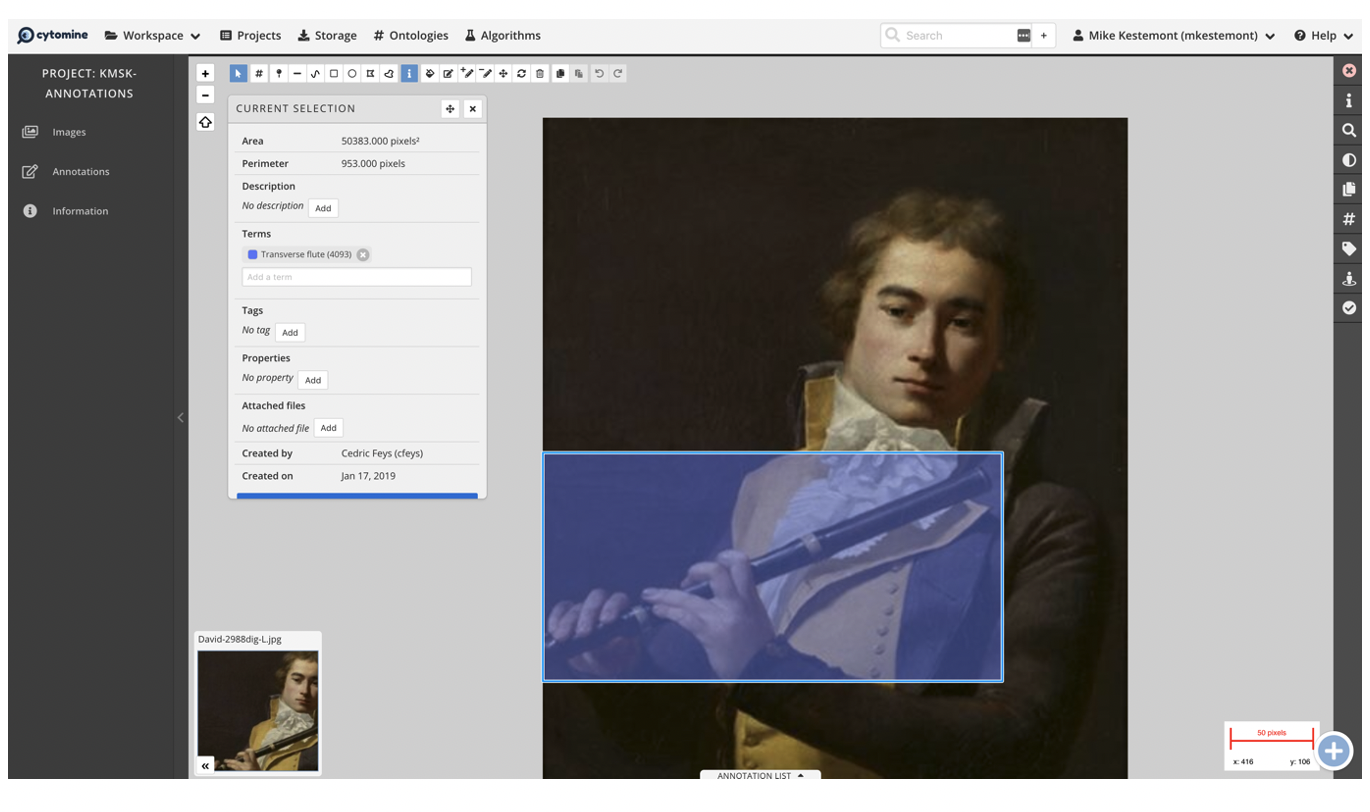
\includegraphics[width=0.6\textwidth]{figures/cytomine_annotations}
	\end{figure}

\end{frame}


\begin{frame}{On the Transferability of Convolutional Neural Networks}
	\bigskip
	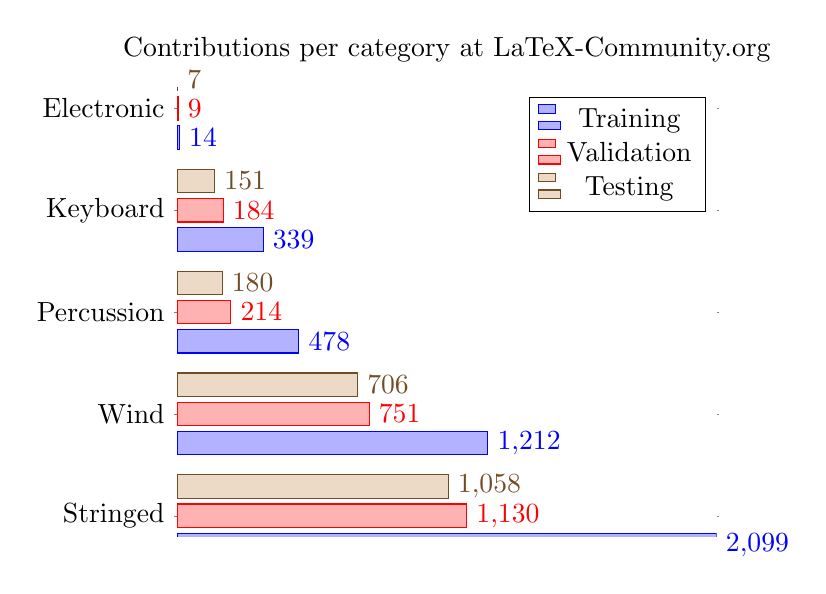
\begin{tikzpicture}
  \begin{axis}[title  = Contributions per category
                          at LaTeX-Community.org,
    xbar,
    bar width=.3cm,
    y axis line style = { opacity = 0 },
    axis x line       = none,
    tickwidth         = 1pt,
    enlarge y limits  = 0.05,
    enlarge x limits  = 0.001,
    symbolic y coords = {Stringed, Wind, Percussion,Keyboard, Electronic},
    nodes near coords,
  ]
\addplot coordinates {(2099,Stringed) (1212,Wind) (478,Percussion) (339,Keyboard) (14,Electronic)};
\addplot coordinates {(1130,Stringed) (751,Wind) (214,Percussion) (184,Keyboard) (9,Electronic)};
\addplot coordinates {(1058,Stringed) (706,Wind) (180,Percussion) (151,Keyboard) (7,Electronic)};
\legend{Training,Validation,Testing}

\end{axis}
\end{tikzpicture}

\iffalse
\end{axis}
\end{tikzpicture}
\fi

\end{frame}

\begin{frame}{On the Transferability of Convolutional Neural Networks}
	\begin{figure}
		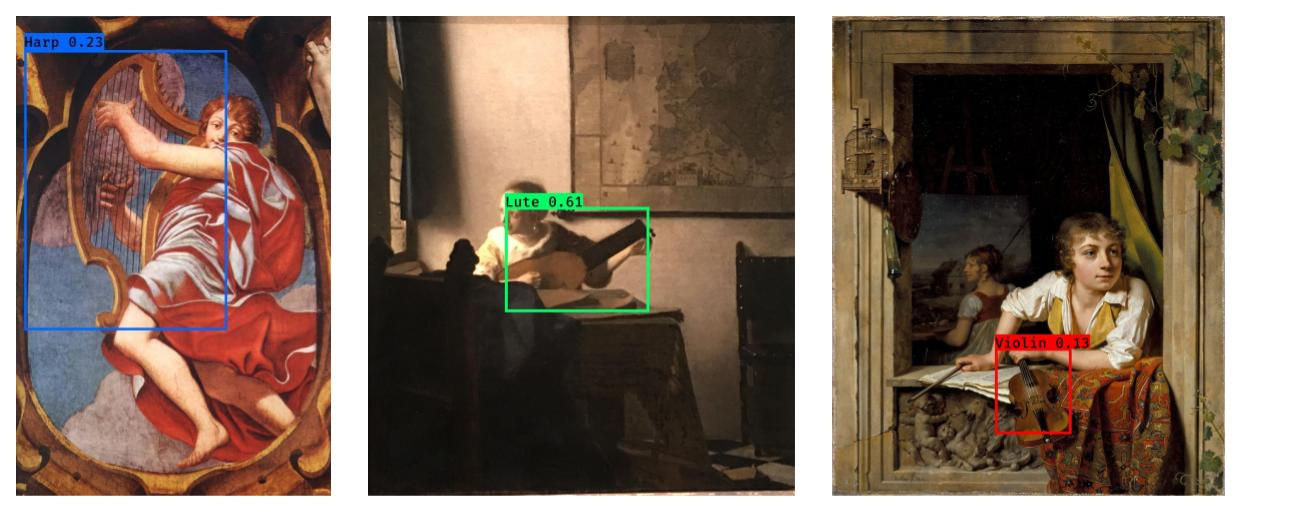
\includegraphics[width=1\textwidth]{figures/minerva}
	\end{figure}
\end{frame}


\begin{frame}{On the Transferability of Convolutional Neural Networks}
	
	In line with the classification experiments performed on the Rijksmuseum dataset, also when it comes to object detection we show that
	\bigskip
	\begin{itemize}
		\item Pre-trained object detectors \textcolor{RoyalBlue}{can get transferred} across domains 
		\item Fine-tuning these networks results in \textcolor{RoyalBlue}{best} performance
		\item This is the case for \textcolor{RoyalBlue}{different families} of object detection models ranging from YOLO, to networks that use region proposals and selective search \footnote{Claes, Yann. "Deep Learning for the Classification and Detection of Animals in Artworks." (2021).}.
	\end{itemize}

\end{frame}



\begin{frame}{On the Transferability of Lottery Winners}
	\subsection{On the Transferability of Lottery Winners}
\end{frame}


\begin{frame}{On the Transferability of Lottery Winners}

	\begin{center}
		\textcolor{RoyalBlue}{The Lottery Ticket Hypothesis}:
		\textit{"A randomly-initialized dense neural network contains a subnetwork that is initialized such that when trained in isolation it can match the test accuracy of the original network after training for at most the same number of iterations.\footnote{Frankle, Jonathan, and Michael Carbin. "The lottery ticket hypothesis: Finding sparse, trainable neural networks." (2018)}"}
	\end{center}

\end{frame}

\begin{frame}{On the Transferability of Lottery Winners}

	\begin{figure}
		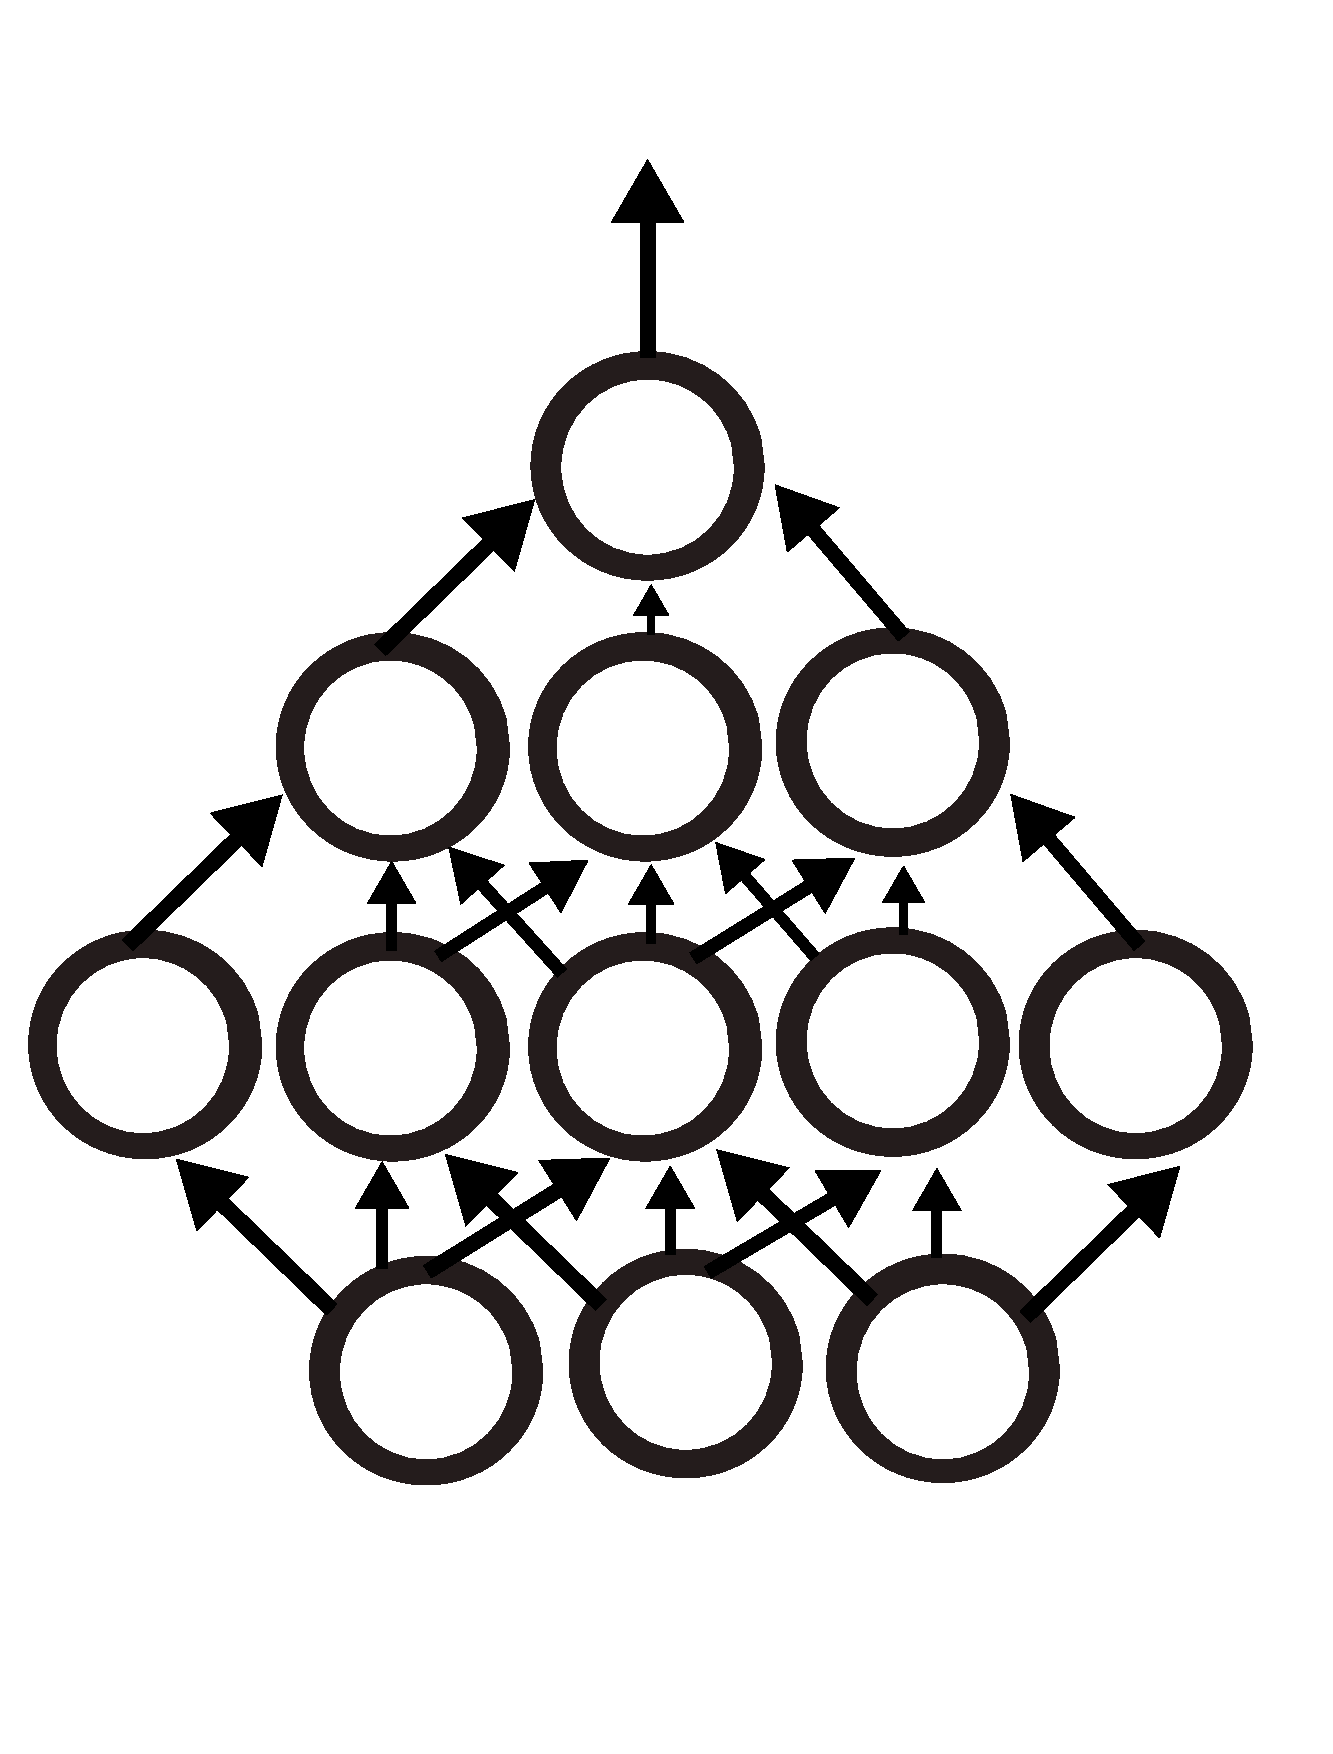
\includegraphics[width=0.5\textwidth]{figures/mlp.pdf}
	\end{figure}

\end{frame}

\begin{frame}{On the Transferability of Lottery Winners}

	\begin{figure}
		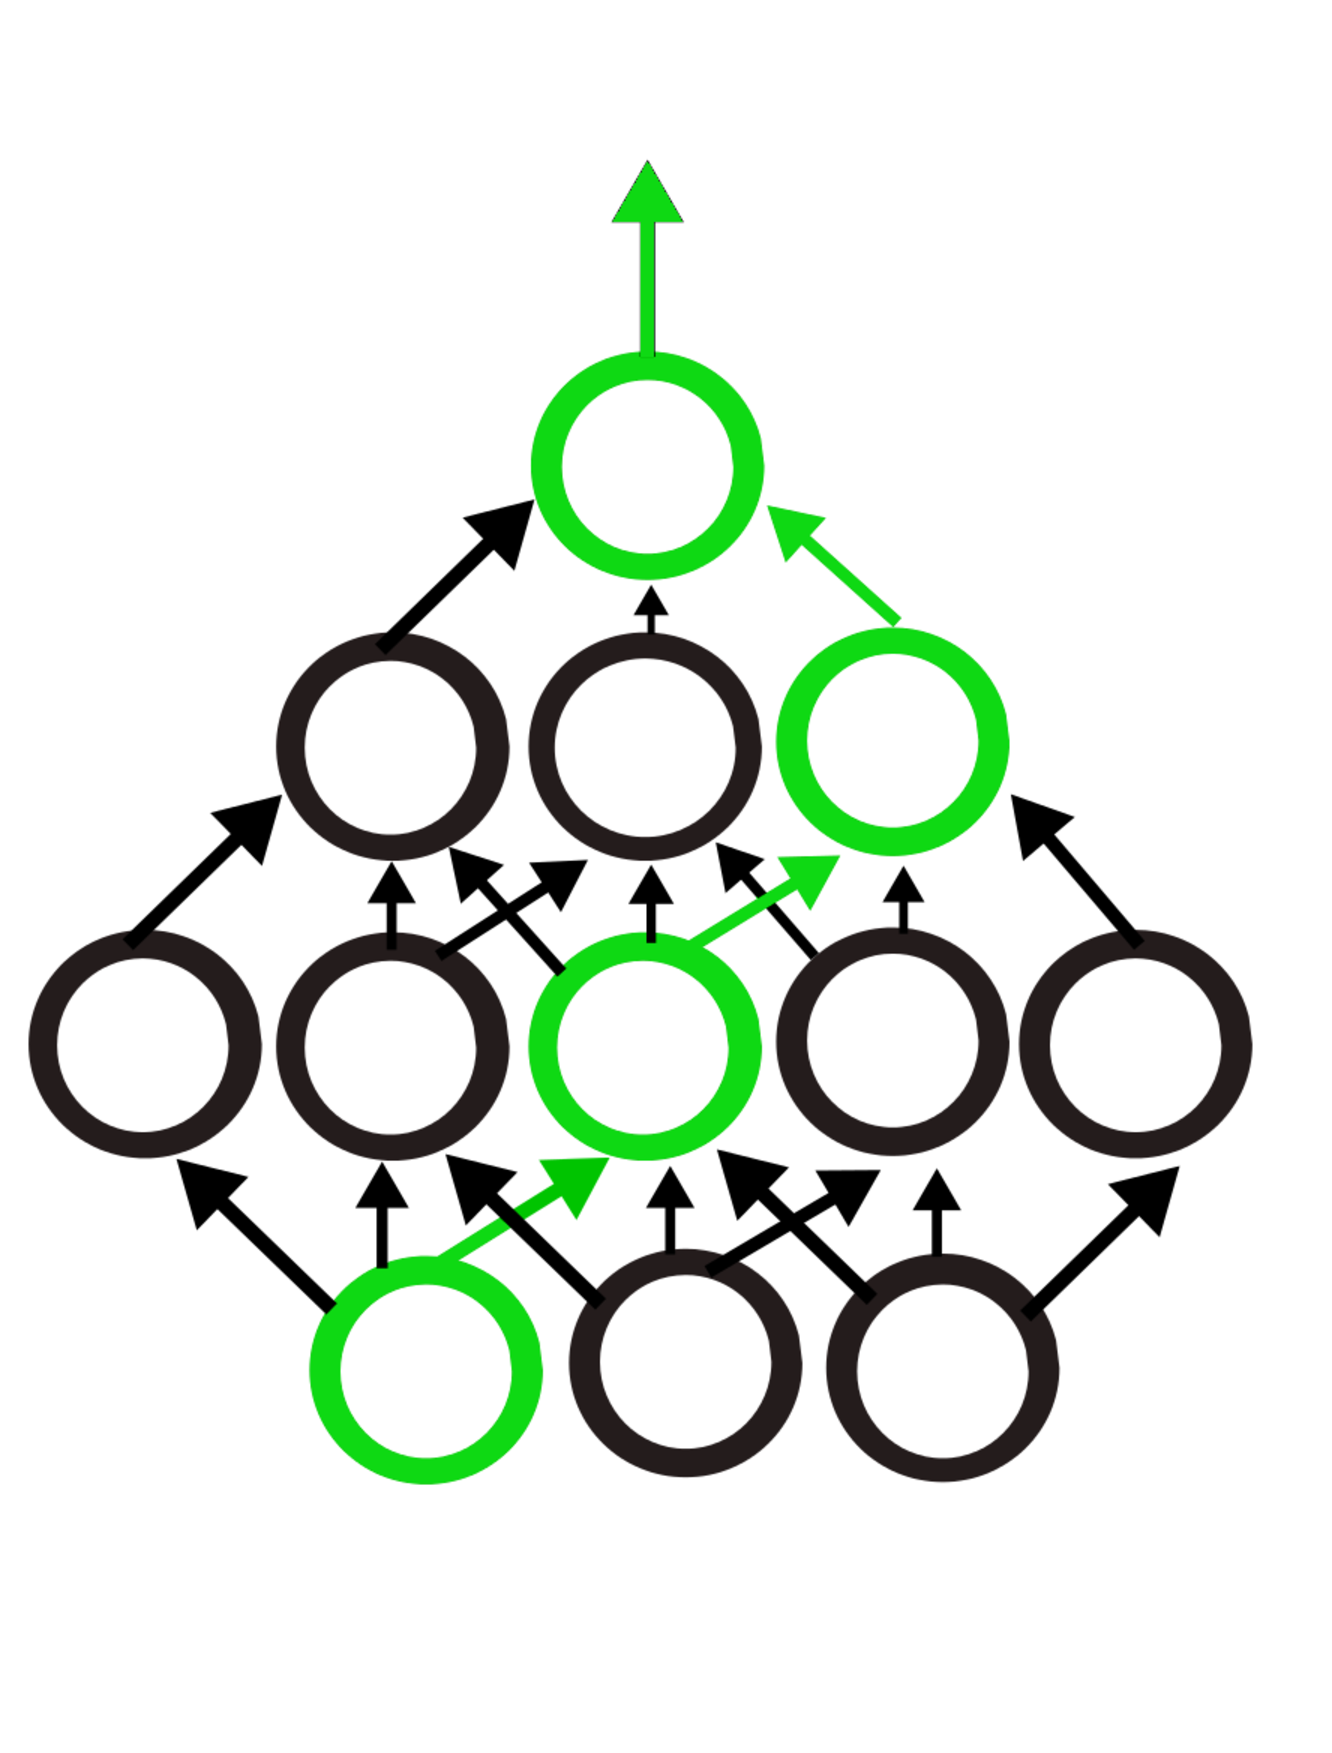
\includegraphics[width=0.5\textwidth]{figures/mlp_ticket_3.pdf}
	\end{figure}

\end{frame}

\begin{frame}{On the Transferability of Lottery Winners}

	\begin{figure}
		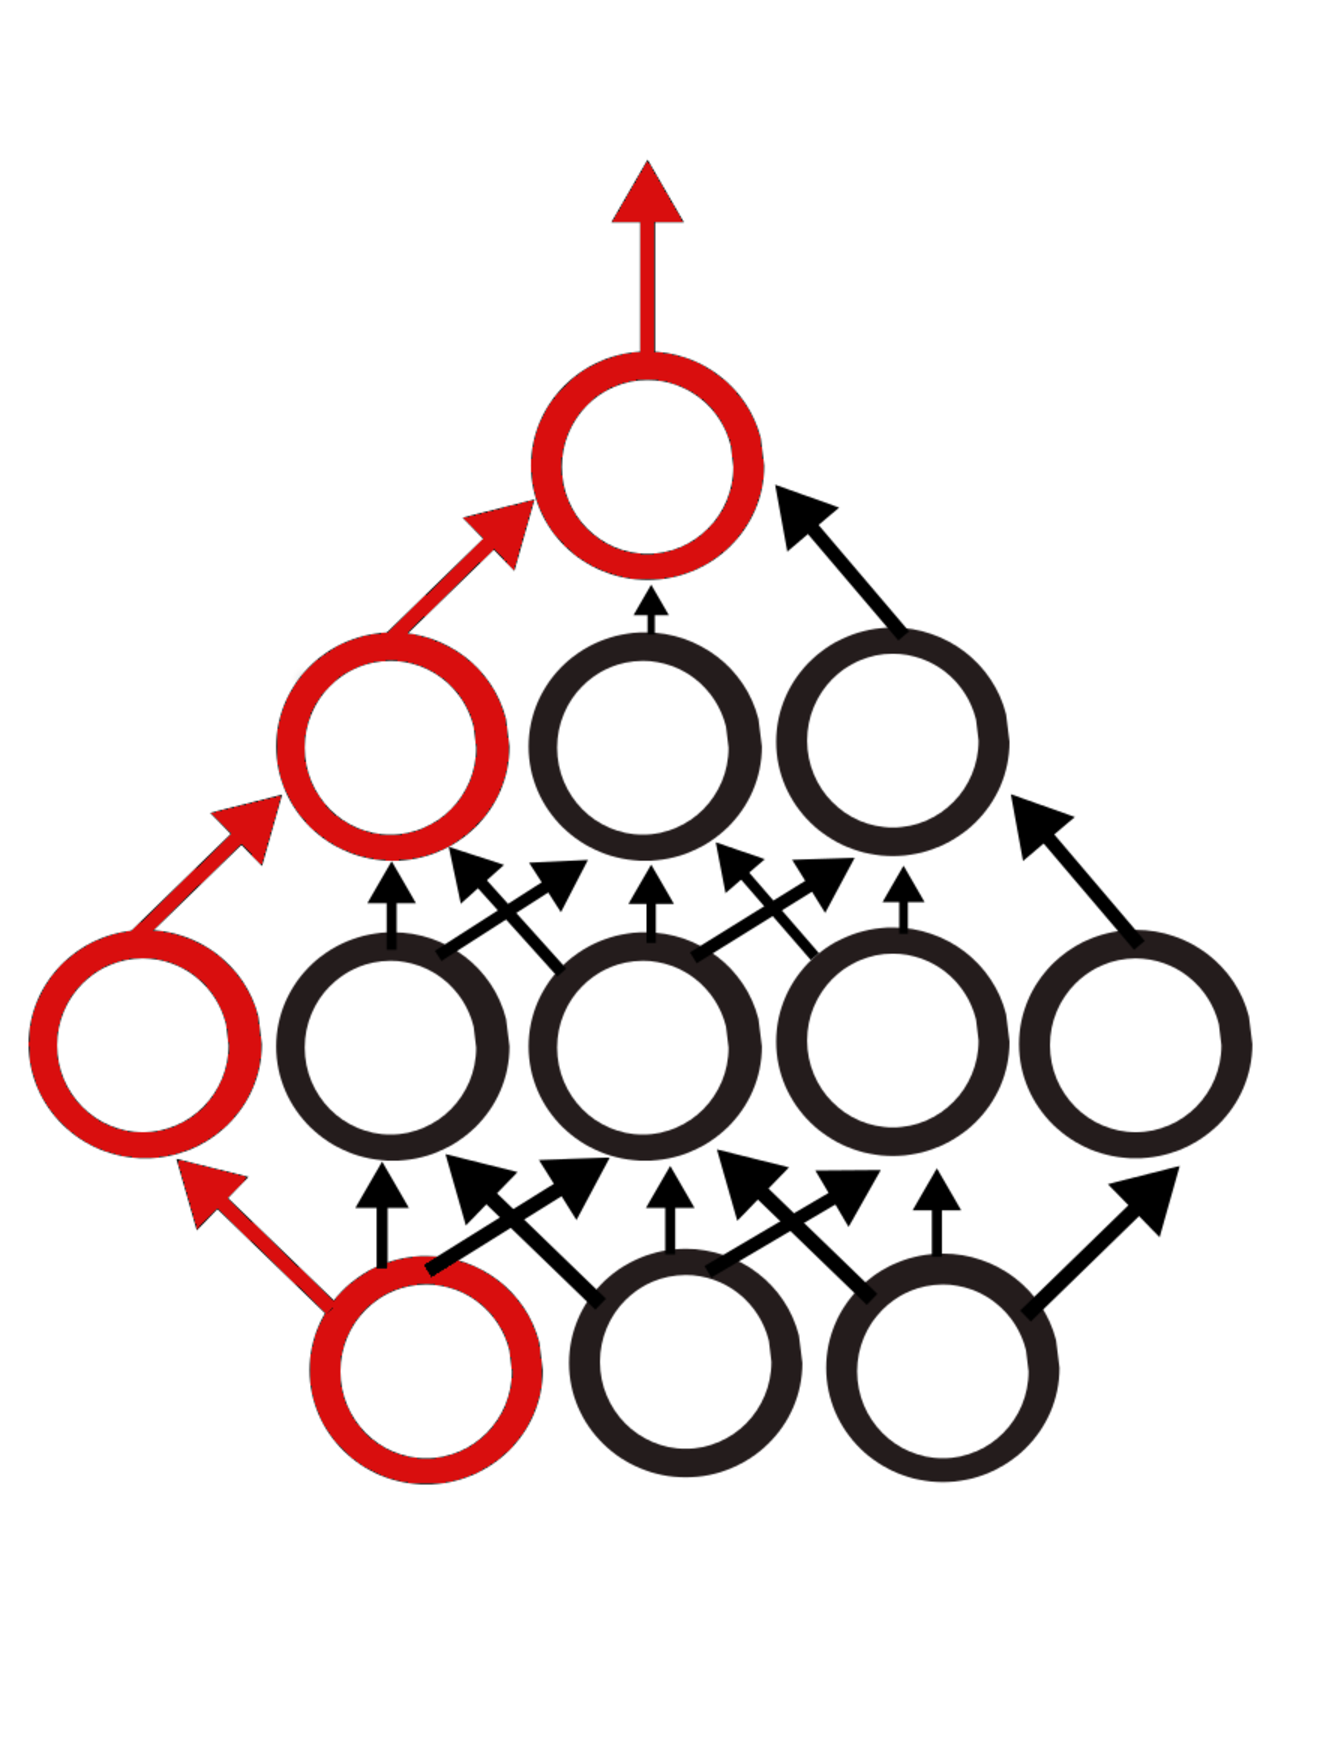
\includegraphics[width=0.5\textwidth]{figures/random_ticket_1.pdf}
	\end{figure}

\end{frame}

\begin{frame}{On the Transferability of Lottery Winners}

	\begin{figure}
		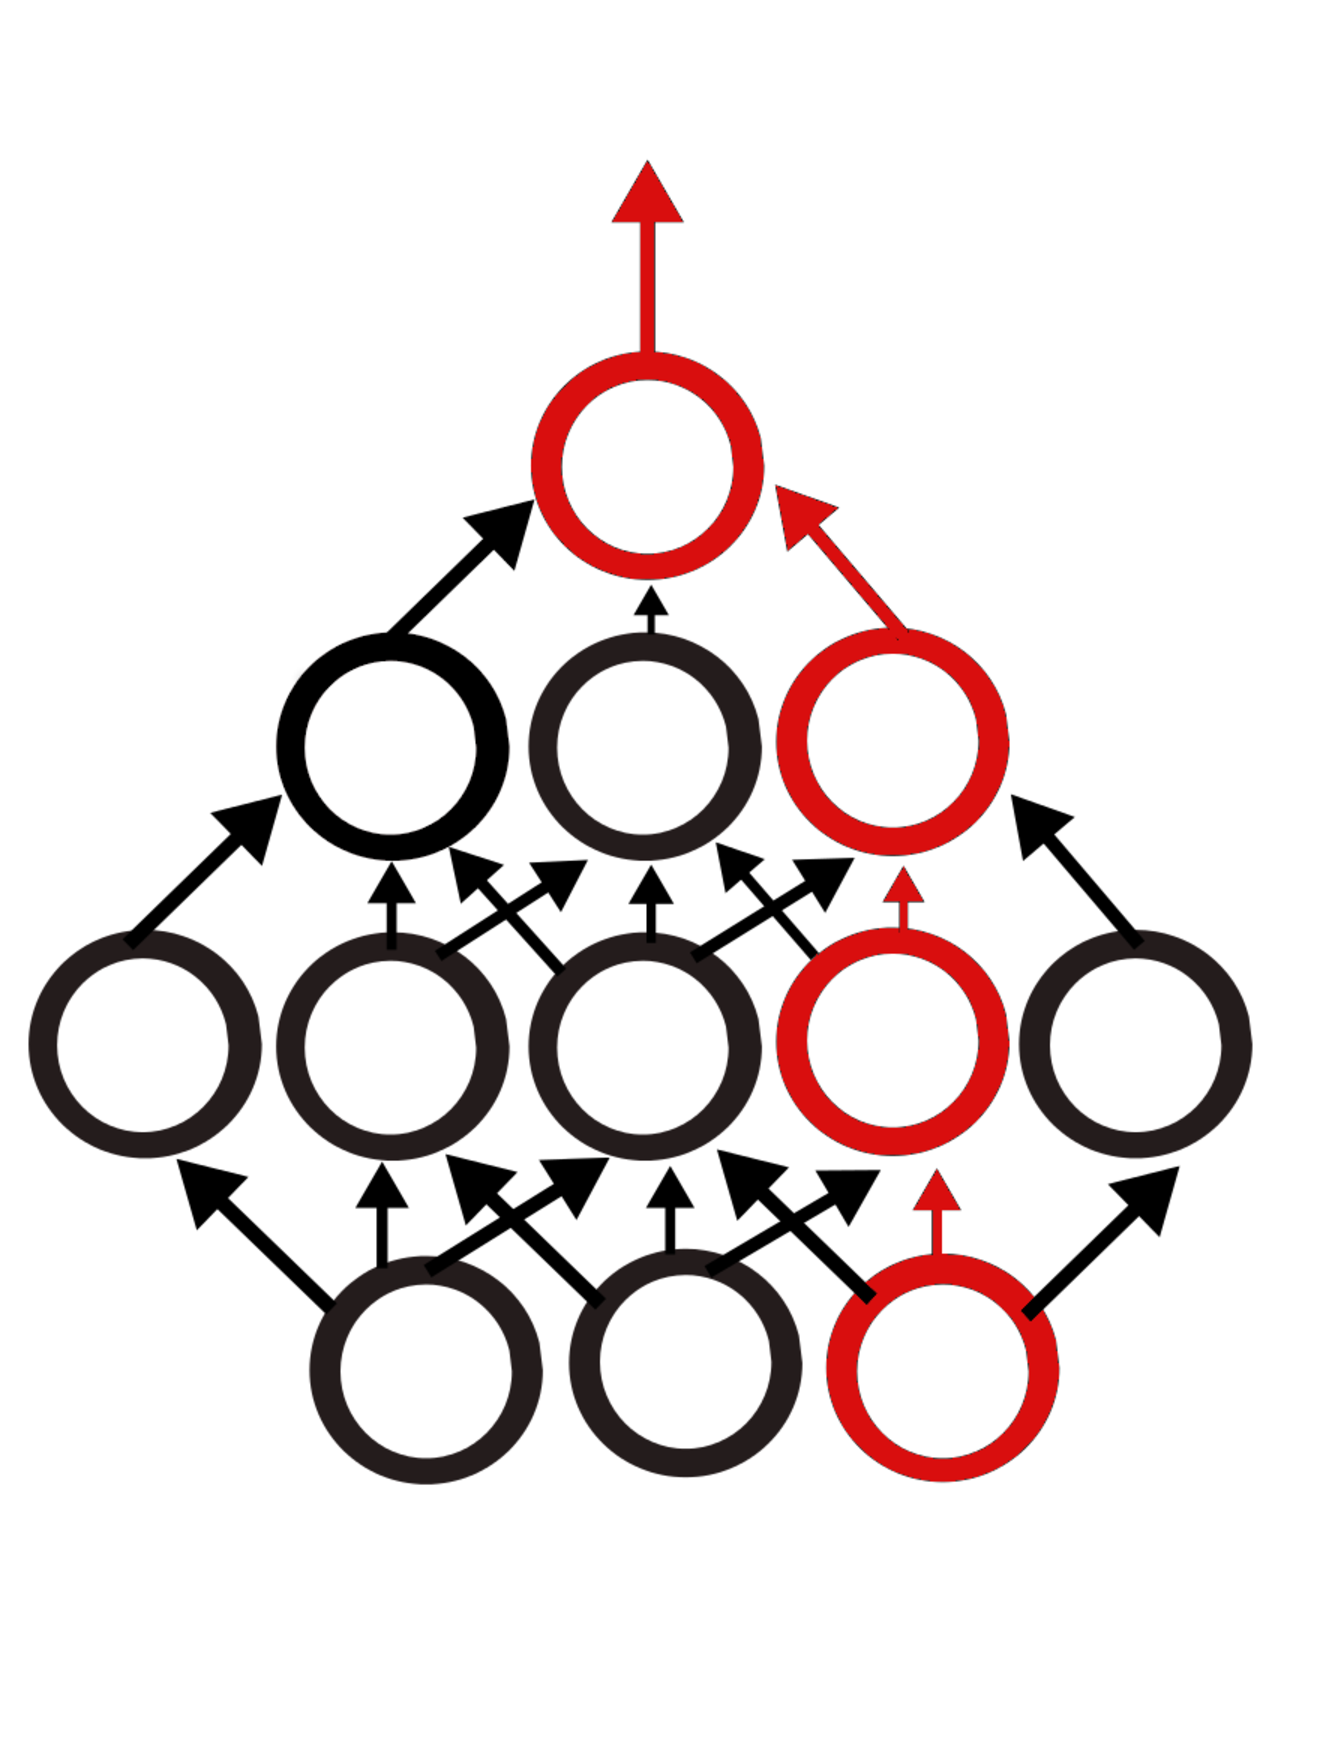
\includegraphics[width=0.5\textwidth]{figures/random_ticket_2.pdf}
	\end{figure}

\end{frame}


\begin{frame}{On the Transferability of Lottery Winners}

	$\Rightarrow$ How does one \textcolor{RoyalBlue}{find} a winning ticket?
	\bigskip
	
	\begin{itemize}
		\item Randomly initialize a network $f(x;\theta_0)$ where $\theta_0 \sim \mathscr{D}_{\theta}$
		\item We train the network for $j$ iterations
		\item We prune $p\%$ of the parameters in $\theta_j$ creating a mask $m$
		\item Reset the remaining parameters to their values at $\theta_0$, creating a winning ticket $f(x;m \odot \theta_0)$
	\end{itemize}

\end{frame}


\begin{frame}{On the Transferability of Lottery Winners}
	The Lottery Ticket Hypothesis in practice ...

	\begin{figure}[ht!]
  \centering
  \begin{tikzpicture}[scale = 0.45]
	\begin{axis}[
	grid style={dashed,gray},
	grid = both, 
	tick style=black,
	x label style={at={(axis description cs:0.5,-0.1)},anchor=north},
  	xlabel=Fraction of Weights Pruned,
  	ylabel= Accuracy ($\%$),
	title=CIFAR-10,
	%width=1,
	xtick=data,
	label style={font=\scriptsize},
	xticklabels = {0.0,0.2,0.36,0.488,0.59,0.672,0.738,0.79,0.832,0.866,0.893,0.914,0.931,0.945,0.956,0.965,0.972,0.977,0.982,0.986,0.988,0.991,0.993,0.994,0.995,0.996,0.997,0.998,0.998,0.998,0.999},
	x=4.5mm,
	ymin=0,
    	ymax=90,
	scale only axis,
	xticklabel style={rotate=90},
        %log ticks with fixed point,
        scaled ticks=true,
	/pgf/number format/fixed,
        %log ticks with fixed point,
  	legend pos=outer north east,
]

	\addlegendentry{Baseline}
	\addlegendentry{Winning Ticket $f(x;m\odot\theta_k)$}
	\addlegendentry{Random Mask + Random $\theta$}

\addplot [ultra thick, black, mark=x] table [x expr=\coordindex, y=baseline]{./Chapter06/logs/cifar10_example.txt};
%\addplot [ultra thick, blue, mark=x] table [x expr=\coordindex, y=ticket]{./Chapter06/logs/cifar10_example.txt};
%\addplot [ultra thick, red, mark=x] table [x expr=\coordindex, y=random_mask]{./Chapter06/logs/cifar10_example.txt};

\end{axis}
    \end{tikzpicture}

\end{figure} 

\end{frame}

\begin{frame}{On the Transferability of Lottery Winners}
	The Lottery Ticket Hypothesis in practice ...

	\begin{figure}[ht!]
  \centering
  \begin{tikzpicture}[scale = 0.45]
	\begin{axis}[
	grid style={dashed,gray},
	grid = both, 
	tick style=black,
	x label style={at={(axis description cs:0.5,-0.1)},anchor=north},
  	xlabel=Fraction of Weights Pruned,
  	ylabel= Accuracy ($\%$),
	title=CIFAR-10,
	%width=1,
	xtick=data,
	label style={font=\scriptsize},
	xticklabels = {0.0,0.2,0.36,0.488,0.59,0.672,0.738,0.79,0.832,0.866,0.893,0.914,0.931,0.945,0.956,0.965,0.972,0.977,0.982,0.986,0.988,0.991,0.993,0.994,0.995,0.996,0.997,0.998,0.998,0.998,0.999},
	x=4.5mm,
	ymin=0,
    	ymax=90,
	scale only axis,
	xticklabel style={rotate=90},
        %log ticks with fixed point,
        scaled ticks=true,
	/pgf/number format/fixed,
        %log ticks with fixed point,
  	legend pos=outer north east,
]

	\addlegendentry{Baseline}
	\addlegendentry{Winning Ticket $f(x;m\odot\theta_k)$}
	\addlegendentry{Random Mask + Random $\theta$}

\addplot [ultra thick, black, mark=x] table [x expr=\coordindex, y=baseline]{./Chapter06/logs/cifar10_example.txt};
\addplot [ultra thick, blue, mark=x] table [x expr=\coordindex, y=ticket]{./Chapter06/logs/cifar10_example.txt};
%\addplot [ultra thick, red, mark=x] table [x expr=\coordindex, y=random_mask]{./Chapter06/logs/cifar10_example.txt};

\end{axis}
    \end{tikzpicture}

\end{figure} 

\end{frame}



\begin{frame}{On the Transferability of Lottery Winners}
	The Lottery Ticket Hypothesis in practice ...

	\begin{figure}[ht!]
  \centering
  \begin{tikzpicture}[scale = 0.45]
	\begin{axis}[
	grid style={dashed,gray},
	grid = both, 
	tick style=black,
	x label style={at={(axis description cs:0.5,-0.1)},anchor=north},
  	xlabel=Fraction of Weights Pruned,
  	ylabel= Accuracy ($\%$),
	title=CIFAR-10,
	%width=1,
	xtick=data,
	label style={font=\scriptsize},
	xticklabels = {0.0,0.2,0.36,0.488,0.59,0.672,0.738,0.79,0.832,0.866,0.893,0.914,0.931,0.945,0.956,0.965,0.972,0.977,0.982,0.986,0.988,0.991,0.993,0.994,0.995,0.996,0.997,0.998,0.998,0.998,0.999},
	x=4.5mm,
	ymin=0,
    	ymax=90,
	scale only axis,
	xticklabel style={rotate=90},
        %log ticks with fixed point,
        scaled ticks=true,
	/pgf/number format/fixed,
        %log ticks with fixed point,
  	legend pos=outer north east,
]

	\addlegendentry{Baseline}
	\addlegendentry{Winning Ticket $f(x;m\odot\theta_k)$}
	\addlegendentry{Random Mask + Random $\theta$}

\addplot [ultra thick, black, mark=x] table [x expr=\coordindex, y=baseline]{./Chapter06/logs/cifar10_example.txt};
\addplot [ultra thick, blue, mark=x] table [x expr=\coordindex, y=ticket]{./Chapter06/logs/cifar10_example.txt};
\addplot [ultra thick, red, mark=x] table [x expr=\coordindex, y=random_mask]{./Chapter06/logs/cifar10_example.txt};

\end{axis}
    \end{tikzpicture}

\end{figure} 

\end{frame}

\begin{frame}{On the Transferability of Lottery Winners}
	Why are lottery tickets $f(x;m \odot \theta_0)$ so \textcolor{RoyalBlue}{special}?
	\begin{itemize}
		\item Train faster
		\item Faster Inference
		\item (Sometimes) obtain a better final performance
	\end{itemize}
	\bigskip
	However ... 

	\begin{itemize}
		\item Identifying a winning ticket is \textcolor{Maroon}{computationally expensive} 
		\item We \textcolor{Maroon}{do not} know how and why lottery winners appear throughout learning
	\end{itemize}
\end{frame}

\begin{frame}{On the Transferability of Lottery Winners}

	$\Rightarrow$ Therefore we study whether winning tickets $f(x;m \odot \theta_0)$
	found on natural image datasets can get \textcolor{RoyalBlue}{transferred} to the non-natural realm

	\bigskip

	We use three popular Computer Vision datasets as source domains $\mathcal{D}_S$:

	\begin{figure}
 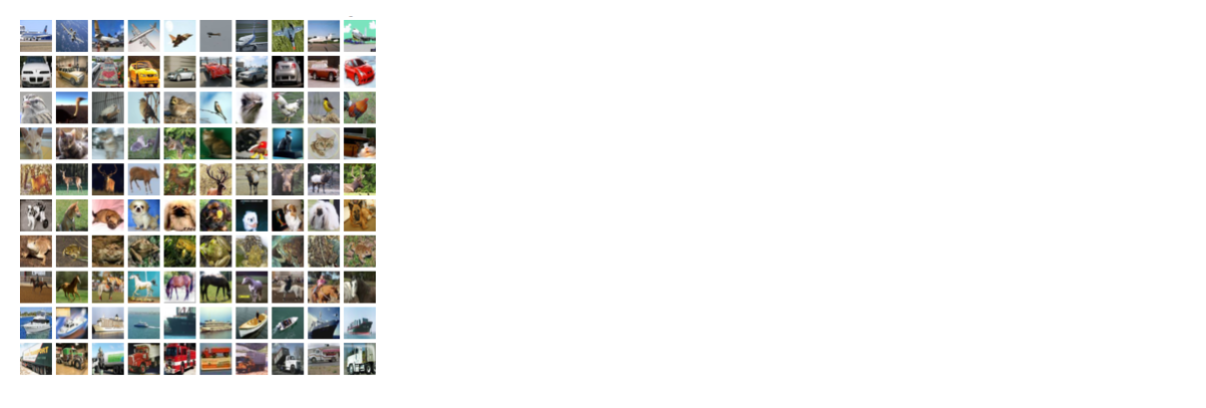
\includegraphics[width=0.8\textwidth]{figures/cifar10}
\end{figure}
\end{frame}

\begin{frame}{On the Transferability of Lottery Winners}

	$\Rightarrow$ Therefore we study whether winning tickets $f(x;m \odot \theta_0)$
	found on natural image datasets can get \textcolor{RoyalBlue}{transferred} to the non-natural realm

	\bigskip

	We use three popular Computer Vision datasets as source domains $\mathcal{D}_S$:

	\begin{figure}
 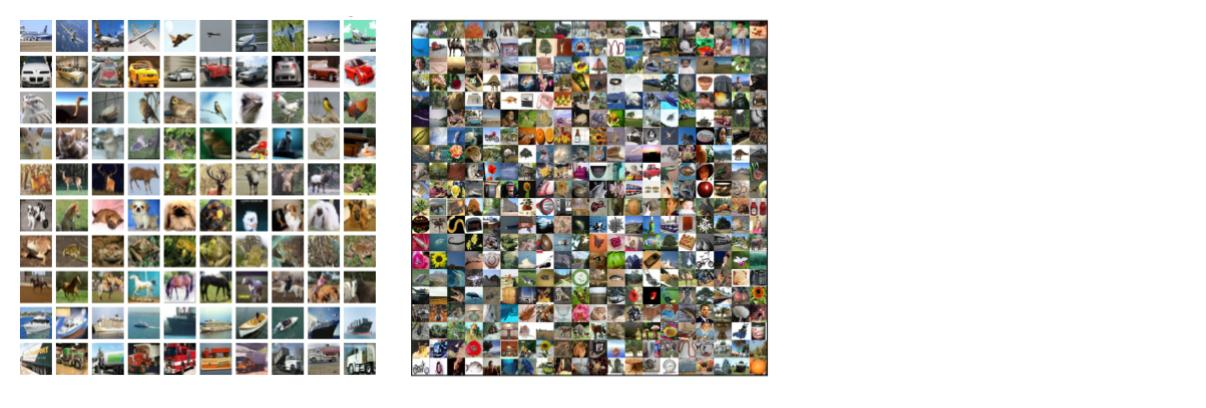
\includegraphics[width=0.8\textwidth]{figures/cifar100}
\end{figure}
\end{frame}

\begin{frame}{On the Transferability of Lottery Winners}

	$\Rightarrow$ Therefore we study whether winning tickets $f(x;m \odot \theta_0)$
	found on natural image datasets can get \textcolor{RoyalBlue}{transferred} to the non-natural realm

	\bigskip

	We use three popular Computer Vision datasets as source domains $\mathcal{D}_S$

	\begin{figure}
 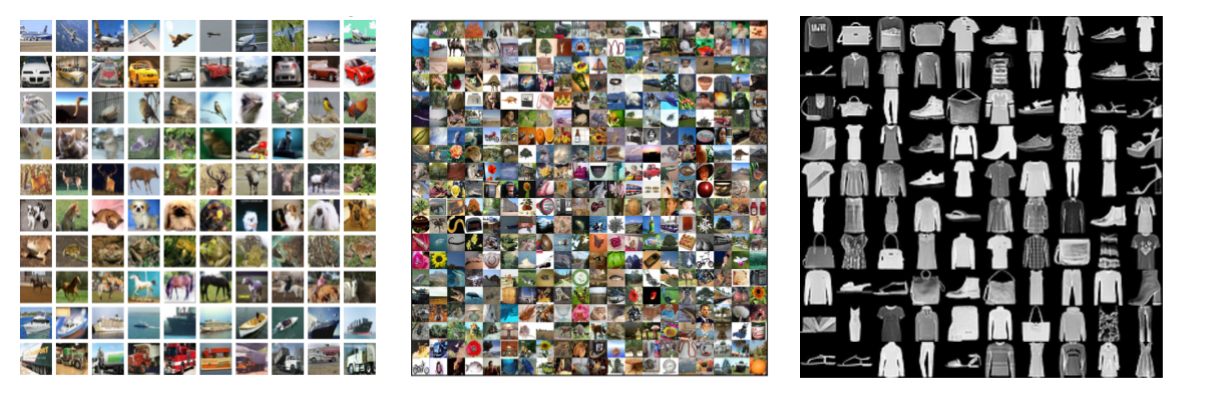
\includegraphics[width=0.8\textwidth]{figures/fashion_mnist}
\end{figure}
\end{frame}


\begin{frame}{On the Transferability of Lottery Winners}

	And we use \textcolor{RoyalBlue}{seven datasets} of non-natural images as target tasks $\mathcal{T}_T$ coming from the fields of Digital Pathology and Digital Heritage

	\begin{figure}
 		\centering
  		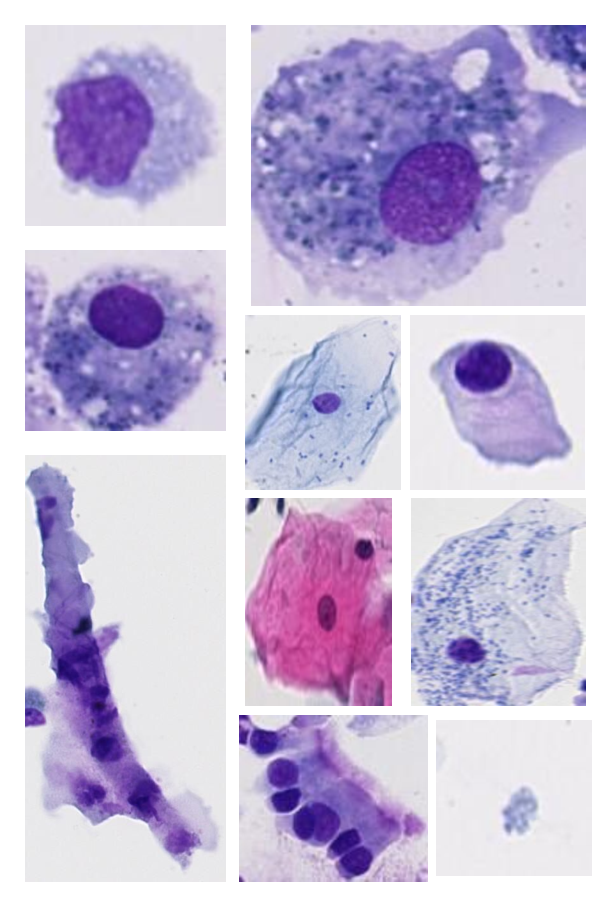
\includegraphics[width=1.8cm,height=\textheight,keepaspectratio]{figures/lba.pdf}%
  		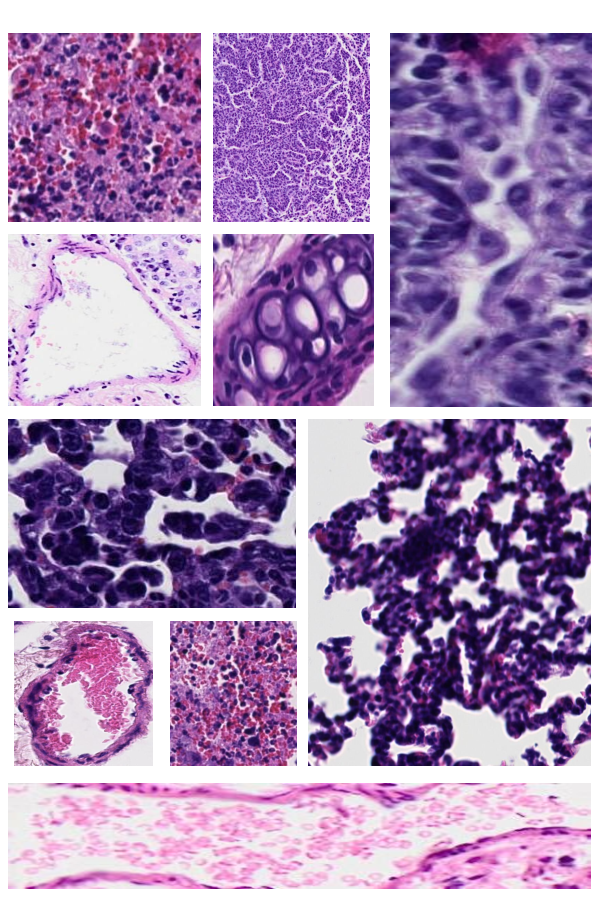
\includegraphics[width=1.8cm,height=\textheight,keepaspectratio]{figures/tissus.pdf}%
  		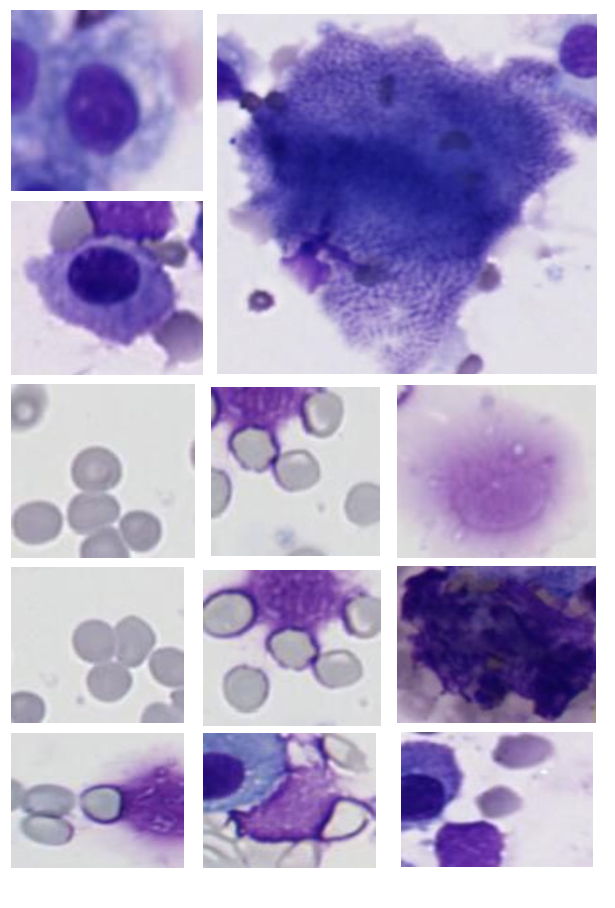
\includegraphics[width=1.8cm,height=\textheight,keepaspectratio]{figures/mouse_lba.pdf}%
  		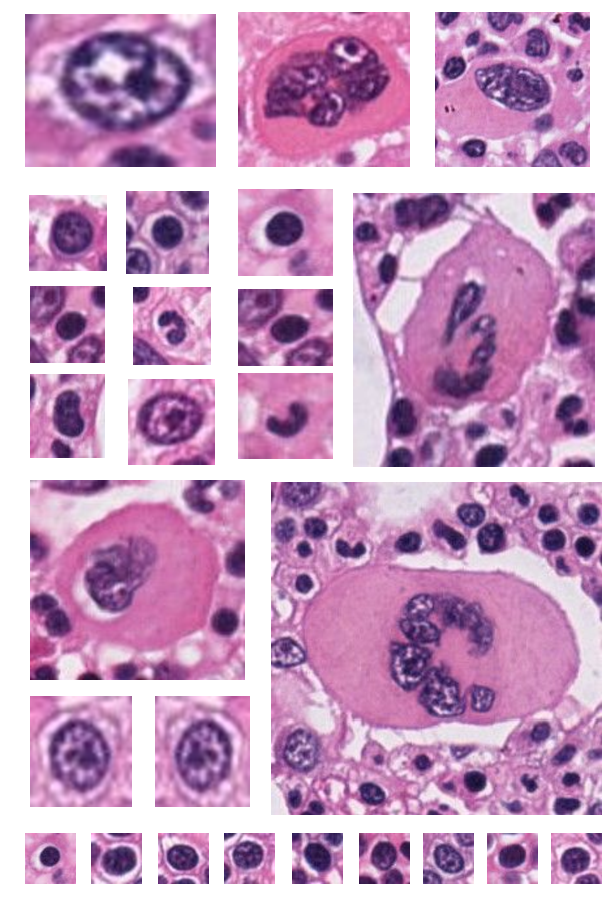
\includegraphics[width=1.8cm,height=\textheight,keepaspectratio]{figures/bonemarrow.pdf}%
    		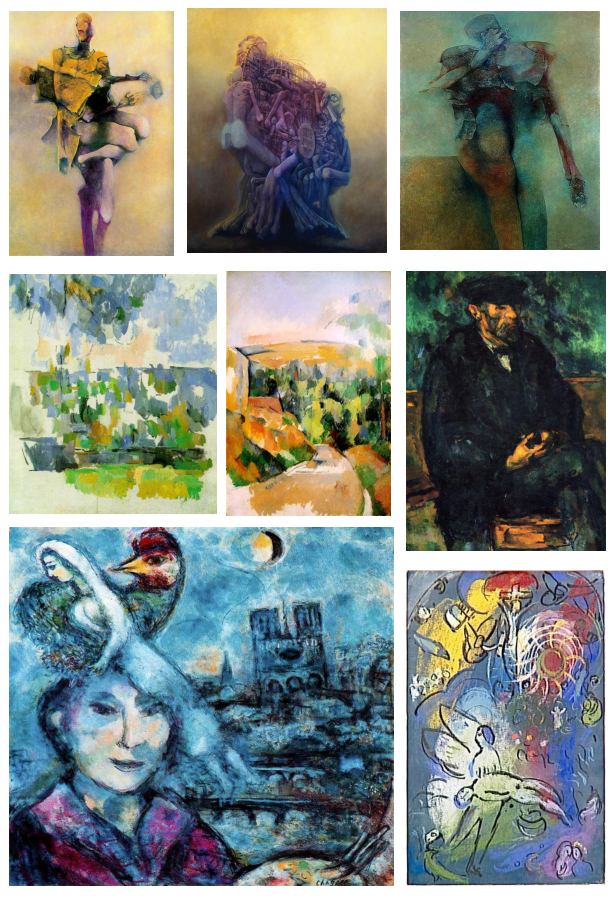
\includegraphics[width=1.8cm,height=\textheight,keepaspectratio]{figures/artist.pdf}%
  		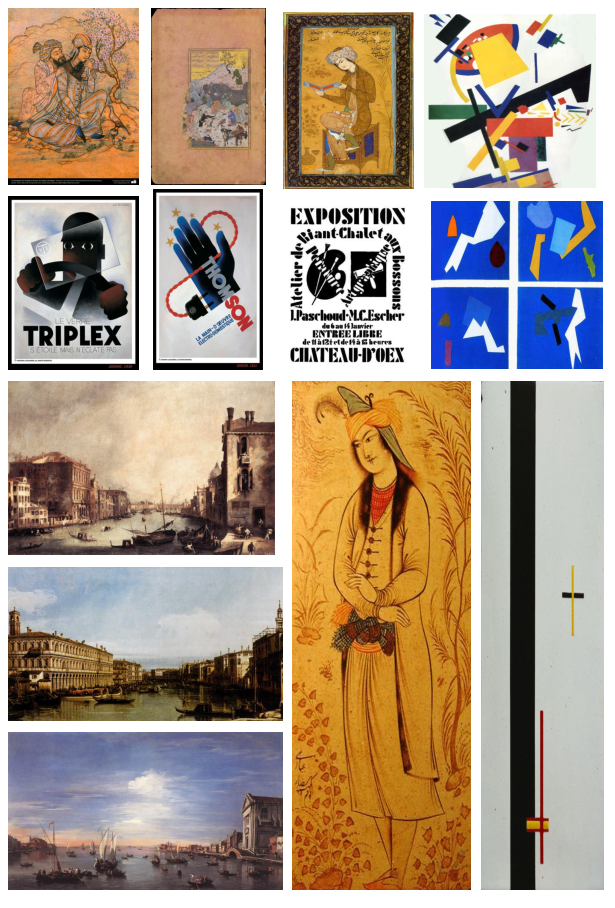
\includegraphics[width=1.8cm,height=\textheight,keepaspectratio]{figures/type.pdf}%
	\end{figure}

\end{frame}


\begin{frame}{On the Transferability of Lottery Winners}
	Transferring lottery winners to the \textcolor{RoyalBlue}{Digital Pathology} data ...
	\begin{figure}[ht!]
\centering
	\begin{tikzpicture}[scale = 0.5]

\begin{axis}[
	name=ax1,
	grid style={dashed,gray},
	grid = both, 
	tick style=black,
  	x label style={at={(axis description cs:0.5,-0.1)},anchor=north},
	xlabel=Fraction of Weights Pruned,
  	ylabel= Accuracy ($\%$),
	ylabel style={font=\Large},
	title=Human-LBA,
	xtick=data,
	legend pos=south west,
	label style={font=\scriptsize},
	xticklabels = {0.0,0.2,0.36,0.488,0.59,0.672,0.738,0.79,0.832,0.866,0.893,0.914,0.931,0.945,0.956,0.965,0.972,0.977,0.982,0.986,0.988,0.991,0.993,0.994,0.995,0.996,0.997,0.998,0.998,0.998,0.999},
	x=4.5mm,
	ymin=40,
    	ymax=90,
	scale only axis,
	xticklabel style={rotate=90},
        %log ticks with fixed point,
        scaled ticks=true,
	/pgf/number format/fixed,
        %log ticks with fixed point,
]

	\addlegendentry{Baseline}
	\addlegendentry{Winning Ticket $f(x;m\odot\theta_k)$}
	\addlegendentry{Random Ticket $f(x;m\odot\theta_r)$}
	\addlegendentry{CIFAR-10}
	\addlegendentry{CIFAR-100}
	\addlegendentry{Fashion-MNIST}


\addplot [ultra thick, black, mark=x] table [x expr=\coordindex, y=baseline]{./Chapter06/logs/human_lba.txt};
%\addplot [ultra thick, blue, mark=x] table [x expr=\coordindex, y=winning_ticket]{./Chapter06/logs/human_lba.txt};
%\addplot [ultra thick, orange, mark=x] table [x expr=\coordindex, y=random_mask]{./Chapter06/logs/human_lba.txt};
%\addplot [ultra thick, green, mark=x] table [x expr=\coordindex, y=cifar10]{./Chapter06/logs/human_lba.txt};
%\addplot [ultra thick, red, mark=x] table [x expr=\coordindex, y=cifar100]{./Chapter06/logs/human_lba.txt};
%\addplot [ultra thick, purple, mark=x] table [x expr=\coordindex, y=fahion_mnist]{./Chapter06/logs/human_lba.txt};

\end{axis}
\end{tikzpicture}
\end{figure} 


\end{frame}

\begin{frame}{On the Transferability of Lottery Winners}
	Transferring lottery winners to the \textcolor{RoyalBlue}{Digital Pathology} data ...
	\begin{figure}[ht!]
\centering
	\begin{tikzpicture}[scale = 0.5]

\begin{axis}[
	name=ax1,
	grid style={dashed,gray},
	grid = both, 
	tick style=black,
  	x label style={at={(axis description cs:0.5,-0.1)},anchor=north},
	xlabel=Fraction of Weights Pruned,
  	ylabel= Accuracy ($\%$),
	ylabel style={font=\Large},
	title=Human-LBA,
	xtick=data,
	legend pos=south west,
	label style={font=\scriptsize},
	xticklabels = {0.0,0.2,0.36,0.488,0.59,0.672,0.738,0.79,0.832,0.866,0.893,0.914,0.931,0.945,0.956,0.965,0.972,0.977,0.982,0.986,0.988,0.991,0.993,0.994,0.995,0.996,0.997,0.998,0.998,0.998,0.999},
	x=4.5mm,
	ymin=40,
    	ymax=90,
	scale only axis,
	xticklabel style={rotate=90},
        %log ticks with fixed point,
        scaled ticks=true,
	/pgf/number format/fixed,
        %log ticks with fixed point,
]

	\addlegendentry{Baseline}
	\addlegendentry{Winning Ticket $f(x;m\odot\theta_k)$}
	\addlegendentry{Random Ticket $f(x;m\odot\theta_r)$}
	\addlegendentry{CIFAR-10}
	\addlegendentry{CIFAR-100}
	\addlegendentry{Fashion-MNIST}


\addplot [ultra thick, black, mark=x] table [x expr=\coordindex, y=baseline]{./Chapter06/logs/human_lba.txt};
\addplot [ultra thick, blue, mark=x] table [x expr=\coordindex, y=winning_ticket]{./Chapter06/logs/human_lba.txt};
%\addplot [ultra thick, orange, mark=x] table [x expr=\coordindex, y=random_mask]{./Chapter06/logs/human_lba.txt};
%\addplot [ultra thick, green, mark=x] table [x expr=\coordindex, y=cifar10]{./Chapter06/logs/human_lba.txt};
%\addplot [ultra thick, red, mark=x] table [x expr=\coordindex, y=cifar100]{./Chapter06/logs/human_lba.txt};
%\addplot [ultra thick, purple, mark=x] table [x expr=\coordindex, y=fahion_mnist]{./Chapter06/logs/human_lba.txt};

\end{axis}
\end{tikzpicture}
\end{figure} 

\end{frame}


\begin{frame}{On the Transferability of Lottery Winners}
		Transferring lottery winners to the \textcolor{RoyalBlue}{Digital Pathology} data ...
\begin{figure}[ht!]
\centering
	\begin{tikzpicture}[scale = 0.5]

\begin{axis}[
	name=ax1,
	grid style={dashed,gray},
	grid = both, 
	tick style=black,
  	x label style={at={(axis description cs:0.5,-0.1)},anchor=north},
	xlabel=Fraction of Weights Pruned,
  	ylabel= Accuracy ($\%$),
	ylabel style={font=\Large},
	title=Human-LBA,
	xtick=data,
	legend pos=south west,
	label style={font=\scriptsize},
	xticklabels = {0.0,0.2,0.36,0.488,0.59,0.672,0.738,0.79,0.832,0.866,0.893,0.914,0.931,0.945,0.956,0.965,0.972,0.977,0.982,0.986,0.988,0.991,0.993,0.994,0.995,0.996,0.997,0.998,0.998,0.998,0.999},
	x=4.5mm,
	ymin=40,
    	ymax=90,
	scale only axis,
	xticklabel style={rotate=90},
        %log ticks with fixed point,
        scaled ticks=true,
	/pgf/number format/fixed,
        %log ticks with fixed point,
]

	\addlegendentry{Baseline}
	\addlegendentry{Winning Ticket $f(x;m\odot\theta_k)$}
	\addlegendentry{Random Ticket $f(x;m\odot\theta_r)$}
	\addlegendentry{CIFAR-10}
	\addlegendentry{CIFAR-100}
	\addlegendentry{Fashion-MNIST}


\addplot [ultra thick, black, mark=x] table [x expr=\coordindex, y=baseline]{./Chapter06/logs/human_lba.txt};
\addplot [ultra thick, blue, mark=x] table [x expr=\coordindex, y=winning_ticket]{./Chapter06/logs/human_lba.txt};
\addplot [ultra thick, orange, mark=x] table [x expr=\coordindex, y=random_mask]{./Chapter06/logs/human_lba.txt};
%\addplot [ultra thick, green, mark=x] table [x expr=\coordindex, y=cifar10]{./Chapter06/logs/human_lba.txt};
%\addplot [ultra thick, red, mark=x] table [x expr=\coordindex, y=cifar100]{./Chapter06/logs/human_lba.txt};
%\addplot [ultra thick, purple, mark=x] table [x expr=\coordindex, y=fahion_mnist]{./Chapter06/logs/human_lba.txt};

\end{axis}
\end{tikzpicture}
\end{figure} 

\end{frame}


\begin{frame}{On the Transferability of Lottery Winners}
		Transferring lottery winners to the \textcolor{RoyalBlue}{Digital Pathology} data ...
\begin{figure}[ht!]
\centering
	\begin{tikzpicture}[scale = 0.5]

\begin{axis}[
	name=ax1,
	grid style={dashed,gray},
	grid = both, 
	tick style=black,
  	x label style={at={(axis description cs:0.5,-0.1)},anchor=north},
	xlabel=Fraction of Weights Pruned,
  	ylabel= Accuracy ($\%$),
	ylabel style={font=\Large},
	title=Human-LBA,
	xtick=data,
	legend pos=south west,
	label style={font=\scriptsize},
	xticklabels = {0.0,0.2,0.36,0.488,0.59,0.672,0.738,0.79,0.832,0.866,0.893,0.914,0.931,0.945,0.956,0.965,0.972,0.977,0.982,0.986,0.988,0.991,0.993,0.994,0.995,0.996,0.997,0.998,0.998,0.998,0.999},
	x=4.5mm,
	ymin=40,
    	ymax=90,
	scale only axis,
	xticklabel style={rotate=90},
        %log ticks with fixed point,
        scaled ticks=true,
	/pgf/number format/fixed,
        %log ticks with fixed point,
]

	\addlegendentry{Baseline}
	\addlegendentry{Winning Ticket $f(x;m\odot\theta_k)$}
	\addlegendentry{Random Ticket $f(x;m\odot\theta_r)$}
	\addlegendentry{CIFAR-10}
	\addlegendentry{CIFAR-100}
	\addlegendentry{Fashion-MNIST}


\addplot [ultra thick, black, mark=x] table [x expr=\coordindex, y=baseline]{./Chapter06/logs/human_lba.txt};
\addplot [ultra thick, blue, mark=x] table [x expr=\coordindex, y=winning_ticket]{./Chapter06/logs/human_lba.txt};
\addplot [ultra thick, orange, mark=x] table [x expr=\coordindex, y=random_mask]{./Chapter06/logs/human_lba.txt};
\addplot [ultra thick, green, mark=x] table [x expr=\coordindex, y=cifar10]{./Chapter06/logs/human_lba.txt};
%\addplot [ultra thick, red, mark=x] table [x expr=\coordindex, y=cifar100]{./Chapter06/logs/human_lba.txt};
%\addplot [ultra thick, purple, mark=x] table [x expr=\coordindex, y=fahion_mnist]{./Chapter06/logs/human_lba.txt};

\end{axis}
\end{tikzpicture}
\end{figure} 

\end{frame}


\begin{frame}{On the Transferability of Lottery Winners}
		Transferring lottery winners to the \textcolor{RoyalBlue}{Digital Pathology} data ...
\begin{figure}[ht!]
\centering
	\begin{tikzpicture}[scale = 0.5]

\begin{axis}[
	name=ax1,
	grid style={dashed,gray},
	grid = both, 
	tick style=black,
  	x label style={at={(axis description cs:0.5,-0.1)},anchor=north},
	xlabel=Fraction of Weights Pruned,
  	ylabel= Accuracy ($\%$),
	ylabel style={font=\Large},
	title=Human-LBA,
	xtick=data,
	legend pos=south west,
	label style={font=\scriptsize},
	xticklabels = {0.0,0.2,0.36,0.488,0.59,0.672,0.738,0.79,0.832,0.866,0.893,0.914,0.931,0.945,0.956,0.965,0.972,0.977,0.982,0.986,0.988,0.991,0.993,0.994,0.995,0.996,0.997,0.998,0.998,0.998,0.999},
	x=4.5mm,
	ymin=40,
    	ymax=90,
	scale only axis,
	xticklabel style={rotate=90},
        %log ticks with fixed point,
        scaled ticks=true,
	/pgf/number format/fixed,
        %log ticks with fixed point,
]

	\addlegendentry{Baseline}
	\addlegendentry{Winning Ticket $f(x;m\odot\theta_k)$}
	\addlegendentry{Random Ticket $f(x;m\odot\theta_r)$}
	\addlegendentry{CIFAR-10}
	\addlegendentry{CIFAR-100}
	\addlegendentry{Fashion-MNIST}


\addplot [ultra thick, black, mark=x] table [x expr=\coordindex, y=baseline]{./Chapter06/logs/human_lba.txt};
\addplot [ultra thick, blue, mark=x] table [x expr=\coordindex, y=winning_ticket]{./Chapter06/logs/human_lba.txt};
\addplot [ultra thick, orange, mark=x] table [x expr=\coordindex, y=random_mask]{./Chapter06/logs/human_lba.txt};
\addplot [ultra thick, green, mark=x] table [x expr=\coordindex, y=cifar10]{./Chapter06/logs/human_lba.txt};
\addplot [ultra thick, red, mark=x] table [x expr=\coordindex, y=cifar100]{./Chapter06/logs/human_lba.txt};
%\addplot [ultra thick, purple, mark=x] table [x expr=\coordindex, y=fahion_mnist]{./Chapter06/logs/human_lba.txt};

\end{axis}
\end{tikzpicture}
\end{figure} 

\end{frame}

\begin{frame}{On the Transferability of Lottery Winners}
	Transferring lottery winners to the \textcolor{RoyalBlue}{Digital Pathology} data ...
	\begin{figure}[ht!]
\centering
	\begin{tikzpicture}[scale = 0.5]

\begin{axis}[
	name=ax1,
	grid style={dashed,gray},
	grid = both, 
	tick style=black,
  	x label style={at={(axis description cs:0.5,-0.1)},anchor=north},
	xlabel=Fraction of Weights Pruned,
  	ylabel= Accuracy ($\%$),
	ylabel style={font=\Large},
	title=Human-LBA,
	xtick=data,
	legend pos=south west,
	label style={font=\scriptsize},
	xticklabels = {0.0,0.2,0.36,0.488,0.59,0.672,0.738,0.79,0.832,0.866,0.893,0.914,0.931,0.945,0.956,0.965,0.972,0.977,0.982,0.986,0.988,0.991,0.993,0.994,0.995,0.996,0.997,0.998,0.998,0.998,0.999},
	x=4.5mm,
	ymin=40,
    	ymax=90,
	scale only axis,
	xticklabel style={rotate=90},
        %log ticks with fixed point,
        scaled ticks=true,
	/pgf/number format/fixed,
        %log ticks with fixed point,
]

	\addlegendentry{Baseline}
	\addlegendentry{Winning Ticket $f(x;m\odot\theta_k)$}
	\addlegendentry{Random Ticket $f(x;m\odot\theta_r)$}
	\addlegendentry{CIFAR-10}
	\addlegendentry{CIFAR-100}
	\addlegendentry{Fashion-MNIST}


\addplot [ultra thick, black, mark=x] table [x expr=\coordindex, y=baseline]{./Chapter06/logs/human_lba.txt};
\addplot [ultra thick, blue, mark=x] table [x expr=\coordindex, y=winning_ticket]{./Chapter06/logs/human_lba.txt};
\addplot [ultra thick, orange, mark=x] table [x expr=\coordindex, y=random_mask]{./Chapter06/logs/human_lba.txt};
\addplot [ultra thick, green, mark=x] table [x expr=\coordindex, y=cifar10]{./Chapter06/logs/human_lba.txt};
\addplot [ultra thick, red, mark=x] table [x expr=\coordindex, y=cifar100]{./Chapter06/logs/human_lba.txt};
\addplot [ultra thick, purple, mark=x] table [x expr=\coordindex, y=fahion_mnist]{./Chapter06/logs/human_lba.txt};

\end{axis}
\end{tikzpicture}
\end{figure} 

\end{frame}

\begin{frame}{On the Transferability of Lottery Winners}
	Transferring lottery winners to the \textcolor{RoyalBlue}{Digital Heritage} data ...
	\begin{figure}[ht!]
\centering
	\begin{tikzpicture}[scale = 0.5]
\begin{axis}[
	name=ax1,
	grid style={dashed,gray},
	grid = both, 
	tick style=black,
	x label style={at={(axis description cs:0.5,-0.1)},anchor=north},
  	xlabel=Fraction of Weights Pruned,
  	ylabel= Accuracy ($\%$),
	title=Artist Classification 1,
	%width=1,
	xtick=data,
	legend pos=south west,
	label style={font=\scriptsize},
	xticklabels = {0.0,0.2,0.36,0.488,0.59,0.672,0.738,0.79,0.832,0.866,0.893,0.914,0.931,0.945,0.956,0.965,0.972,0.977,0.982,0.986,0.988,0.991,0.993,0.994,0.995,0.996,0.997,0.998,0.998,0.998,0.999},
	x=4.5mm,
	ymin=0,
    	ymax=75,
	scale only axis,
	xticklabel style={rotate=90},
        %log ticks with fixed point,
        scaled ticks=true,
	/pgf/number format/fixed,
        %log ticks with fixed point,
  	%legend pos=outer north east,
	%legend style={font=\small, at={(-0.8,-0.2,-0.2)},anchor=north west, legend columns = 1}
	]

	\addlegendentry{Baseline}
	\addlegendentry{Winning Ticket $f(x;m\odot\theta_k)$}
	\addlegendentry{Random Ticket $f(x;m\odot\theta_r)$}
	\addlegendentry{CIFAR-10}
	\addlegendentry{CIFAR-100}
	\addlegendentry{Fashion-MNIST}


\addplot [ultra thick, black, mark=x] table [x expr=\coordindex, y=baseline]{./Chapter06/logs/artist_classification_1.txt};
\addplot [ultra thick, blue, mark=x] table [x expr=\coordindex, y=winning_ticket]{./Chapter06/logs/artist_classification_1.txt};
\addplot [ultra thick, orange, mark=x] table [x expr=\coordindex, y=random_mask]{./Chapter06/logs/artist_classification_1.txt};
\addplot [ultra thick, green, mark=x] table [x expr=\coordindex, y=cifar10]{./Chapter06/logs/artist_classification_1.txt};
\addplot [ultra thick, red, mark=x] table [x expr=\coordindex, y=cifar100]{./Chapter06/logs/artist_classification_1.txt};
\addplot [ultra thick, purple, mark=x] table [x expr=\coordindex, y=fahion_mnist]{./Chapter06/logs/artist_classification_1.txt};

\end{axis}    
\end{tikzpicture}
\end{figure} 

\end{frame}



\begin{frame}{On the Transferability of Lottery Winners}

	Our main findings show that on Digital Pathology data
	\bigskip
	\begin{itemize}
		\item All lottery winners \textcolor{RoyalBlue}{significantly outperfom} unpruned models 
		\item Natural lottery winners contain \textcolor{RoyalBlue}{a generic inductive bias} (to some extent)
		\item Best performance is obtained by identifying a winning ticket directly on the \textcolor{Maroon}{target task} $\mathcal{T}_T$
	\end{itemize}
	\bigskip

	whereas on Digital Heritage data
	\bigskip
	\begin{itemize}
		\item Natural lottery winners transfer \textcolor{RoyalBlue}{much better}
		\item They can even \textcolor{RoyalBlue}{outperform} target task $\mathcal{T}_T$ tickets
	\end{itemize}
\end{frame}

\begin{frame}{On the Transferability of Lottery Winners}
	
	We also provide additional empirical insights into the Lottery Ticket Hypothesis:
	\bigskip
	\begin{itemize}
		\item We show that completely pre-trained winning tickets $f(x;m \odot \theta_i)$ \textcolor{Maroon}{overfit} on the source task $\mathcal{T}_S$ 
		\item The presence of winning tickets \textcolor{Maroon}{does not depend} on the size of the training data
		\item The closer the source task $\mathcal{S}_T$ and the target task $\mathcal{T}_T$ the \textcolor{RoyalBlue}{better} the transferability of $f(x;m \odot \theta_k)$
	\end{itemize}

\end{frame}

%============================================================================

\begin{frame}
	\begin{center}
		\textcolor{skymagenta}{\textbf{PART III}}
	\end{center}
\end{frame}


%============================================================================


\begin{frame}{A Novel Family of DRL Algorithms}
	\section{Part III: Reinforcement Learning}
	\subsection{A Novel Family of DRL Algorithms}
\end{frame}

\begin{frame}{A Novel Family of DRL Algorithms}

	\bigskip
	We now consider a different machine learning paradigm: \textcolor{RoyalBlue}{Reinforcement Learning} (RL), where an agent needs to learn how to interact with its environment

	\begin{figure}[htb!]
		\centering
		\tikzset{
  frame/.style={
    rectangle, draw,
    text width=6em, text centered,
    minimum height=4em,drop shadow,fill=white,
    rounded corners,
  },
  line/.style={
    draw, -{Latex},rounded corners=3mm,
  }
}

\begin{tikzpicture}[font=\small\sffamily\bfseries,very thick,node distance = 4cm]
\node [frame] (agent) {Agent};
\node [frame, below=1.2cm of agent] (environment) {Environment};
\draw[line] (agent.0) -- ++ (1.5,0) |- (environment.0) 
node[right,pos=0.25,align=left] {action\\ $a_t$};
\coordinate[left=8mm of environment] (P);
\draw[thin,dashed] (P|-environment.north) -- (P|-environment.south);
\draw[line] (environment.200) -- (P |- environment.200)
node[midway,above]{$s_{t+1}$};
\draw[line,thick] (environment.160) -- (P |- environment.160)
node[midway,above]{$r_{t+1}$};
\draw[line] (P |- environment.200) -- ++ (-1.4,0) |- (agent.160)
node[left, pos=0.25, align=right] {state\\ $s_t$};
\draw[line,thick] (P |- environment.160) -- ++ (-0.8,0) |- (agent.200)
node[right,pos=0.25,align=left] {reward\\ $r_t$};
\end{tikzpicture}


 		\label{fig:rl_loop}
	\end{figure}

\end{frame}

\begin{frame}{A Novel Family of DRL Algorithms}
	Such interaction is modeled as a \textcolor{RoyalBlue}{Markov Decision Process} (MDP) consisting of the following elements:

\begin{itemize}
	\item A set of possible states $\mathcal{S}$,
	\item A set of possible actions $\mathcal{A}$,
	\item A transition function $\mathcal{P}:\mathcal{S}\times\mathcal{A}\times\mathcal{S}\rightarrow [0,1]$,
	\item A reward function $\Re:\mathcal{S}\times\mathcal{A}\times\mathcal{S}\rightarrow \mathbb{R}$,
	\item A discount factor denoted as $\gamma \in [0,1]$.
\end{itemize}

\bigskip

Therefore we can define an MDP as $\mathcal{M}=\langle\mathcal{S}, \mathcal{A}, \mathcal{P}, \Re, \gamma\rangle$.

\end{frame}

\begin{frame}{A Novel Family of DRL Algorithms}	
	\bigskip

	The interaction between the agent and the environment is given by the agent's \textcolor{RoyalBlue}{policy} $\pi$, a probability distribution over $a \in \mathcal{A}(s)$ for each $s \in \mathcal{S}$:

	\begin{equation*}
	\pi(a|s) = \text{Pr}\; \{a_t = a | s_t = s\}, \; \text{for all}\; s \in \mathcal{S}\; \text{and}\; a\ \in \mathcal{A}.
	\end{equation*}

	\bigskip

	The \textcolor{RoyalBlue}{goal} of the agent is to maximize the expected discounted return as:
	\begin{equation*}
		\begin{split}
			G_t & = r_t+\gamma r_{t+1} + \gamma^{2} r_{t+2} + ... \\
	    			& = \sum_{k=0}^{\infty}\gamma^{k} r_{t+k}.
		\end{split}
		\label{eq:discounted_return}
	\end{equation*}

\end{frame}


\begin{frame}{A Novel Family of DRL Algorithms}	
	\bigskip
	In RL some components of the MDP are unknown 
	\begin{center}
		$\mathcal{M}=\langle\mathcal{S}, \mathcal{A}, \textcolor{red}{\mathcal{P}}, \textcolor{red}{\Re}, \gamma\rangle$,
	\end{center}
	
	which in the case of \textcolor{RoyalBlue}{model-free} RL can be overcome by learning either the state-value function

	\begin{align*}
    		V^{\pi}(s)=\mathds{E}\bigg[\sum_{k=0}^{\infty}\gamma^{k}r_{t+k}\bigg| s_t = s, \pi \bigg],
	\end{align*}

	or the state-action value function

	\begin{align*}
     		Q^{\pi}(s,a)=\mathds{E}\bigg[\sum_{k=0}^{\infty}\gamma^{k}r_{t+k} \bigg| s_t = s, a_t=a, \pi\bigg].
	\end{align*}
\end{frame}


\begin{frame}{A Novel Family of DRL Algorithms}
	\begin{itemize}
		\item Model-free algorithms are implemented in a \textcolor{RoyalBlue}{tabular} fashion, meaning that the state values, or state-action values, are stored within tables of sizes $|\mathcal{S}|$ and $|\mathcal{S}\times\mathcal{A}|$ respectively

		\item For many problems we typically seek to learn an \textcolor{RoyalBlue}{approximation} of the value functions
	\end{itemize}
	
	\begin{center}

		$V^{\pi}(s)\approx V^\pi{(s;\theta)}$ and $Q^{\pi}(s,a;\theta)\approx Q(s,a;\theta)$
	\end{center}
	
	\bigskip

	This approximation can be represented by a \textcolor{RoyalBlue}{Convolutional Neural Network}

\end{frame}

\begin{frame}{A Novel Family of DRL Algorithms}
	Typical DRL algorithms aim at only learning an approximation of the state-action value function $Q^{\pi}(s,a)\approx Q^{\pi}(s,a;\theta)$

	\begin{itemize}
		\item A policy $\pi$ can only be derived from $Q^{\pi}(s,a)$ 
		\item It is hard to combine RL algorithms with neural networks
		\item Dealing with one value function can be complicated enough
	\end{itemize}

	\bigskip

	However ...

	\begin{itemize}
		\item Training can be very slow 
		\item Algorithms are prone to diverge
		\item Do not correctly estimate $Q^{\pi}(s,a)$
	\end{itemize}

\end{frame}

\begin{frame}{A Novel Family of DRL Algorithms}	
	\bigskip

	$\Rightarrow$ Therefore we suggest to \textcolor{RoyalBlue}{jointly approximate} the state-value function $V^{\pi}(s;\phi)$ alongside the state-action value function $Q^{\pi}(s,a;\theta)$

	\bigskip

	We can do this by either training a \textcolor{skymagenta}{\textbf{DQV}} agent which learns $V^{\pi}(s;\phi)$ by minimizing
		\begin{multline*}
L(\phi) = \mathds{E}_{\langle s_{t},a_{t},r_{t},s_{t+1}\rangle\sim U(D)} \bigg[\big(r_{t} + \gamma V(s_{t+1}; \phi^{-}) - V(s_{t}; \phi)\big)^{2}\bigg],
		\end{multline*}			
		and $Q^{\pi}(s,a)$ with:
		\begin{multline*}
    			L(\theta) = \mathds{E}_{\langle s_{t},a_{t},r_{t},s_{t+1}\rangle\sim U(D)} \bigg[\big(r_{t} + \gamma V(s_{t+1}; \phi^{-}) - Q(s_{t}, a_{t}; \theta)\big)^{2}\bigg],
		\end{multline*}

\end{frame}

\begin{frame}{A Novel Family of DRL Algorithms}
	... or by training a \textcolor{skymagenta}{\textbf{DQV-Max}} agent that learns $V^{\pi}(s;\phi)$ with
	\begin{multline*}
		L(\phi) = \mathds{E}_{\langle s_{t},a_{t},r_{t},s_{t+1}\rangle\sim U(D)} \bigg[\big(r_{t} + \gamma \: \underset{a\in \mathcal{A}}{\max}\: Q(s_{t+1}, a; \theta^{-}) - V(s_{t}; \phi)\big)^{2}\bigg],
	\end{multline*}
	and $Q^{\pi}(s,a)$ with:
	\begin{multline*}
    		L(\theta) = \mathds{E}_{\langle s_{t},a_{t},r_{t},s_{t+1}\rangle\sim U(D)} \bigg[\big(r_{t} + \gamma V(s_{t+1}; \phi) - Q(s_{t}, a_{t}; \theta)\big)^{2}\bigg].
	\end{multline*}
\end{frame}

\begin{frame}{A Novel Family of DRL Algorithms}
	\bigskip

	$\Rightarrow$ We compare their performance to algorithms which only learn an approximation of the state-action value function $Q^\pi(s,a)$ \footnote{Mnih, Volodymyr, et al. "Human-level control through deep reinforcement learning." nature 518.7540 (2015)} \footnote{Van Hasselt, Hado, Arthur Guez, and David Silver. "Deep reinforcement learning with double q-learning." Proceedings of the AAAI conference on artificial intelligence (2016).}

\end{frame}

\begin{frame}{A Novel Family of DRL Algorithms}
	\begin{figure}[ht!]
  \begin{tikzpicture}[scale = 0.4]
      \begin{axis}[
	name=ax1,
      	grid style={dashed,gray},
      	grid = both, 
      	tick style=black,
	title=Boxing,
        xlabel=Episodes,
        ylabel=Reward,
      ]


      %\addlegendentry{DQV} 
      %\addlegendentry{DQV-Max}  
      \addlegendentry{DQN}
      \addlegendentry{DDQN}
      
      %\addplot [ultra thick, red, mark=.] table [y=DQV, x=episodes]
      %{./Chapter07/logs/boxing_results.txt};
      % \addplot [ultra thick, yellow, mark=.] table [y=DQV-Max, x=episodes]
      %{./Chapter07/logs/boxing_results.txt};
      \addplot [ultra thick, blue, mark=.] table [y=DQN, x=episodes]{./Chapter07/logs/boxing_results.txt};
      \addplot [ultra thick, green, mark=.] table [y=DDQN, x=episodes]{./Chapter07/logs/boxing_results.txt};
     
      \legend{}

      \end{axis}

      \begin{axis}[
      	at={(ax1.south east)},
	xshift=2cm,
	grid style={dashed,gray},
      	grid = both, 
      	tick style=black,
	title=Enduro,
        xlabel=Episodes,
        ylabel=Reward,
      ]


      %\addlegendentry{DQV} 
      %\addlegendentry{DQV-Max}  
      \addlegendentry{DQN}
      \addlegendentry{DDQN}
      
      %\addplot [ultra thick, red, mark=.] table [y=DQV, x=episodes]
      %{./Chapter07/logs/enduro_results.txt};
       %\addplot [ultra thick, yellow, mark=.] table [y=DQV-Max, x=episodes]
      %{./Chapter07/logs/enduro_results.txt};
      \addplot [ultra thick, blue, mark=.] table [y=DQN, x=episodes]{./Chapter07/logs/enduro_results.txt};
      \addplot [ultra thick, green, mark=.] table [y=DDQN, x=episodes]{./Chapter07/logs/enduro_results.txt};
     
      \legend{}

      \end{axis}


      \begin{axis}[
	at={(ax1.south east)},
	xshift=-2cm,
      	yshift=-8cm,
	grid style={dashed,gray},
      	grid = both, 
      	tick style=black,
	title=Pong,
        xlabel=Episodes,
        ylabel= Reward,
	legend columns=4, 
        legend style={font=\Large, at={(0.15,-0.3,-0.4)},anchor=north west,legend columns=3},
      ]


	%\addlegendentry{DQV} 
	%\addlegendentry{DQV-Max}  
	\addlegendentry{DQN}
	\addlegendentry{DDQN}

      %\addplot [ultra thick, red, mark=.] table [y=DQV, x=episodes]
      %{./Chapter07/logs/pong_results.txt};
      %\addplot [ultra thick, yellow, mark=.] table [y=DQV-Max, x=episodes]
      %{./Chapter07/logs/pong_results.txt};
      
      \addplot [ultra thick, blue, mark=.] table [y=DQN, x=episodes]{./Chapter07/logs/pong_results.txt};
      \addplot [ultra thick, green, mark=.] table [y=DDQN, x=episodes]{./Chapter07/logs/pong_results.txt};
 
      \end{axis}
	\end{tikzpicture}
\end{figure}


\end{frame}

\begin{frame}{A Novel Family of DRL Algorithms}
	\begin{figure}[ht!]
  \begin{tikzpicture}[scale = 0.4]
      \begin{axis}[
	name=ax1,
      	grid style={dashed,gray},
      	grid = both, 
      	tick style=black,
	title=Boxing,
        xlabel=Episodes,
        ylabel=Reward,
      ]


      \addlegendentry{DQV} 
      \addlegendentry{DQV-Max}  
      \addlegendentry{DQN}
      \addlegendentry{DDQN}
      
      \addplot [ultra thick, red, mark=.] table [y=DQV, x=episodes]
      {./Chapter07/logs/boxing_results.txt};
       \addplot [ultra thick, yellow, mark=.] table [y=DQV-Max, x=episodes]
      {./Chapter07/logs/boxing_results.txt};
      \addplot [ultra thick, blue, mark=.] table [y=DQN, x=episodes]{./Chapter07/logs/boxing_results.txt};
      \addplot [ultra thick, green, mark=.] table [y=DDQN, x=episodes]{./Chapter07/logs/boxing_results.txt};
     
      \legend{}

      \end{axis}

      \begin{axis}[
      	at={(ax1.south east)},
	xshift=2cm,
	grid style={dashed,gray},
      	grid = both, 
      	tick style=black,
	title=Enduro,
        xlabel=Episodes,
        ylabel=Reward,
      ]


      \addlegendentry{DQV} 
      \addlegendentry{DQV-Max}  
      \addlegendentry{DQN}
      \addlegendentry{DDQN}
      
      \addplot [ultra thick, red, mark=.] table [y=DQV, x=episodes]
      {./Chapter07/logs/enduro_results.txt};
      \addplot [ultra thick, yellow, mark=.] table [y=DQV-Max, x=episodes]
      {./Chapter07/logs/enduro_results.txt};
      \addplot [ultra thick, blue, mark=.] table [y=DQN, x=episodes]{./Chapter07/logs/enduro_results.txt};
      \addplot [ultra thick, green, mark=.] table [y=DDQN, x=episodes]{./Chapter07/logs/enduro_results.txt};
     
      \legend{}

      \end{axis}


      \begin{axis}[
	at={(ax1.south east)},
	xshift=-2cm,
      	yshift=-8cm,
	grid style={dashed,gray},
      	grid = both, 
      	tick style=black,
	title=Pong,
        xlabel=Episodes,
        ylabel= Reward,
	legend columns=4, 
        legend style={font=\Large, at={(-0.15,-0.3,-0.4)},anchor=north west,legend columns=3},
      ]


	\addlegendentry{DQV} 
	\addlegendentry{DQV-Max}  
	\addlegendentry{DQN}
	\addlegendentry{DDQN}

      \addplot [ultra thick, red, mark=.] table [y=DQV, x=episodes]
      {./Chapter07/logs/pong_results.txt};
      \addplot [ultra thick, yellow, mark=.] table [y=DQV-Max, x=episodes]
      {./Chapter07/logs/pong_results.txt};
      
      \addplot [ultra thick, blue, mark=.] table [y=DQN, x=episodes]{./Chapter07/logs/pong_results.txt};
      \addplot [ultra thick, green, mark=.] table [y=DDQN, x=episodes]{./Chapter07/logs/pong_results.txt};
 
      \end{axis}
	\end{tikzpicture}
\end{figure}


\end{frame}

\begin{frame}{A Novel Family of DRL Algorithms}
	$\Rightarrow$ Jointly approximating two value functions over one results in \textcolor{RoyalBlue}{faster convergence}, but also in \textcolor{RoyalBlue}{accurate} value estimates:

	\begin{figure}[ht!]
  \begin{tikzpicture}[scale = 0.55]
      \begin{axis}[
	name=ax1,
      	grid style={dashed,gray},
      	grid = both, 
      	tick style=black,
	title=Pong,
        xlabel=Training Steps,
        ylabel=Value Estimates,
      ]


      \addlegendentry{DQN-True Value}
      \addlegendentry{DQN-Estimated Value}
      
      \addplot [ultra thick, black, mark=.] table [y=true_return_DQN, x=training_steps]
      {./Chapter07/logs/overestimation_pong.txt};
      \addplot [ultra thick, blue, mark=.] table [y=estimate_DQN, x=training_steps]{./Chapter07/logs/overestimation_pong.txt};
     
      \end{axis}

      \begin{axis}[
	at={(ax1.south east)},
	xshift=2cm,
      	grid style={dashed,gray},
      	grid = both, 
      	tick style=black,
	title=Pong,
        xlabel=Training Steps,
        ylabel= Value Estimates,
	%legend columns=3, 
        %legend style={font=\Large, at={(-1,-0.3,-0.4)},anchor=north west,legend columns=3},
      ]

      \addlegendentry{DQV-Max-True Value}
      \addlegendentry{DQV-Max-Estimated Value}

      \addplot [ultra thick, black, mark=.] table [y=true_return_DQV-Max, x=training_steps]
      {./Chapter07/logs/overestimation_pong.txt};
      \addplot [ultra thick, yellow, mark=.] table [y=estimate_DQV-Max, x=training_steps]{./Chapter07/logs/overestimation_pong.txt};
 
      \end{axis}
	\end{tikzpicture}
\end{figure}



\end{frame}

\begin{frame}{A Novel Family of DRL Algorithms}
	To conclude DQV-Learning and DQV-Max Learning

	\begin{itemize}
		\item Result in \textcolor{RoyalBlue}{faster learning}
		\item Are \textcolor{RoyalBlue}{robust} to the "Deadly Triad of DRL"
		\item Suffer \textcolor{RoyalBlue}{less} from the overestimation bias of the $Q$ function 
		\item \textcolor{RoyalBlue}{Scale well} to the multi-agent setting \footnote{Leroy, Pascal, et al. "QVMix and QVMix-Max: Extending the Deep Quality-Value Family of Algorithms to Cooperative Multi-Agent Reinforcement Learning." (2021).}
	\end{itemize}

	However ... 

	\begin{itemize}
		\item Memory wise are \textcolor{Maroon}{twice} as expensive as DQN and DDQN
		\item \textcolor{Maroon}{Do not} always result in better policies
	\end{itemize}

\end{frame}


\begin{frame}{On the Transferability of Deep-Q Networks}
	\subsection{On the Transferability of Deep-Q Networks}

\end{frame}

\begin{frame}{On the Transferability of Deep-Q Networks}
	
	Let's take a look at the performance of the DQV algorithms more closely ...
	
	\bigskip
	\begin{table*}[ht]
\caption{The results obtained by DQV and DQV-Max on a subset of 15 \texttt{Atari} games, compared with those obtained by DQN and DDQN (reproduced from their corresponding publications). We can see that our newly introduced algorithms have a comparable, and often even better performance than DQN and DDQN. As highlighted by the green cells the overall best performing algorithm in our set of experiments is DQV-Max while the second-best performing algorithm is DQV (as reported by the yellow cells). Specific attention should be given to the games \texttt{BankHeist} and \texttt{Enduro} where DQV and DQV-Max are the only algorithms which can master the game with a final super-human performance.}
\centering
\resizebox{\columnwidth}{!}{%
\begin{tabular}{l|r|r|r|r|r|r}
\hline 
Environment & Random & Human & DQN \cite{mnih2015human} & DDQN \cite{van2016deep} & DQV & DQV-Max\\
\hline \hline
\texttt{Asteroids} &719.10 &13156.70 &\cellcolor{yellow!25}1629.33 &930.60 &1445.40 & \cellcolor{green!25}1846.08\\
\texttt{Bank Heist} &14.20 & 734.40 & 429.67 & 728.30 & \cellcolor{green!25}1236.50 & \cellcolor{yellow!25}1118.28 \\
\texttt{Boxing} &0.10 & 4.30 & 71.83 & \cellcolor{green!25}81.70 & 78.66 & \cellcolor{yellow!25}{80.15} \\
\texttt{Crazy Climber} &10780.50 & 35410.50 & \cellcolor{green!25}114103.33 & 101874.00 & \cellcolor{yellow!25}108600.00 & 1000131.00\\
\texttt{Enduro} &0.00 & 309.60 & 301.77 & 319.50 & \cellcolor{yellow!25}829.33 & \cellcolor{green!25}875.64 \\
\texttt{Fishing Derby} &-91.70 & 5.50 & -0.80 & \cellcolor{yellow!25}20.30 & 1.12 & \cellcolor{green!25}20.42  \\
\texttt{Frostbite} &65.20 & 4334.70 & \cellcolor{green!25}328.33 & 241.50 & 271.86 & \cellcolor{yellow!25}281.36 \\
\texttt{Gopher} &257.60 & 2321.00 &\cellcolor{green!25}{8520.00} &8215.40 &\cellcolor{yellow!25}{8230.30} &7940.00 \\
\texttt{Ice Hockey} &-11.20 & 0.90 & \cellcolor{yellow!25}-1.60 & -2.40 & -1.88 & \cellcolor{green!25}-1.12\\
\texttt{James Bond} &29.00 & 406.70 & \cellcolor{green!25}{576.67} & 438.00 & 372.41 & \cellcolor{yellow!25}{440.80} \\
\texttt{Montezuma's Revenge} &0.00 & 4366.70 & 0.00 & 0.00 & 0.00 & 0.00\\
\texttt{Ms.Pacman} &307.30 & 15693.40 & 2311.00 & 3210.00 & \cellcolor{green!25}3590.00 & \cellcolor{yellow!25}3390.00\\
\texttt{Pong} &-20.70 &9.30 & 18.90 & 21.00 & \cellcolor{yellow!25}21.00 & \cellcolor{green!25}21.00\\
\texttt{Road Runner} &11.50 &7845.00 &18256.67  &\cellcolor{green!25}48377.00  &\cellcolor{yellow!25}39290.00  & 20700.00\\
\texttt{Zaxxon} &32.50 &9173.30 &4976.67  &\cellcolor{yellow!25}10182.00  &\cellcolor{green!25}10950.00  & 8487.00\\

\end{tabular}%
}
\label{tab:ch07_results}
\end{table*}


\end{frame}


\begin{frame}{On the Transferability of Deep-Q Networks}

	Based on these results we have formulated the following research questions:

	\begin{itemize}
		\item Can we \textcolor{RoyalBlue}{improve} the performance of DQV and DQV-Max Learning through Transfer Learning?
		\item Is parametric transfer \textcolor{RoyalBlue}{as effective} in the model-free Reinforcement Learning setting as it is in the Supervised Learning setting?
	\end{itemize}
	
\end{frame}

\begin{frame}{On the Transferability of Deep-Q Networks}

	$\Rightarrow$ We study the Transfer Learning potential of several types of Deep-Q Networks
	
	\bigskip
	\begin{itemize}
		\item We start by considering \textcolor{RoyalBlue}{two variants} of Deep-Q Networks: the DDQN and DQV-Learning algorithms
		\item The popular \texttt{Atari} games are used as benchmark
		\item We explore what happens when models that are pre-trained on $\mathcal{M}_S$ get \textcolor{RoyalBlue}{fine-tuned} on $\mathcal{M}_T$
	\end{itemize}

\end{frame}


\begin{frame}{On the Transferability of Deep-Q Networks}

	Some examples of source and target tasks ...

	\begin{figure}[ht]
	\centering
	\begin{minipage}[b]{0.45\linewidth}
	\centering
	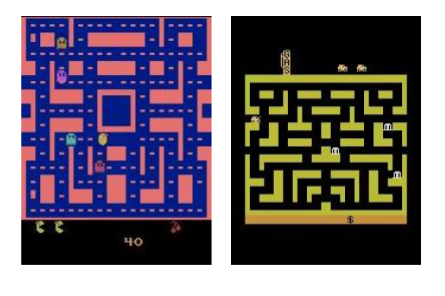
\includegraphics[width=\textwidth]{./figures/similar_sources}
	\caption{The visually similar \texttt{Ms Pacman} and \texttt{Bank Heist} games.}
	\label{fig:similar_games}
	\end{minipage}
	\hspace{0.5cm}
	\begin{minipage}[b]{0.45\linewidth}
	\centering
	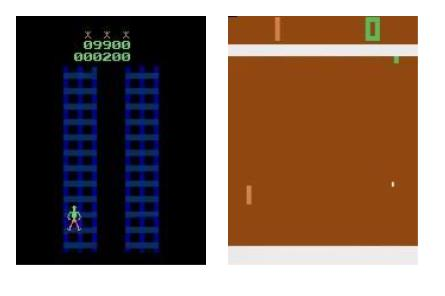
\includegraphics[width=\textwidth]{./figures/dissimilar_sources}
	\caption{The highly different \texttt{Crazy Climber} and \texttt{Pong} games.}
	\label{fig:dissimilar_games}
	\end{minipage}
	\end{figure}
	\end{frame}

\begin{frame}{On the Transferability of Deep-Q Networks}

	We quantitatively measure the benefits of transferring and fine-tuning a pre-trained model by computing the \textcolor{RoyalBlue}{area ratio metric} \footnote{Lazaric, Alessandro. "Transfer in reinforcement learning: a framework and a survey." Reinforcement Learning. Springer (2012).} $\mathscr{R}$

	\begin{equation*}
		\mathscr{R} = \frac{\text{area of $\mathcal{M}_S$ $-$ area of $\mathcal{M}_T$}}{\text{area of $\mathcal{M}_T$}}
	\label{eq:area_ratio_metric}
	\end{equation*}

	\bigskip
	expecting mostly positive values for $\mathscr{R}$

\end{frame}

\begin{frame}{On the Transferability of Deep-Q Networks}

	\bigskip

	However, we noticed that adopting Transfer Learning strategies performed \textcolor{Maroon}{surprisingly bad}

	\begin{table}[t!]
	{\newcommand*{\MinNumber}{-1}%
\newcommand*{\MaxNumber}{1}%

\newcommand{\ApplyGradient}[1]{%
  \pgfmathsetmacro{\PercentColor}{100.0*(#1-\MaxNumber)/(\MinNumber-\MaxNumber)}%
  %\textcolor{black!\PercentColor}{#1}
  \edef\x{\noexpand\cellcolor{red!\PercentColor}}\x\textcolor{black}{#1}%
}
\newcolumntype{R}{>{\collectcell\ApplyGradient}{c}<{\endcollectcell}}

\resizebox{\columnwidth}{!}{%
\begin{tabular}{c|R|R|R|R|R|R|R|R|R|R}
\hline 
{} & BankHeist & Boxing & CrazyClimber & Enduro & FishingDerby & Frostbite & JamesBond & MsPacman &   Pong & Zaxxon \\
\hline \hline 
BankHeist    &     -      & -0.019 &           -1 & -0.317 &          0.5 &     0.729 &     0.973 &   -0.089 & -1.238 & -0.998 \\
Boxing       &    -0.494 &    -    &       -0.278 & -0.852 &        0.552 &     -0.01 &     0.247 &   -0.184 & -0.841 & -0.999 \\
CrazyClimber &    -0.569 & -0.261 &           -   & -0.593 &         0.19 &     0.277 &     0.621 &   -0.111 & -1.206 & -0.178 \\
Enduro       &    -0.571 & -0.018 &        -0.25 &     -   &        0.726 &    -0.017 &     -0.41 &    -0.08 & -0.466 & -0.164 \\
FishingDerby &        -1 & -0.893 &       -0.093 &  -0.45 &            -  &     0.068 &     0.197 &   -0.136 & -3.083 & -0.999 \\
Frostbite    &    -0.933 &  0.024 &           -1 & -0.348 &        0.222 &        -   &     0.569 &    0.009 & -0.663 & -0.076 \\
JamesBond    &    -0.123 & -0.106 &       -0.131 & -0.033 &        0.519 &     0.262 &         -  &    0.218 & -1.329 &     -1 \\
MsPacman     &    -0.985 & -0.219 &       -0.012 & -0.494 &          0.6 &     0.346 &     0.398 &        -  & -1.646 & -0.997 \\
Pong         &        -1 & -0.083 &       -0.428 & -0.476 &        0.725 &    -0.024 &     0.896 &    0.123 &    -    & -0.729 \\
Zaxxon       &     -0.76 & -0.028 &        0.037 & -0.116 &        0.385 &      0.16 &    -0.253 &     0.06 & -1.602 &   -     \\
\end{tabular}%
}

}
	\label{tab:dqv_res}
%\end{table}


%\begin{table}[ht!]
        %	\caption{The results obtained when fine-tuning ten different pre-trained DDQN agents (rows) on nine other Atari games (columns). Similarly to Table \ref{tab:dqv_res} the lower the area ratio score, the redder the color of the cell.} %We can again observe that fine-tuning a pre-trained agent is only beneficial in a very limited number of cases and that the DDQN algorithm results in different transfer learning performance than DQV.}
        ~\\
	{\newcommand*{\MinNumber}{-1}%
\newcommand*{\MaxNumber}{1}%

\newcommand{\ApplyGradient}[1]{%
  \pgfmathsetmacro{\PercentColor}{100.0*(#1-\MaxNumber)/(\MinNumber-\MaxNumber)}%
  %\textcolor{black!\PercentColor}{#1}
  \edef\x{\noexpand\cellcolor{red!\PercentColor}}\x\textcolor{black}{#1}%
}
\newcolumntype{R}{>{\collectcell\ApplyGradient}{c}<{\endcollectcell}}

\resizebox{\columnwidth}{!}{%
\begin{tabular}{c|R|R|R|R|R|R|R|R|R|R}
\hline 
{} & BankHeist & Boxing & CrazyClimber & Enduro & FishingDerby & Gopher & IceHockey & Jamesbond & MsPacman & Pong \\
\hline\hline
BankHeist    &       -                    &                  0.121 &                       -0.378 &                 -0.006 &                       -0.107 &                  0.042 &                    -0.006 &                    -0.058 &                    0.001 &               -3.013 \\
Boxing       &                    -0.316 &     -                   &                       -0.104 &                     -0 &                        0.038 &                   0.06 &                     0.015 &                    -0.225 &                   -0.027 &                0.936 \\
CrazyClimber &                    -0.192 &                 -0.487 &               -               &                 -0.012 &                       -0.084 &                  0.016 &                     0.015 &                     0.016 &                   -0.015 &                -2.64 \\
Enduro       &                    -0.296 &                  0.193 &                       -0.167 &       -                 &                        0.039 &                   0.03 &                     0.019 &                    -0.235 &                   -0.039 &                0.248 \\
FishingDerby &                    -0.212 &                 -0.545 &                           -1 &                 -0.085 &         -                     &                  0.016 &                     0.001 &                    -0.055 &                   -0.026 &               -0.935 \\
Gopher       &                    -0.466 &                  0.044 &                       -0.108 &                 -0.005 &                        0.007 &            -            &                    -0.005 &                    -0.094 &                    -0.02 &               -1.816 \\
IceHockey    &                    -0.046 &                  0.245 &                       -0.067 &                  0.014 &                       -0.178 &                  0.072 &            -               &                     0.037 &                   -0.015 &                0.112 \\
Jamesbond    &                    -0.145 &                  0.232 &                       -0.064 &                  0.005 &                       -0.267 &                  0.031 &                    -0.092 &      -                     &                   -0.006 &               -1.578 \\
MsPacman     &                    -0.173 &                 -1.179 &                       -0.129 &                  -0.06 &                        0.003 &                 -0.019 &                     0.007 &                     0.071 &       -                   &               -2.774 \\
Pong         &                    -0.127 &                  0.028 &                        -0.12 &                   0.01 &                        0.037 &                  0.042 &                     0.002 &                    -0.174 &                   -0.006 &             -         \\
\end{tabular}%
}
}
	\label{tab:ddqn_res}
\end{table}

\end{frame}


\begin{frame}{On the Transferability of Deep-Q Networks}

	Specifically, on the \texttt{Atari} benchmark we have noticed that:
	\bigskip
	\begin{itemize}
		\item Transferring pre-trained Deep-Q Networks mostly results in \textcolor{Maroon}{negative transfer}, even across similar games \texttt{Bank Heist} $\rightarrow$ \texttt{Ms. Pacman}
		\item Transfer across environments is \textcolor{Maroon}{not symmetric}: \texttt{Bank Heist} $\leftrightarrow$ \texttt{Fishing Derby}
		\item Different algorithms result in \textcolor{Maroon}{different} transfer learning performance
	\end{itemize}

	\bigskip

	$\Rightarrow$ Can we \textcolor{RoyalBlue}{explain} these results any further?

\end{frame}

\begin{frame}{On the Transferability of Deep-Q Networks}
	\bigskip
	We have designed a set of novel \textcolor{RoyalBlue}{control tasks} that could help us better understanding the transfer learning potential of Deep-Q Networks 
	\bigskip
	\begin{figure}[ht]
\begin{minipage}{0.5\textwidth}
	\centering
	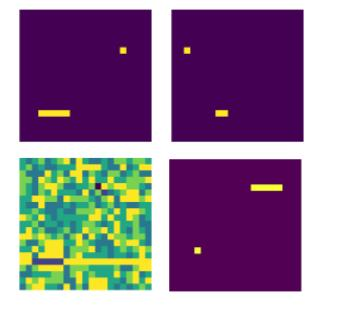
\includegraphics[width=5cm]{./figures/catch_games}
\end{minipage}%
\begin{minipage}{0.5\textwidth}
	\centering
	\begin{tikzpicture}
\begin{axis}
[	grid style={dashed,gray},
	grid = both, 
	tick style=black,
  	xlabel=Epochs,
	ylabel = $\%$ of caught balls,
	legend style={at={(-0.3,-0.3,-0.4)},anchor=south west,legend columns=4},
]

\addlegendentry{\texttt{Catch-v0}}

\addplot[blue, ultra thick] table[x=epochs,y=catchv0] {./Results/Chapter08/logs/catch_baselines.dat};
\addplot[name path=upper,draw=none, forget plot] table[x=epochs,y expr=\thisrow{catchv0}+\thisrow{stdv0}] {./Results/Chapter08/logs/catch_baselines.dat};
\addplot[name path=lower,draw=none, forget plot] table[x=epochs,y expr=\thisrow{catchv0}-\thisrow{stdv0}] {./Results/Chapter08/logs/catch_baselines.dat};
\addplot[fill=blue!10, forget plot] fill between[of=upper and lower];

\addlegendentry{\texttt{Catch-v1}}
\addplot[ultra thick, yellow] table[x=epochs,y=catchv3] {./Results/Chapter08/logs/catch_baselines.dat};
\addplot [name path=upper,draw=none, forget plot] table[x=epochs,y expr=\thisrow{catchv3}+\thisrow{stdv3}] {./Results/Chapter08/logs/catch_baselines.dat};
\addplot [name path=lower,draw=none, forget plot] table[x=epochs,y expr=\thisrow{catchv3}-\thisrow{stdv3}] {./Results/Chapter08/logs/catch_baselines.dat};
\addplot [fill=yellow!10, forget plot] fill between[of=upper and lower];

\addlegendentry{\texttt{Catch-v2}}
\addplot[ultra thick, red] table[x=epochs,y=catchv1] {./Results/Chapter08/logs/catch_baselines.dat};
\addplot[name path=upper,draw=none, forget plot] table[x=epochs,y expr=\thisrow{catchv1}+\thisrow{stdv1}] {./Results/Chapter08/logs/catch_baselines.dat};
\addplot[name path=lower,draw=none, forget plot] table[x=epochs,y expr=\thisrow{catchv1}-\thisrow{stdv1}] {./Results/Chapter08/logs/catch_baselines.dat};
\addplot[fill=red!10, forget plot] fill between[of=upper and lower];

\addlegendentry{\texttt{Catch-v3}}
\addplot[ultra thick, green] table[x=epochs,y=catchv2] {./Results/Chapter08/logs/catch_baselines.dat};
\addplot [name path=upper,draw=none, forget plot] table[x=epochs,y expr=\thisrow{catchv2}+\thisrow{stdv2}] {./Results/Chapter08/logs/catch_baselines.dat};
\addplot [name path=lower,draw=none, forget plot] table[x=epochs,y expr=\thisrow{catchv2}-\thisrow{stdv2}] {./Results/Chapter08/logs/catch_baselines.dat};
\addplot [fill=green!10, forget plot] fill between[of=upper and lower];

\end{axis}
\end{tikzpicture}


\end{minipage}
\label{fig:catch_baselines}
\end{figure}

\end{frame}

\begin{frame}{On the Transferability of Deep-Q Networks}

	\bigskip
	$\Rightarrow$ Even on our newly designed problems, we keep observing \textcolor{Maroon}{very poor} transfer learning performance
	\bigskip
\begin{table}[ht!]
	\centering
	%\caption{The area ratio obtained after fine-tuning a pre-trained DQN agent on the different \texttt{Catch} environments. We can see that no matter which source game is used for pre-training, transfer learning surprisingly never results in positive transfer.}
	\newcommand*{\MinNumber}{-0.479}%
\newcommand*{\MaxNumber}{0.1}%

\newcommand{\ApplyGradient}[1]{%
  \pgfmathsetmacro{\PercentColor}{100.0*(#1-\MaxNumber)/(\MinNumber-\MaxNumber)}%
  %\textcolor{black!\PercentColor}{#1}
  \edef\x{\noexpand\cellcolor{red!\PercentColor}}\x\textcolor{black}{#1}%
}
\newcolumntype{R}{>{\collectcell\ApplyGradient}{c}<{\endcollectcell}}
\begin{tabular}{c|R|R|R|R}
\hline 
{} & Catch-v0 & Catch-v2 & Catch-v3 & Catch-v4 \\ \hline\hline
Catch-v0 &       -   &   -0.026 &   -0.486 &   -0.479 \\
Catch-v2 &    -0.16 &       -   &   -0.121 &   -0.248 \\
Catch-v3 &   -0.406 &   -0.313 &      -    &   -0.465 \\
Catch-v4 &   -0.016 &    -0.24 &   -0.179 &       -   \\
\end{tabular}

	\label{tab:catch_tl_area_ratio}
\end{table}

\end{frame}

\begin{frame}{On the Transferability of Deep-Q Networks}
	
	\bigskip
	We therefore asked ourselves whether Deep-Q Networks are at least able to \textcolor{RoyalBlue}{self-transfer} ...
	\bigskip
	\begin{itemize}
		\item What happens when the source task $\mathcal{M}_S$ and the target task $\mathcal{M}_T$ are identical?
		\item Are there any differences between using an off-the-shelf approach compared to a fine-tuning strategy?
		\item Let's recall that when transferring a pre-trained model only the last layer responsible for estimating $Q(s,a)$ is randomly initialized
	\end{itemize}

\end{frame}

\begin{frame}{On the Transferability of Deep-Q Networks}
	
	We notice that positive self-transfer can get obtained as long as the networks \textcolor{Maroon}{do not get fine-tuned} but are used as feature extractors instead

	\begin{table}[ht!]
	\centering
%	\caption{The area ratio scores obtained after performing self-transfer. We can see that if only the last linear layer is trained, then positive transfer is obtained on all \texttt{Catch} environments, whereas if the network is fine-tuned, positive transfer is (in part) only obtained on \texttt{Catch-v2}.}
	\newcommand*{\MinNumber}{-0.236}%
\newcommand*{\MaxNumber}{0.674}%

\newcommand{\ApplyGradient}[1]{%
  \pgfmathsetmacro{\PercentColor}{100.0*(#1-\MaxNumber)/(\MinNumber-\MaxNumber)}%
  %\textcolor{black!\PercentColor}{#1}
  \edef\x{\noexpand\cellcolor{red!\PercentColor}}\x\textcolor{black}{#1}%
}
\newcolumntype{R}{>{\collectcell\ApplyGradient}{c}<{\endcollectcell}}
\begin{tabular}{c|R|R|R|R}
\hline 
           &  Catch-v0 & Catch-v1 & Catch-v2 & Catch-v3 \\ \hline \hline
Only-Head   & 0.05     & 0.141    & 0.674    & 0.059    \\
Fine-Tuning & 0.017    & -0.218   & 0.393    & -0.236   \\   
\end{tabular}	

	\label{tab:self_tl_area_ratio}
	\end{table}

\end{frame}

\begin{frame}{On the Transferability of Deep-Q Networks}

	\bigskip
	Our \textcolor{RoyalBlue}{conjecture} is that a Deep-Q Network can only solve a problem if it has carefully found a balance between its feature extractor components and the linear layer that estimates $Q(s,a)$

	\bigskip

	\begin{figure}[ht!]
\resizebox{0.60\textwidth}{!}{
\begin{tikzpicture}
\begin{axis}
[	
	name=ax1,	
	grid style={dashed,gray},
	grid = both, 
	tick style=black,
  	xlabel=Epochs,
	ylabel = $\%$ of caught balls,
	title = \texttt{Catch-v1},
	legend pos=south east,	
]


\addlegendentry{\texttt{Catch-v1}}
\addplot[yellow, ultra thick] table[x=epochs,y=baseline] {./Chapter08/logs/self_transfer_catch_v1.dat};
\addplot [name path=upper,draw=none, forget plot] table[x=epochs,y expr=\thisrow{baseline}+\thisrow{std_baseline}] {./Chapter08/logs/self_transfer_catch_v1.dat};
\addplot [name path=lower,draw=none, forget plot] table[x=epochs,y expr=\thisrow{baseline}-\thisrow{std_baseline}] {./Chapter08/logs/self_transfer_catch_v1.dat};
\addplot [fill=yellow!10, forget plot] fill between[of=upper and lower];

\iffalse
\addlegendentry{Fine-Tuning}
\addplot[dashed, ultra thick,yellow] table[x=epochs,y=self_transfer_full_fine_tuning] {./Chapter08/logs/hybrid_self_tl_v1.dat};
\addplot [name path=upper,draw=none, forget plot] table[x=epochs,y expr=\thisrow{self_transfer_full_fine_tuning}+\thisrow{std_self_transfer_full_fine_tuning}] {./Chapter08/logs/hybrid_self_tl_v1.dat};
\addplot [name path=lower,draw=none, forget plot] table[x=epochs,y expr=\thisrow{self_transfer_full_fine_tuning}-\thisrow{std_self_transfer_full_fine_tuning}] {./Chapter08/logs/hybrid_self_tl_v1.dat};
\addplot [fill=yellow!10, forget plot] fill between[of=upper and lower];

\addlegendentry{Hybrid Fine-Tuning}
\addplot[dashed, ultra thick,cyan] table[x=epochs,y=hybrid_self_transfer] {./Chapter08/logs/hybrid_self_tl_v1.dat};
\addplot [name path=upper,draw=none, forget plot] table[x=epochs,y expr=\thisrow{hybrid_self_transfer}+\thisrow{std_hybrid_self_transfer}] {./Chapter08/logs/hybrid_self_tl_v1.dat};
\addplot [name path=lower,draw=none, forget plot] table[x=epochs,y expr=\thisrow{hybrid_self_transfer}-\thisrow{std_hybrid_self_transfer}] {./Chapter08/logs/hybrid_self_tl_v1.dat};
\addplot [fill=cyan!10, forget plot] fill between[of=upper and lower];
\fi

\end{axis}

\end{tikzpicture}%
}
\end{figure}


\end{frame}

\begin{frame}{On the Transferability of Deep-Q Networks}

	\bigskip
	Our \textcolor{RoyalBlue}{conjecture} is that a Deep-Q Network can only solve a problem if it has carefully found a balance between its feature extractor components and the linear layer that estimates $Q(s,a)$

	\bigskip

	\begin{figure}[ht!]
\resizebox{0.60\textwidth}{!}{
\begin{tikzpicture}
\begin{axis}
[	
	name=ax1,	
	grid style={dashed,gray},
	grid = both, 
	tick style=black,
  	xlabel=Epochs,
	ylabel = $\%$ of caught balls,
	title = \texttt{Catch-v1},
	legend pos=south east,	
]


\addlegendentry{\texttt{Catch-v1}}
\addplot[yellow, ultra thick] table[x=epochs,y=baseline] {./Chapter08/logs/self_transfer_catch_v1.dat};
\addplot [name path=upper,draw=none, forget plot] table[x=epochs,y expr=\thisrow{baseline}+\thisrow{std_baseline}] {./Chapter08/logs/self_transfer_catch_v1.dat};
\addplot [name path=lower,draw=none, forget plot] table[x=epochs,y expr=\thisrow{baseline}-\thisrow{std_baseline}] {./Chapter08/logs/self_transfer_catch_v1.dat};
\addplot [fill=yellow!10, forget plot] fill between[of=upper and lower];


\addlegendentry{Fine-Tuning}
\addplot[dashed, ultra thick,yellow] table[x=epochs,y=self_transfer_full_fine_tuning] {./Chapter08/logs/hybrid_self_tl_v1.dat};
\addplot [name path=upper,draw=none, forget plot] table[x=epochs,y expr=\thisrow{self_transfer_full_fine_tuning}+\thisrow{std_self_transfer_full_fine_tuning}] {./Chapter08/logs/hybrid_self_tl_v1.dat};
\addplot [name path=lower,draw=none, forget plot] table[x=epochs,y expr=\thisrow{self_transfer_full_fine_tuning}-\thisrow{std_self_transfer_full_fine_tuning}] {./Chapter08/logs/hybrid_self_tl_v1.dat};
\addplot [fill=yellow!10, forget plot] fill between[of=upper and lower];

\iffalse
\addlegendentry{Hybrid Fine-Tuning}
\addplot[dashed, ultra thick,cyan] table[x=epochs,y=hybrid_self_transfer] {./Chapter08/logs/hybrid_self_tl_v1.dat};
\addplot [name path=upper,draw=none, forget plot] table[x=epochs,y expr=\thisrow{hybrid_self_transfer}+\thisrow{std_hybrid_self_transfer}] {./Chapter08/logs/hybrid_self_tl_v1.dat};
\addplot [name path=lower,draw=none, forget plot] table[x=epochs,y expr=\thisrow{hybrid_self_transfer}-\thisrow{std_hybrid_self_transfer}] {./Chapter08/logs/hybrid_self_tl_v1.dat};
\addplot [fill=cyan!10, forget plot] fill between[of=upper and lower];
\fi

\end{axis}

\end{tikzpicture}%
}
\end{figure}


\end{frame}

\begin{frame}{On the Transferability of Deep-Q Networks}

	\bigskip
	Our \textcolor{RoyalBlue}{conjecture} is that a Deep-Q Network can only solve a problem if it has carefully found a balance between its feature extractor components and the linear layer that estimates $Q(s,a)$

	\bigskip

	\begin{figure}[ht!]
  \centering

\resizebox{\columnwidth}{!}{%
\begin{tikzpicture}
\begin{axis}
[	
	name=ax1,	
	grid style={dashed,gray},
	grid = both, 
	tick style=black,
  	xlabel=Epochs,
	ylabel = $\%$ of caught balls,
	title = \texttt{Catch-v0},
	legend pos=south east,	
]

\addlegendentry{\texttt{Catch-v0}}
\addplot[blue, ultra thick] table[x=epochs,y=baseline] {./Results/Chapter08/logs/hybrid_self_tl_v0.dat};
\addplot [name path=upper,draw=none] table[x=epochs,y expr=\thisrow{baseline}+\thisrow{std_baseline}] {./Results/Chapter08/logs/hybrid_self_tl_v0.dat};
\addplot [name path=lower,draw=none] table[x=epochs,y expr=\thisrow{baseline}-\thisrow{std_baseline}] {./Results/Chapter08/logs/hybrid_self_tl_v0.dat};
\addplot [fill=blue!10] fill between[of=upper and lower];


\addlegendentry{\texttt{Full Fine-Tuning}}
\addplot[dashed, ultra thick,blue] table[x=epochs,y=self_transfer_full_fine_tuning] {./Results/Chapter08/logs/hybrid_self_tl_v0.dat};
\addplot [name path=upper,draw=none] table[x=epochs,y expr=\thisrow{self_transfer_full_fine_tuning}+\thisrow{std_self_transfer_full_fine_tuning}] {./Results/Chapter08/logs/hybrid_self_tl_v0.dat};
\addplot [name path=lower,draw=none] table[x=epochs,y expr=\thisrow{self_transfer_full_fine_tuning}-\thisrow{std_self_transfer_full_fine_tuning}] {./Results/Chapter08/logs/hybrid_self_tl_v0.dat};
\addplot [fill=blue!10] fill between[of=upper and lower];

\addlegendentry{\texttt{Hybrid Fine-Tuning}}
\addplot[dashed, ultra thick,gray] table[x=epochs,y=hybrid_self_transfer] {./Results/Chapter08/logs/hybrid_self_tl_v0.dat};
\addplot [name path=upper,draw=none] table[x=epochs,y expr=\thisrow{hybrid_self_transfer}+\thisrow{std_hybrid_self_transfer}] {./Results/Chapter08/logs/hybrid_self_tl_v0.dat};
\addplot [name path=lower,draw=none] table[x=epochs,y expr=\thisrow{hybrid_self_transfer}-\thisrow{std_hybrid_self_transfer}] {./Results/Chapter08/logs/hybrid_self_tl_v0.dat};
\addplot [fill=gray!10] fill between[of=upper and lower];


\end{axis}


\begin{axis}
[	
	at={(ax1.south east)},
	xshift=2cm,	
	grid style={dashed,gray},
	grid = both, 
	tick style=black,
  	xlabel=Epochs,
	ylabel = $\%$ of caught balls,
	title = \texttt{Catch-v1},
	legend pos=south east,	
]

\addlegendentry{\texttt{Catch-v1}}
\addplot[yellow, ultra thick] table[x=epochs,y=baseline] {./Results/Chapter08/logs/hybrid_self_tl_v1.dat};
\addplot [name path=upper,draw=none] table[x=epochs,y expr=\thisrow{baseline}+\thisrow{std_baseline}] {./Results/Chapter08/logs/hybrid_self_tl_v1.dat};
\addplot [name path=lower,draw=none] table[x=epochs,y expr=\thisrow{baseline}-\thisrow{std_baseline}] {./Results/Chapter08/logs/hybrid_self_tl_v1.dat};
\addplot [fill=yellow!10] fill between[of=upper and lower];


\addlegendentry{\texttt{Full Fine-Tuning}}
\addplot[dashed, ultra thick,yellow] table[x=epochs,y=self_transfer_full_fine_tuning] {./Results/Chapter08/logs/hybrid_self_tl_v1.dat};
\addplot [name path=upper,draw=none] table[x=epochs,y expr=\thisrow{self_transfer_full_fine_tuning}+\thisrow{std_self_transfer_full_fine_tuning}] {./Results/Chapter08/logs/hybrid_self_tl_v1.dat};
\addplot [name path=lower,draw=none] table[x=epochs,y expr=\thisrow{self_transfer_full_fine_tuning}-\thisrow{std_self_transfer_full_fine_tuning}] {./Results/Chapter08/logs/hybrid_self_tl_v1.dat};
\addplot [fill=yellow!10] fill between[of=upper and lower];

\addlegendentry{\texttt{Hybrid Fine-Tuning}}
\addplot[dashed, ultra thick,gray] table[x=epochs,y=hybrid_self_transfer] {./Results/Chapter08/logs/hybrid_self_tl_v1.dat};
\addplot [name path=upper,draw=none] table[x=epochs,y expr=\thisrow{hybrid_self_transfer}+\thisrow{std_hybrid_self_transfer}] {./Results/Chapter08/logs/hybrid_self_tl_v1.dat};
\addplot [name path=lower,draw=none] table[x=epochs,y expr=\thisrow{hybrid_self_transfer}-\thisrow{std_hybrid_self_transfer}] {./Results/Chapter08/logs/hybrid_self_tl_v1.dat};
\addplot [fill=gray!10] fill between[of=upper and lower];


\end{axis}


\end{tikzpicture}%
}



 \resizebox{\columnwidth}{!}{%
\begin{tikzpicture}
\begin{axis}
[	
	name=ax1,	
	grid style={dashed,gray},
	grid = both, 
	tick style=black,
  	xlabel=Epochs,
	ylabel = $\%$ of caught balls,
	title = \texttt{Catch-v2},
	legend pos=south east,	
]

\addlegendentry{\texttt{Catch-v2}}
\addplot[red, ultra thick] table[x=epochs,y=baseline] {./Results/Chapter08/logs/hybrid_self_tl_v2.dat};
\addplot [name path=upper,draw=none] table[x=epochs,y expr=\thisrow{baseline}+\thisrow{std_baseline}] {./Results/Chapter08/logs/hybrid_self_tl_v2.dat};
\addplot [name path=lower,draw=none] table[x=epochs,y expr=\thisrow{baseline}-\thisrow{std_baseline}] {./Results/Chapter08/logs/hybrid_self_tl_v2.dat};
\addplot [fill=red!10] fill between[of=upper and lower];


\addlegendentry{\texttt{Full Fine-Tuning}}
\addplot[dashed, ultra thick,red] table[x=epochs,y=self_transfer_full_fine_tuning] {./Results/Chapter08/logs/hybrid_self_tl_v2.dat};
\addplot [name path=upper,draw=none] table[x=epochs,y expr=\thisrow{self_transfer_full_fine_tuning}+\thisrow{std_self_transfer_full_fine_tuning}] {./Results/Chapter08/logs/hybrid_self_tl_v2.dat};
\addplot [name path=lower,draw=none] table[x=epochs,y expr=\thisrow{self_transfer_full_fine_tuning}-\thisrow{std_self_transfer_full_fine_tuning}] {./Results/Chapter08/logs/hybrid_self_tl_v2.dat};
\addplot [fill=red!10] fill between[of=upper and lower];


\addlegendentry{\texttt{Hybrid Fine-Tuning}}
\addplot[dashed, ultra thick,gray] table[x=epochs,y=hybrid_self_transfer] {./Results/Chapter08/logs/hybrid_self_tl_v2.dat};
\addplot [name path=upper,draw=none] table[x=epochs,y expr=\thisrow{hybrid_self_transfer}+\thisrow{std_hybrid_self_transfer}] {./Results/Chapter08/logs/hybrid_self_tl_v2.dat};
\addplot [name path=lower,draw=none] table[x=epochs,y expr=\thisrow{hybrid_self_transfer}-\thisrow{std_hybrid_self_transfer}] {./Results/Chapter08/logs/hybrid_self_tl_v2.dat};
\addplot [fill=gray!10] fill between[of=upper and lower];

\end{axis}


\begin{axis}
[	
	at={(ax1.south east)},
	xshift=2cm,	
	grid style={dashed,gray},
	grid = both, 
	tick style=black,
  	xlabel=Epochs,
	ylabel = $\%$ of caught balls,
	title = \texttt{Catch-v3},
	legend pos=south east,	
]

\addlegendentry{\texttt{Catch-v0}}
\addplot[green, ultra thick] table[x=epochs,y=baseline] {./Results/Chapter08/logs/hybrid_self_tl_v3.dat};
\addplot [name path=upper,draw=none] table[x=epochs,y expr=\thisrow{baseline}+\thisrow{std_baseline}] {./Results/Chapter08/logs/hybrid_self_tl_v3.dat};
\addplot [name path=lower,draw=none] table[x=epochs,y expr=\thisrow{baseline}-\thisrow{std_baseline}] {./Results/Chapter08/logs/hybrid_self_tl_v3.dat};
\addplot [fill=green!10] fill between[of=upper and lower];


\addlegendentry{\texttt{Full Fine-Tuning}}
\addplot[dashed, ultra thick,green] table[x=epochs,y=self_transfer_full_fine_tuning] {./Results/Chapter08/logs/hybrid_self_tl_v3.dat};
\addplot [name path=upper,draw=none] table[x=epochs,y expr=\thisrow{self_transfer_full_fine_tuning}+\thisrow{std_self_transfer_full_fine_tuning}] {./Results/Chapter08/logs/hybrid_self_tl_v3.dat};
\addplot [name path=lower,draw=none] table[x=epochs,y expr=\thisrow{self_transfer_full_fine_tuning}-\thisrow{std_self_transfer_full_fine_tuning}] {./Results/Chapter08/logs/hybrid_self_tl_v3.dat};
\addplot [fill=green!10] fill between[of=upper and lower];

\addlegendentry{\texttt{Hybrid Fine-Tuning}}
\addplot[dashed, ultra thick,gray] table[x=epochs,y=hybrid_self_transfer] {./Results/Chapter08/logs/hybrid_self_tl_v3.dat};
\addplot [name path=upper,draw=none] table[x=epochs,y expr=\thisrow{hybrid_self_transfer}+\thisrow{std_hybrid_self_transfer}] {./Results/Chapter08/logs/hybrid_self_tl_v3.dat};
\addplot [name path=lower,draw=none] table[x=epochs,y expr=\thisrow{hybrid_self_transfer}-\thisrow{std_hybrid_self_transfer}] {./Results/Chapter08/logs/hybrid_self_tl_v3.dat};
\addplot [fill=gray!10] fill between[of=upper and lower];

\end{axis}


\end{tikzpicture}%
}
\caption{The results of our self-transfer experiments. In clockwise order the performance obtained on \texttt{Catchv-0}, \texttt{Catch-v1}, \texttt{Catch-v2} and \texttt{Catch-v3} after either training only the last linear layer of a pre-trained Deep-Q Network (dotted lines), or after wholly fine-tuning the model (dashed lines). We can see that the former transfer learning strategy yields significantly better results and that a fine-tuning approach results in networks that in three cases out of four are not even able to transfer to themselves.}
\label{fig:hybrid_self_transfer}
\end{figure}


\end{frame}


\begin{frame}{On the Transferability of Deep-Q Networks}
	
	Takeaway of PART III ...
	\bigskip
	\begin{itemize}
		\item We show that fine-tuning pre-trained models in a model-free Deep Reinforcement Learning context is \textcolor{Maroon}{particularly challenging} 
		\item There is a clear \textcolor{Maroon}{difference} in terms of performance with the results presented in PART II
		\item We provide some \textcolor{RoyalBlue}{initial intuition} about why negative transfer seems to be happening
		\item This remains an \textcolor{RoyalBlue}{open problem} that we believe deserves attention
	\end{itemize}

\end{frame}


\begin{frame}{Conclusion}

	\bigskip
	\begin{center}
		\textcolor{skymagenta}{\textbf{Future Work}}
	\end{center}

	\bigskip
	\begin{itemize}
		\item A Transfer Learning study of Vision Transformers (ViTs) \footnote{Dosovitskiy, Alexey, et al. "An image is worth 16x16 words: Transformers for image recognition at scale." arXiv preprint arXiv:2010.11929 (2020).}
		\item Consider alternative training approaches such as meta-learning and multi-task learning 
		\item Focus on deep model-based Reinforcement Learning
	\end{itemize}


\end{frame}

\begin{frame}
	\begin{center}
		\textcolor{skymagenta}{\textbf{The End.}}
	\end{center}
\end{frame}

\begin{frame}{Final References}
	\begin{itemize}
		\fontsize{6pt}{7.2}\selectfont
		\item Sabatelli, Matthia, et al. "Deep transfer learning for art classification problems." Proceedings of the European Conference on Computer Vision (ECCV) Workshops. 2018.
		\item Sabatelli, Matthia, et al. "Advances in Digital Music Iconography: Benchmarking the detection of musical instruments in unrestricted, non-photorealistic images from the artistic domain." Digital Humanities Quarterly 15.1 (2021).
		\item Sabatelli, Matthia, Mike Kestemont, and Pierre Geurts. "On the Transferability of Winning Tickets in Non-natural Image Datasets." VISIGRAPP (5: VISAPP). 2021.
		\item Sabatelli, Matthia, et al. "Deep Quality Value (DQV) Learning." Deep Reinforcement Learning Workshop of the 32nd Conference on Neural Information Processing Systems (2018).
		\item Sabatelli, Matthia, et al. "The deep quality-value family of deep reinforcement learning algorithms." 2020 International Joint Conference on Neural Networks (IJCNN). IEEE, 2020.
		\item Sabatelli, Matthia, and Pierre Geurts. "On The Transferability of Deep-Q Networks." Deep Reinforcement Learning Workshop of the 35th Conference on Neural Information Processing Systems. 2021.
	\end{itemize}

\end{frame}

%============================================================================


\appendix

\begin{frame}{Backup}
	\bigskip
	\textit{"Why not transfer fully pre-trained pruned models $f(x,m\odot\theta_i)$ instead of lottery tickets $f(x,m\odot\theta_k)$?"}
	\bigskip
	\begin{figure}[ht!]
\centering
	\begin{tikzpicture}[scale = 0.3]

\begin{axis}[
	name=ax1,
	grid style={dashed,gray},
	grid = both, 
	tick style=black,
  	x label style={at={(axis description cs:0.5,-0.1)},anchor=north},
	xlabel=Fraction of Weights Pruned,
  	ylabel= Accuracy ($\%$),
	title=Human-LBA,
	%width=1,
	xtick=data,
	label style={font=\scriptsize},
	xticklabels = {0.0,0.2,0.36,0.488,0.59,0.672,0.738,0.79,0.832,0.866,0.893,0.914,0.931,0.945,0.956,0.965,0.972,0.977,0.982,0.986,0.988,0.991,0.993,0.994,0.995,0.996,0.997,0.998,0.998,0.998,0.999},
	x=4.5mm,
	ymin=40,
    	ymax=90,
	scale only axis,
	xticklabel style={rotate=90},
        %log ticks with fixed point,
        scaled ticks=true,
	/pgf/number format/fixed,
        %log ticks with fixed point,
  	legend pos= north east,
	%legend style={font=\small, at={(-0.8,-0.2,-0.2)},anchor=north west, legend columns = 1}
	]

	\addlegendentry{Baseline}
	\addlegendentry{Winning Ticket $f(x;m\odot\theta_k)$}
	\addlegendentry{CIFAR-10 $f(x;m\odot\theta_i)$}
	
\addplot [ultra thick, black, mark=x] table [x expr=\coordindex, y=baseline]{./Chapter06/logs/human_lba_fine_tuning_study.txt};
\addplot [ultra thick, green, mark=x] table [x expr=\coordindex, y=winning_ticket]{./Chapter06/logs/human_lba_fine_tuning_study.txt};
\addplot [ultra thick, green, mark=*] table [x expr=\coordindex, y=fine_tuned_pruned_model]{./Chapter06/logs/human_lba_fine_tuning_study.txt};

\end{axis}
\end{tikzpicture}
\begin{tikzpicture}[scale = 0.3]
\begin{axis}[
	at={(ax1.south east)},
	xshift=-16cm,
	yshift=-11cm,
	grid style={dashed,gray},
	grid = both, 
	tick style=black,
	x label style={at={(axis description cs:0.5,-0.1)},anchor=north},
  	xlabel=Fraction of Weights Pruned,
  	ylabel= Accuracy ($\%$),
	title=Human-LBA,
	%width=1,
	xtick=data,
	label style={font=\scriptsize},
	xticklabels = {0.0,0.2,0.36,0.488,0.59,0.672,0.738,0.79,0.832,0.866,0.893,0.914,0.931,0.945,0.956,0.965,0.972,0.977,0.982,0.986,0.988,0.991,0.993,0.994,0.995,0.996,0.997,0.998,0.998,0.998,0.999},
	x=4.5mm,
	ymin=40,
    	ymax=90,
	scale only axis,
	xticklabel style={rotate=90},
        %log ticks with fixed point,
        scaled ticks=true,
	/pgf/number format/fixed,
        %log ticks with fixed point,
  	legend pos= north east,
	%legend style={font=\Large, at={(-0.8,-0.2,-0.2)},anchor=north west, legend columns = 2}
	]

	\addlegendentry{Baseline}
	\addlegendentry{Winning Ticket $f(x;m\odot\theta_k)$}
	\addlegendentry{CIFAR-100 $f(x;m\odot\theta_i)$}
	
\addplot [ultra thick, black, mark=x] table [x expr=\coordindex, y=baseline]{./Chapter06/logs/human_lba_fine_tuning_study_cif.txt};
\addplot [ultra thick, red, mark=x] table [x expr=\coordindex, y=winning_ticket]{./Chapter06/logs/human_lba_fine_tuning_study_cif.txt};
	\addplot [ultra thick, red, mark=*] table [x expr=\coordindex, y=fine_tuned_pruned_model]{./Chapter06/logs/human_lba_fine_tuning_study_cif.txt};

\end{axis} 


    \end{tikzpicture}


\end{figure} 


\end{frame}

\begin{frame}{Backup}

	\textit{"What is the difference between the DQV-Learning algorithms and the Dueling Architecture?"} \footnote{Wang, Ziyu, et al. "Dueling network architectures for deep reinforcement learning." International conference on machine learning. PMLR, 2016.}

	\bigskip
	
	There's two main \textcolor{RoyalBlue}{differences} among e.g. DQV-Learning and the Dueling Architecture:
	\begin{enumerate}
		\item The Dueling Architecture does not explicitly learn the state-value function $V^{\pi}(s)$
		\item DQV-Learning requires two independent sets of parameters to perform well $\phi$ and $\theta$
	\end{enumerate}

\end{frame}


\begin{frame}{Backup}

	1) In the Dueling Architecture the state-value estimates and the advantage estimates are computed
	\bigskip
	\begin{multline*}
	Q(s,a;\theta^{(1)},\theta^{(2)},\theta^{(3)}) = V\bigl(s;\theta^{(1)},\theta^{(3)}\bigr) + \\
	\bigl(A(s,a;\theta^{(1)},\theta^{(2)}) - \underset{a_{t+1}\in \mathcal{A}}{\max}\: A(s, a_{t+1};\theta^{(1)},\theta^{(2)}) \bigr).
	\label{eq:dueling}
\end{multline*}
	
	 such that it is easier to train the model with DDQN's TD-target
	\bigskip
	\begin{equation*}
    y^{DDQN}_{t} = r_{t} + \gamma \: Q(s_{t+1}, \underset{a\in \mathcal{A}}{\argmax}\: Q(s_{t+1}, a; \theta); \theta^{-}). 
\end{equation*}

\end{frame}


\begin{frame}{Backup}

	1) But the true state-value function $V^{\pi}(s)$ is never explicitly learned, which \textcolor{RoyalBlue}{is the case} for DQV-Learning and DQV-Max Learning as there's a dedicated objective function for learning $\approx V^{\pi}(s;\phi)$ where we either have
	\bigskip
	\begin{multline*}
			L(\phi) = \mathds{E}_{\langle s_{t},a_{t},r_{t},s_{t+1}\rangle\sim U(D)} \bigg[\big(r_{t} + \gamma \: V(s_{t+1};\phi^{-}) - V(s_{t}; \phi)\big)^{2}\bigg],
		\end{multline*}

	\bigskip
	or
	\begin{multline*}
		L(\phi) = \mathds{E}_{\langle s_{t},a_{t},r_{t},s_{t+1}\rangle\sim U(D)} \bigg[\big(r_{t} + \gamma \: \underset{a\in \mathcal{A}}{\max}\: Q(s_{t+1}, a; \theta^{-}) - V(s_{t}; \phi)\big)^{2}\bigg],
	\end{multline*}

\end{frame}

\begin{frame}{Backup}

	2) We have also tried to train a DQV-Learning agent by following the Dueling neural architecture 
	\bigskip
	
	\begin{figure}[ht]
	\centering
	\begin{minipage}[b]{0.45\linewidth}
	\centering
	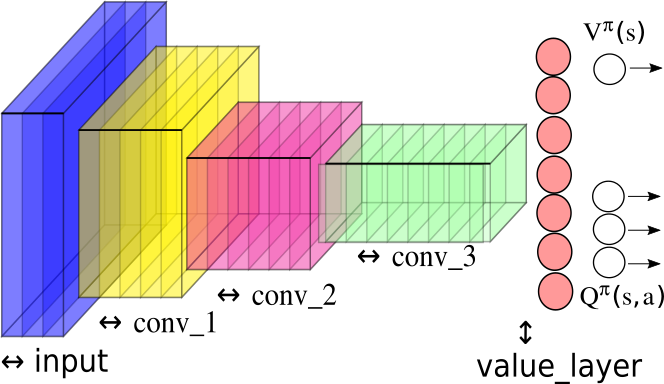
\includegraphics[width=\textwidth]{./figures/DuelingDQV_shared}
	\end{minipage}
	\hspace{0.5cm}
	\begin{minipage}[b]{0.45\linewidth}
	\centering
	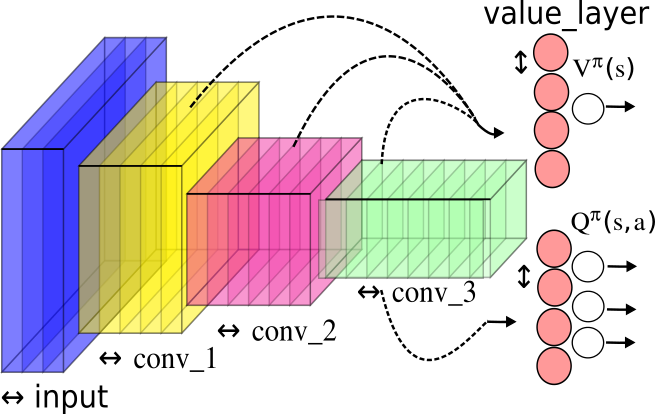
\includegraphics[width=\textwidth]{./figures/dueling_DQV}
	\end{minipage}
	\end{figure}
	\end{frame}
		
\end{frame}

\begin{frame}{Backup}

	$\Rightarrow$ But the results were \textcolor{Maroon}{never on par} with regular DQV-Learning	
	\bigskip
	\begin{figure}[ht!]
  \begin{tikzpicture}[scale = 0.65]
      \begin{axis}[
	name=ax1,
      	grid style={dashed,gray},
      	grid = both, 
      	tick style=black,
	title=Pong,
        xlabel=Episodes,
        ylabel=Reward,
      ]


      \addlegendentry{DQV}
      \addlegendentry{Duelling-DQV-1st}
      \addlegendentry{Duelling-DQV-2nd}
      \addlegendentry{Duelling-DQV-3rd}

      \addplot [ultra thick, red, mark=.] table [y=DQV, x=episodes]
      {./Results/Chapter07/logs/duelling_pong_results.txt};

      \addplot [ultra thick, green, mark=.] table [y=Duelling-DQV-1st, x=episodes]{./Results/Chapter07/logs/duelling_pong_results.txt}; 
      \addplot [ultra thick, purple, mark=.] table [y=Duelling-DQV-2nd, x=episodes]{./Results/Chapter07/logs/duelling_pong_results.txt};
      \addplot [ultra thick, cyan, mark=.] table [y=Duelling-DQV-3rd, x=episodes]{./Results/Chapter07/logs/duelling_pong_results.txt};
     
    
      \legend{}

      \end{axis}

      \begin{axis}[
	at={(ax1.south east)},
	xshift=2cm,
      	grid style={dashed,gray},
      	grid = both, 
      	tick style=black,
	title=Enduro,
        xlabel=Episodes,
        ylabel= Reward,
	legend columns=4, 
        legend style={font=\Large, at={(-0.65,-0.3,-0.4)},anchor=north west,legend columns=4},
      ]

      \addlegendentry{DQV}
      \addlegendentry{Duelling-DQV-1st}
      \addlegendentry{Duelling-DQV-2nd}
      \addlegendentry{Duelling-DQV-3rd}

      {./Results/Chapter07/logs/duelling_enduro_results.txt};
      \addplot [ultra thick, red, mark=.] table [y=DQV, x=episodes]
      {./Results/Chapter07/logs/duelling_enduro_results.txt};
      \addplot [ultra thick, green, mark=.] table [y=Duelling-DQV-1st, x=episodes]{./Results/Chapter07/logs/duelling_enduro_results.txt}; 
      \addplot [ultra thick, purple, mark=.] table [y=Duelling-DQV-2nd, x=episodes]{./Results/Chapter07/logs/duelling_pong_results.txt};
      \addplot [ultra thick, cyan, mark=.] table [y=Duelling-DQV-3rd, x=episodes]{./Results/Chapter07/logs/duelling_enduro_results.txt};
     
 
      \end{axis}
	\end{tikzpicture}
	\caption{}
	\label{fig:duelling_dqv_results} 
\end{figure}


	
\end{frame}


\begin{frame}{Backup}

	\bigskip
	
	\textit{"Is there an alternative way of improving the performance of neural networks other than Transfer Learning?"}

	\bigskip
	
	We have experimented with \textcolor{RoyalBlue}{Multi-Task Learning}, which for supervised learning problems showed promising results 
	
	\bigskip
	
	
\begin{figure}[H]
  \begin{tikzpicture}[scale = 0.5]
    \begin{axis}[
    grid style={solid,gray},
    grid = both, 
    ymax=1,
    tick style=black,
      xlabel=Epochs,
      ylabel= Accuracy,
      legend pos=south east
    ]
    
    \addlegendentry{Material \%}
    \addlegendentry{Type \%}
    \addlegendentry{Artist \%}
    
    \addplot [thick, black] table [y=val_material_prediction_acc, x=epoch]
    {./Appendix/logs/rijks_multitask_results.txt};
    \addplot [thick, black, dashed] table [y=val_type_prediction_acc, x=epoch]
    {./Appendix/logs/rijks_multitask_results.txt};
    \addplot [thick, black, dotted] table [y=val_artist_prediction_acc, x=epoch]
    {./Appendix/logs/rijks_multitask_results.txt};
    \end{axis}
    \end{tikzpicture}
    \begin{tikzpicture}[scale = 0.5]
    \begin{axis}[
    grid style={solid,gray},
    grid = both, 
    ymax=1,
    tick style=black,
      xlabel=Epochs,
      ylabel= Accuracy,
      legend pos=south east
    ]
    
    \addlegendentry{Material \%}
    \addlegendentry{Type \%}
    \addlegendentry{Artist \%}
    \addplot [thick, red] table [y=val_acc, x=epoch]
    {./Appendix/logs/material_single_resnet.txt};
    \addplot [ultra thick, red, dashed] table [y=val_acc, x=epoch]
    {./Appendix/logs/type_single_resnet.txt};
    \addplot [ultra thick, red, dotted] table [y=val_acc, x=epoch]
    {./Appendix/logs/artist_single_resnet.txt};
    \end{axis}
    \end{tikzpicture}
    
    \label{fig:multi_task}
    \end{figure}

	 

\end{frame}

\begin{frame}{Backup}
	\textit{"Does Transfer Learning never work when it comes to Deep Reinforcement Learning?"}

	\bigskip
	
	We believe that this is mostly the case for model-free Deep Reinforcement Learning only:
	\begin{itemize}
		\item As CNNs need to act as feature extractors as well as function approximators
		\item In fact, in model-based Reinforcement Learning transferring neural architectures works really well \footnote{Sasso, Remo, Matthia Sabatelli, and Marco A. Wiering. "Fractional transfer learning for deep model-based reinforcement learning." arXiv preprint arXiv:2108.06526 (2021).}
	\end{itemize}

\end{frame}


\begin{frame}{Backup}

	\bigskip
	
	\textit{"Does Transfer Learning never work when it comes to Deep Reinforcement Learning?"}

	\bigskip
		\begin{figure}
			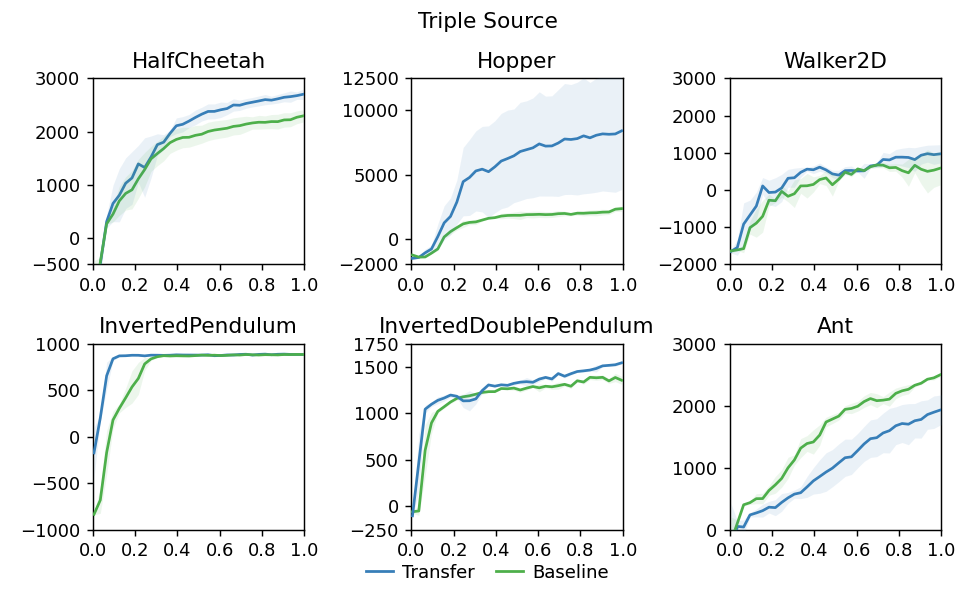
\includegraphics[width=0.7\textwidth]{figures/triple}
			\caption{Results from Sasso, Remo, Matthia Sabatelli, and Marco A. Wiering. "Fractional transfer learning for deep model-based reinforcement learning." arXiv preprint arXiv:2108.06526 (2021)}
		\end{figure}
	

\end{frame}

\end{document}
